\documentclass[semifinal]{cpecmu}

%% This is a sample document demonstrating how to use the CPECMU
%% project template. If you are having trouble, see "cpecmu.pdf" for
%% documentation.

\projectNo{P004-2}
\acadyear{2025}

\titleTH{การจัดการซัพพลายเชนด้วยบล็อกเชน และ ไอโอที }
\titleEN{Blockchain and IoTs in Supply Chain Management }

\author{นางสาวนันท์นภัส ศิริธนาโชคไพศาล }{Nunnapat Sirithanachokpaisan}{650610776}
\author{นางสาวปิ่นนารี พร้อมมิตร }{Pinnaree Prommitr}{650610785}
\author{นายผืนป่า จำปาศรี }{Phuenpa Champasri}{650612090}

\cpeadvisor{anya}
\cpecommittee{trasapong}
\cpecommittee{navadon}


%% Some possible packages to include:
\usepackage[final]{graphicx} % for including graphics

%% Add bookmarks and hyperlinks in the document.
\PassOptionsToPackage{hyphens}{url}
\usepackage[colorlinks=true,allcolors=Blue4,citecolor=red,linktoc=all]{hyperref}
\def\UrlLeft#1\UrlRight{$#1$}

%% Needed just by this example, but maybe not by most reports
\usepackage{afterpage} % for outputting
\usepackage{pdflscape} % for landscape figures and tables. 
\usepackage{float}
\usepackage{hyperref}
%% Some other useful packages. Look these up to find out how to use
%% them.
% \usepackage{natbib}    % for author-year citation styles
% \usepackage{txfonts}
% \usepackage{appendix}  % for appendices on a per-chapter basis
% \usepackage{xtab}      % for tables that go over multiple pages
% \usepackage{subfigure} % for subfigures within a figure
% \usepackage{pstricks,pdftricks} % for access to special PostScript and PDF commands
% \usepackage{nomencl}   % if you have a list of abbreviations

%% if you're having problems with overfull boxes, you may need to increase
%% the tolerance to 9999
% \tolerance=9999

\bibliographystyle{plain}
% \bibliographystyle{IEEEbib}

% \renewcommand{\topfraction}{0.85}
% \renewcommand{\textfraction}{0.1}
% \renewcommand{\floatpagefraction}{0.75}

%% Example for glossary entry
%% Need to use glossary option
%% See glossaries package for complete documentation.
\ifglossary
  \newglossaryentry{lorem ipsum}{
    name=lorem ipsum,
    description={derived from Latin dolorem ipsum, translated as ``pain itself''}
  }
\fi

%% Uncomment this command to preview only specified LaTeX file(s)
%% imported with \include command below.
%% Any other file imported via \include but not specified here will not
%% be previewed.
%% Useful if your report is large, as you might not want to build
%% the entire file when editing a certain part of your report.
% \includeonly{chapters/intro,chapters/background}

\begin{document}
\maketitle
\makesignature

\ifproject
\begin{abstractTH}

โครงงานนี้มีวัตถุประสงค์เพื่อพัฒนาแพลตฟอร์มที่ใช้เทคโนโลยีบล็อกเชน และ อินเทอร์เน็ตทุกสรรพสิ่ง หรือ ไอโอที ในการจัดการซัพพลายเชนของอาหารแช่แข็ง โดยเน้นการติดตามและบันทึกข้อมูลอุณหภูมิแบบเรียลไทม์ ระบบที่พัฒนาขึ้นสามารถแจ้งเตือนอัตโนมัติเมื่ออุณหภูมิของสินค้าอยู่นอกช่วงที่กำหนด และช่วยให้สามารถตรวจสอบย้อนหลังข้อมูลได้อย่างโปร่งใสและปลอดภัย เพื่อลดการสูญเสียของอาหารแช่แข็ง
ที่เกิดจากอุณหภูมิที่ไม่เหมาะสมระหว่างการขนส่ง
ระบบประกอบด้วยส่วนสำคัญ ได้แก่ การบันทึกข้อมูลสินค้าโดยเจ้าหน้าที่ การใช้เซ็นเซอร์ IoTs สำหรับวัดอุณหภูมิและส่งข้อมูลไปยังระบบกลางแบบเข้ารหัส การใช้ระบบการติดตามแบบเรียลไทม์บน บล็อกเชน เพื่อยืนยันและบันทึกข้อมูลโดยอัตโนมัติ และการพัฒนาอินเทอร์เฟซสำหรับเจ้าหน้าที่ในการตรวจสอบข้อมูล วิเคราะห์สถานะสินค้า และรับการแจ้งเตือนเมื่อมีค่าผิดปกติ
โครงงานนี้ยังมุ่งเน้นการศึกษาและทดสอบประสิทธิภาพของบล็อกเชน และ อินเทอร์เน็ตทุกสรรพสิ่ง หรือ ไอโอทีในการปรับปรุงกระบวนการจัดการซัพพลายเชนของอาหาร
แช่แข็ง โดยคาดหวังว่านวัตกรรมนี้จะช่วยเพิ่ม
ความโปร่งใส ลดความสูญเสีย และเสริมสร้างความเชื่อมั่นในคุณภาพของสินค้าอาหารแช่แข็งในห่วงโซ่อุปทาน                                                             
\end{abstractTH}

\begin{abstract}

This project aims to develop a platform utilizing Blockchain technology and the Internet of Things (IoTs) for managing the supply chain of frozen food, with a focus on real-time temperature tracking and recording. The developed system can automatically send alerts when the product's temperature falls outside the predefined range and enables transparent and secure traceability to reduce frozen food losses caused by improper temperature conditions during transportation.
The system comprises key components, including product data recording by personnel, the use of IoTs sensors to measure temperature and transmit encrypted data to the central system, an intelligent tracking system based on Blockchain for automatic data verification and recording, and an interface for personnel to monitor data, analyze product status, and receive notifications in case of anomalies.
This project also aims to study and test the effectiveness of Blockchain and IoTs in improving the frozen food supply chain management process. It is expected that this innovation will enhance transparency, reduce losses, and strengthen confidence in the quality of frozen food products within the supply chain.
\end{abstract}

\iffalse
\begin{dedication}
This document is dedicated to all Chiang Mai University students.

Dedication page is optional.
\end{dedication}
\fi % \iffalse

\begin{acknowledgments}


โครงงานนี้จะไม่สามารถสำเร็จลุล่วงไปได้ หากไม่ได้รับความอนุเคราะห์และการสนับสนุนจากหลายฝ่าย ข้าพเจ้าขอแสดงความขอบคุณเป็นอย่างยิ่งต่อ รศ.ดร.อัญญา อาภาวัชรุตม์ อาจารย์ที่ปรึกษาโครงงาน ที่สละเวลาอันมีค่าให้คำแนะนำ ให้แนวคิด และชี้แนะแหล่งความรู้ที่จำเป็นสำหรับการพัฒนาระบบฮาร์ดเเวร์และเว็บแอปพลิเคชั่น ตลอดจนช่วยตรวจสอบและแก้ไขข้อบกพร่องต่าง ๆ ด้วยความเอาใจใส่มาโดยตลอด
นอกจากนี้ ข้าพเจ้าขอขอบพระคุณ รศ.ดร. ตรัสพงศ์ ไทยอุปถัมภ์ และ ผศ.ดร. นวดนย์ คุณเลิศกิจ ที่ให้คำปรึกษาและข้อเสนอแนะอันเป็นประโยชน์ จนทำให้โครงงานนี้มีความสมบูรณ์ยิ่งขึ้น
ขอขอบคุณเพื่อนๆ และรุ่นพี่ทุกท่าน ที่คอยให้คำแนะนำ ให้กำลังใจ และเป็นแรงสนับสนุนตลอดมา ซึ่งเป็นพลังผลักดันสำคัญที่ทำให้ข้าพเจ้ามุ่งมั่นและตั้งใจทำงานจนสามารถพัฒนาโครงงานนี้จนสำเร็จ
สุดท้ายนี้ ข้าพเจ้าขอขอบพระคุณทุกท่านที่ไม่ได้เอ่ยนาม ณ ที่นี้ ซึ่งได้ให้ความช่วยเหลือและสนับสนุนโครงงานในรูปแบบต่างๆ ตลอดระยะเวลาการดำเนินงาน ขอบพระคุณเป็นอย่างสูง


\acksign{2026}{3}{1}
\end{acknowledgments}%
\fi % \ifproject

\contentspage

\ifproject
\figurelistpage

\tablelistpage
\fi % \ifproject

% \abbrlist % this page is optional

% \symlist % this page is optional

% \preface % this section is optional


\pagestyle{empty}\cleardoublepage
\normalspacing \setcounter{page}{1} \pagenumbering{arabic} \pagestyle{cpecmu}

\chapter{\ifenglish Introduction\else บทนำ\fi}

\section{\ifenglish Project rationale\else ที่มาของโครงงาน\fi}

\par
ปัจจุบัน ระบบห่วงโซ่อุปทานมีบทบาทสำคัญในการขนส่งสินค้า โดยเฉพาะสินค้าที่ต้องควบคุมอุณหภูมิ เช่น อาหารแช่แข็ง ซึ่งจำเป็นต้องได้รับการดูแลอย่างเข้มงวดตลอดกระบวนการขนส่ง เพื่อป้องกันการเสื่อมสภาพของสินค้า อย่างไรก็ตาม ระบบห่วงโซ่อุปทานแบบดั้งเดิมยังคงเผชิญกับปัญหาหลายประการ เช่น การขาดความโปร่งใสในการตรวจสอบย้อนกลับ การบันทึกข้อมูลที่ไม่มีประสิทธิภาพ และการรายงานความผิดปกติที่ล่าช้า ซึ่งอาจส่งผลให้สินค้าได้รับความเสียหายและก่อให้เกิดความสูญเสียทางเศรษฐกิจ

เทคโนโลยีบล็อกเชน (Blockchain) และอินเทอร์เน็ตของสรรพสิ่ง (Internet of Things: IoT)
สามารถช่วยแก้ไขปัญหาดังกล่าวได้ โดยบล็อกเชนทำหน้าที่เป็นระบบจัดเก็บข้อมูลแบบกระจายศูนย์ 
(Decentralized Ledger) ซึ่งมีความปลอดภัยสูงและสามารถตรวจสอบย้อนกลับข้อมูลได้อย่างโปร่งใส
ข้อมูลเกี่ยวกับอุณหภูมิและสถานะของสินค้าตลอดเส้นทางขนส่งจะถูกบันทึกลงในบล็อกเชน และไม่สามารถ
เปลี่ยนแปลงหรือปลอมแปลงได้โดยไม่ได้รับอนุญาต ขณะเดียวกัน อินเทอร์เน็ตของสรรพสิ่งมีบทบาทสำคัญใน
การเก็บรวบรวมข้อมูลแบบเรียลไทม์ผ่านเซ็นเซอร์ที่ติดตั้งอยู่ในระบบขนส่ง ซึ่งช่วยให้สามารถติดตามและเฝ้าระวังอุณหภูมิของสินค้าได้อย่างต่อเนื่อง หากตรวจพบอุณหภูมิที่ผิดปกติ ระบบสามารถแจ้งเตือนอัตโนมัติไปยังผู้ที่เกี่ยวข้องเพื่อดำเนินการแก้ไขได้ทันที
\par
ด้วยเหตุนี้ โครงการนี้จึงมุ่งเน้นการพัฒนาและประยุกต์ใช้เทคโนโลยีบล็อกเชนและอินเทอร์เน็ตของสรรพสิ่ง
เพื่อบริหารจัดการห่วงโซ่อุปทานของอาหารแช่แข็ง โดยมีเป้าหมายเพื่อเพิ่มความโปร่งใสของข้อมูล ลดความสูญเสียของสินค้า และสร้างมาตรฐานใหม่ในการขนส่งสินค้าที่ต้องควบคุมอุณหภูมิให้มีประสิทธิภาพยิ่งขึ้น


\section{\ifenglish Objectives\else วัตถุประสงค์ของโครงงาน\fi}
\begin{enumerate}
    \item เพื่อพัฒนาแพลตฟอร์มที่ใช้บล็อกเชน (Blockchain) และอินเทอร์เน็ตของสรรพสิ่ง (IoT) ในการติดตามและบันทึกข้อมูลอุณหภูมิของอาหารแช่แข็งแบบเรียลไทม์
    \item เพื่อออกแบบและพัฒนาระบบที่สามารถแจ้งเตือนอัตโนมัติเมื่ออุณหภูมิของสินค้าอยู่นอกช่วงที่กำหนด
    \item \sloppy เพื่อสร้างระบบที่สามารถตรวจสอบย้อนกลับข้อมูลของอาหารแช่แข็งตลอดซัพพลายเชน (Supply Chain) ได้อย่างโปร่งใสและปลอดภัย
    \item เพื่อลดการสูญเสียของอาหารแช่แข็งอันเนื่องมาจากอุณหภูมิที่ไม่เหมาะสมระหว่างการขนส่ง
    \item เพื่อศึกษาและทดสอบประสิทธิภาพของระบบบล็อกเชน (Blockchain) และอินเทอร์เน็ตของสรรพสิ่ง (IoT) ในการปรับปรุงกระบวนการจัดการซัพพลายเชน (Supply Chain) ของอาหารแช่แข็ง
\end{enumerate}

\section{\ifenglish Project scope\else ขอบเขตของโครงงาน\fi}

\subsection{\ifenglish Hardware scope\else ขอบเขตด้านฮาร์ดแวร์\fi}
\sloppy
ในด้านฮาร์ดแวร์ โครงงานนี้จะเน้นการพัฒนาและติดตั้งอุปกรณ์ที่ใช้ในการตรวจจับอุณหภูมิของอาหารแช่แข็ง
ตลอดการขนส่ง โดยจะใช้เซ็นเซอร์อินเทอร์เน็ตของสรรพสิ่ง (IoT) ที่สามารถเก็บข้อมูลอุณหภูมิแบบเรียล
ไทม์และส่งข้อมูลเหล่านี้ไปยังระบบคลาวด์หรือบล็อกเชน (Blockchain) สำหรับการจัดเก็บและตรวจสอบ
ข้อมูล เซ็นเซอร์ที่ใช้จะต้องมีความแม่นยำสูง สามารถทำงานได้ในอุณหภูมิที่ต่ำ และเชื่อมต่อกับเครือข่ายอินเทอร์เน็ตของสรรพสิ่ง (IoT) ได้อย่างมีประสิทธิภาพ ซึ่งระบบเครือข่ายจะรองรับการส่งข้อมูลจาก
เซ็นเซอร์ไปยังเซิร์ฟเวอร์หลักเพื่อการประมวลผลและการบันทึกลงในบล็อกเชน (Blockchain)

\subsection{\ifenglish Software scope\else ขอบเขตด้านซอฟต์แวร์\fi}
\sloppy
ในด้านซอฟต์แวร์ โครงงานนี้จะพัฒนาระบบที่สามารถบันทึกข้อมูลการขนส่งและอุณหภูมิของสินค้าแบบเรียลไทม์โดยใช้ Blockchain ซึ่งจะทำหน้าที่เป็นระบบฐานข้อมูลที่มีความปลอดภัยสูงและไม่สามารถปลอมแปลงข้อมูลได้ ระบบจะสามารถบันทึกการเปลี่ยนแปลงของอุณหภูมิที่เกิดขึ้นระหว่างการขนส่ง โดยข้อมูลทุกชนิดจะถูกจัดเก็บใน Blockchain พร้อมกับข้อมูลเกี่ยวกับตำแหน่งของสินค้าและสถานะการขนส่ง การใช้ Blockchain ยังจะช่วยให้สามารถตรวจสอบย้อนกลับข้อมูลการขนส่งและการดูแลสินค้าผ่านระบบแบบกระจายศูนย์ได้อย่างโปร่งใสและปลอดภัย สำหรับระบบการแจ้งเตือนอัตโนมัติ จะถูกพัฒนาขึ้นเพื่อส่งข้อความแจ้งเตือนเมื่ออุณหภูมิของสินค้าอยู่นอกช่วงที่กำหนดไว้ ระบบจะแจ้งเตือนผู้ที่เกี่ยวข้องเพื่อให้ดำเนินการแก้ไขได้ทันที หากตรวจพบการผิดปกติในการขนส่ง นอกจากนี้ยังจะมีการพัฒนาแอปพลิเคชันสำหรับผู้ใช้งานที่สามารถติดตามสถานะของการขนส่งและการบันทึกข้อมูลอุณหภูมิได้จากทุกที่ผ่านอุปกรณ์ที่เชื่อมต่ออินเทอร์เน็ต

\section{\ifenglish Expected outcomes\else ประโยชน์ที่ได้รับ\fi}
\sloppy
\begin{enumerate}
    \item ช่วยให้สามารถติดตามอุณหภูมิของอาหารแช่แข็งในระหว่างการขนส่งแบบเรียลไทม์ และสามารถแจ้งเตือนเมื่ออุณหภูมิของสินค้าผิดปกติ ทำให้สามารถดำเนินการแก้ไขได้ทันที ซึ่งจะช่วยป้องกันการเสื่อมสภาพของสินค้าและลดการสูญเสียทางเศรษฐกิจจากการขนส่งที่ไม่เหมาะสม
    \item การใช้บล็อกเชน (Blockchain) ช่วยให้ข้อมูลเกี่ยวกับอุณหภูมิและสถานะของสินค้าในระหว่างการขนส่งถูกบันทึกอย่างโปร่งใสและไม่สามารถปลอมแปลงได้ ซึ่งทำให้ผู้ที่เกี่ยวข้องสามารถตรวจสอบย้อนกลับข้อมูลได้อย่างปลอดภัยและเชื่อถือได้
    \item ระบบสามารถแจ้งเตือนอัตโนมัติเมื่ออุณหภูมิของสินค้าอยู่นอกช่วงที่กำหนด ทำให้สามารถดำเนินการแก้ไขได้ทันที ลดความเสี่ยงในการสูญเสียสินค้าและเพิ่มประสิทธิภาพในการขนส่ง
    \item การใช้เทคโนโลยีบล็อกเชน (Blockchain) และอินเทอร์เน็ตของสรรพสิ่ง (IoT) ช่วยในการจัดเก็บและติดตามข้อมูลแบบอัตโนมัติ ลดต้นทุนในการขนส่งและการจัดการซัพพลายเชนได้อย่างมีประสิทธิภาพ และสามารถปรับปรุงกระบวนการทำงานในองค์กรได้
    \item สร้างมาตรฐานใหม่ในการขนส่งอาหารแช่แข็ง โดยมีการใช้เทคโนโลยีขั้นสูงในการติดตามและควบคุมอุณหภูมิของสินค้า ช่วยยกระดับคุณภาพการขนส่งในอุตสาหกรรมนี้ให้มีความน่าเชื่อถือและมีประสิทธิภาพมากยิ่งขึ้น
\end{enumerate}

\section{\ifenglish Technology and tools\else เทคโนโลยีและเครื่องมือที่ใช้\fi}

\subsection{\ifenglish Hardware technology\else เทคโนโลยีด้านฮาร์ดแวร์\fi}
\subsubsection{บอร์ดคิดไบร์ท (KidBright Board)}
\textbf{เหตุผลที่เลือกใช้:}
\begin{itemize}
    \item เป็นเครื่องมือสำหรับการเรียนรู้ด้านอินเทอร์เน็ตของสรรพสิ่ง (Internet of Things: IoT) โดยเฉพาะ ทำให้เหมาะสมสำหรับการศึกษาพื้นฐานการเขียนโปรแกรมและพัฒนาอุปกรณ์ IoT ที่สามารถนำไปประยุกต์ใช้ในโครงการได้
    \item มีความสะดวกต่อการใช้งานและเหมาะสำหรับโครงการขนาดเล็ก โดยสามารถเริ่มต้นใช้งานได้อย่างรวดเร็ว จึงเหมาะสำหรับการพัฒนาเซ็นเซอร์เพื่อตรวจสอบอุณหภูมิในโครงการนี้
    \item มีต้นทุนต่ำ ทำให้เหมาะสมสำหรับการทดลองและพัฒนาในระดับต้นหรือการสร้างต้นแบบ (Prototype)
    \item รองรับการเชื่อมต่อกับอุปกรณ์ IoT และเซ็นเซอร์ต่าง ๆ ซึ่งช่วยให้สามารถเก็บข้อมูลอุณหภูมิได้แบบเรียลไทม์
\end{itemize}


\subsubsection{เซ็นเซอร์วัดอุณหภูมิแบบดิจิทัล ดีเอส 18 บี 20 (DS18B20 Sensor)}
\textbf{เหตุผลที่เลือกใช้:}
\begin{itemize}
    \item รองรับการวัดอุณหภูมิในช่วงกว้าง ตั้งแต่ -55\textdegree C ถึง +125\textdegree C ซึ่งสามารถครอบคลุมช่วงอุณหภูมิที่ใช้ในกระบวนการขนส่งอาหารแช่แข็งได้เป็นอย่างดี
    \item มีความแม่นยำสูง โดยมีค่าความคลาดเคลื่อนเพียง $\pm$ 0.5\textdegree C ในช่วงอุณหภูมิระหว่าง -10\textdegree C ถึง +85\textdegree C ซึ่งเหมาะสมสำหรับการควบคุมอุณหภูมิของอาหารแช่แข็งที่ต้องรักษาอุณหภูมิให้อยู่ในช่วงที่กำหนด
    \item รองรับการเชื่อมต่อแบบวัน-ไวร์ (1-Wire) โดยใช้สายสัญญาณเพียงเส้นเดียวสำหรับการรับส่งข้อมูล ซึ่งช่วยลดความซับซ้อนของการเดินสายไฟและการติดตั้ง
\end{itemize}


\subsection{\ifenglish Software technology\else เทคโนโลยีด้านซอฟต์แวร์\fi}
\subsubsection{รีแอกต์ (React)}
\textbf{เหตุผลที่เลือกใช้:}
\begin{itemize}
    \item มีประสิทธิภาพสูงและรองรับการพัฒนา ส่วนต่อประสานกับผู้ใช้ (UI) แบบไดนามิกที่ตอบสนองรวดเร็ว (Responsive UI)
    \item รองรับการใช้งานร่วมกับ ไทป์สคริปต์ (TypeScript) ซึ่งช่วยให้การพัฒนามีความปลอดภัยจากข้อผิดพลาดด้านประเภทข้อมูล
\end{itemize}

\subsubsection{จาวาสคริปต์ (JavaScript)}
\textbf{เหตุผลที่เลือกใช้:}
\begin{itemize}
    \item เป็นภาษาหลักในการพัฒนาเว็บแอปพลิเคชันที่สามารถทำงานได้ทั้งในส่วนหน้า (Frontend) และส่วนหลัง (Backend)
    \item มีไลบรารีและเฟรมเวิร์กที่รองรับการทำงานร่วมกับ บล็อกเชน (Blockchain) และ ไอโอที (IoT)
    \item รองรับการทำงานแบบ แอสิงโครนัส (Asynchronous) ซึ่งช่วยให้การประมวลผลข้อมูลจากเซ็นเซอร์ไอโอที (IoT Sensor) มีประสิทธิภาพมากขึ้น
\end{itemize}
\subsubsection{ไทป์สคริปต์ (TypeScript)}
\textbf{เหตุผลที่เลือกใช้:}
\begin{itemize}
    \item เพิ่มความปลอดภัยให้กับโค้ดด้วยการกำหนดประเภทของตัวแปร ลดข้อผิดพลาดในระหว่างการพัฒนา
    \item ช่วยให้การพัฒนาโค้ดมีโครงสร้างที่ดีขึ้น และง่ายต่อการบำรุงรักษา
    \item รองรับการทำงานร่วมกับ รีแอกต์ (React) และ โนด.เจเอส (Node.js) ได้เป็นอย่างดี
\end{itemize}

\subsubsection{โนด.เจเอส (Node.js)}
\textbf{เหตุผลที่เลือกใช้:}
\begin{itemize}
    \item สามารถประมวลผลแบบ แอสิงโครนัส (Asynchronous) ได้ ทำให้เหมาะกับระบบที่ต้องรับส่งข้อมูลแบบเรียลไทม์จากเซ็นเซอร์ไอโอที (IoT Sensor)
    \item รองรับการทำงานร่วมกับ เอ็กซ์เพรส.เจเอส (Express.js) ในการพัฒนา เอพีไอ (API) สำหรับเชื่อมต่อกับ บล็อกเชน (Blockchain) และฐานข้อมูล
\end{itemize}
\subsubsection{เอ็กซ์เพรส.เจเอส (Express.js)}
\textbf{เหตุผลที่เลือกใช้:}
\begin{itemize}
    \item เป็นเฟรมเวิร์กสำหรับพัฒนาเว็บที่มีขนาดเล็กและมีประสิทธิภาพสูงในการสร้าง เอพีไอแบบเรสต์ฟูล (RESTful API)
    \item ช่วยให้สามารถจัดการเส้นทาง (Routing) และ มิดเดิลแวร์ (Middleware) ได้อย่างง่ายดาย
    \item รองรับการทำงานร่วมกับ โนด.เจเอส (Node.js) และสามารถเชื่อมต่อกับ บล็อกเชน (Blockchain) และ ไอโอที (IoT) ได้ง่าย
\end{itemize}

\subsubsection{อินซอมเนีย (Insomnia)}
\sloppy
\textbf{เหตุผลที่เลือกใช้:}
\begin{itemize}
    \item ใช้สำหรับทดสอบ เอพีไอแบบเรสต์ (REST API) เพื่อให้แน่ใจว่าระบบสามารถรับ-ส่งข้อมูลได้อย่างถูกต้อง
    \item รองรับการทำงานกับ การพิสูจน์ตัวตนของเอพีไอ (API Authentication) ทำให้สามารถทดสอบการเชื่อมต่อกับ บล็อกเชน (Blockchain) ได้ง่ายขึ้น
    \item มีส่วนต่อประสานกับผู้ใช้ (UI) ที่ใช้งานง่ายและช่วยให้การดีบั๊ก เอพีไอ (API) มีประสิทธิภาพมากขึ้น
\end{itemize}

\subsubsection{ไฮเปอร์เลดเจอร์ แฟบริก (Hyperledger Fabric)}
\sloppy
\textbf{เหตุผลที่เลือกใช้:}
\begin{itemize}
    \item เป็นแพลตฟอร์ม บล็อกเชน (Blockchain) ระดับองค์กรที่มีความปลอดภัยและรองรับการกำหนดสิทธิ์การเข้าถึงข้อมูล
    \item รองรับการทำ สมาร์ทคอนแทร็กต์ (Smart Contract) ซึ่งช่วยให้สามารถควบคุมและตรวจสอบข้อมูลอุณหภูมิของสินค้าได้อย่างปลอดภัย
    \item สามารถเชื่อมต่อกับ เซ็นเซอร์ไอโอที (IoT Sensor) และบันทึกข้อมูลแบบไม่สามารถเปลี่ยนแปลงได้ ทำให้ระบบมีความโปร่งใสและตรวจสอบได้ง่าย
\end{itemize}

\section{\ifenglish Project plan\else แผนการดำเนินงาน\fi}
\begin{table}[H]
    \centering
    \label{tab:project-timeline} 
    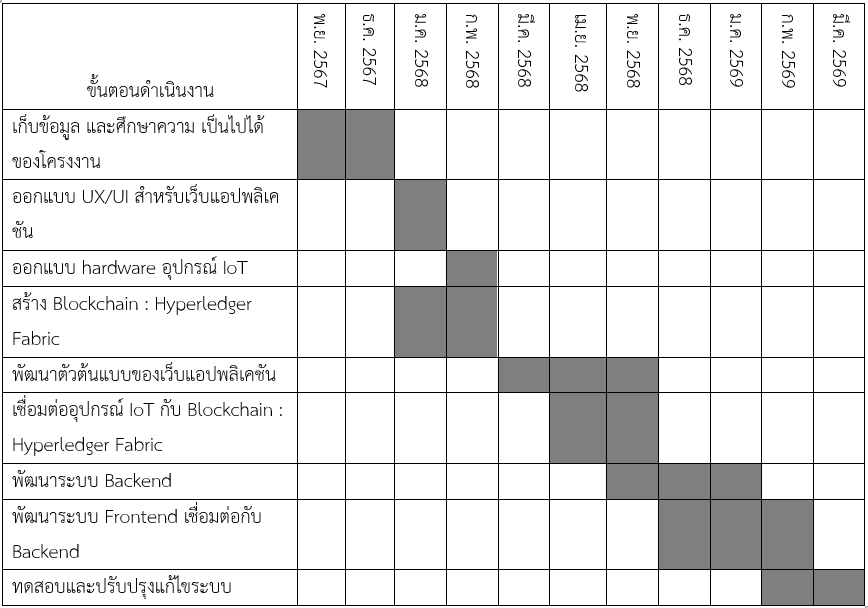
\includegraphics[width=\textwidth]{workplan.png}
    \caption{แผนการดำเนินงานโครงการ} 
\end{table}


\section{\ifenglish Roles and responsibilities\else บทบาทและความรับผิดชอบ\fi}
\begin{enumerate}
    \item นางสาวนันท์นภัส ศิริธนาโชคไพศาล: พัฒนาโครงสร้างส่วนหน้า (Frontend) สำหรับการใช้งานฟังก์ชันต่าง ๆ
    \begin{itemize}
        \item ออกแบบและพัฒนาส่วนติดต่อผู้ใช้ (User Interface) ให้ใช้งานได้สะดวกและเหมาะสม
        \item พัฒนาหน้าล็อกอินที่มีระบบตรวจสอบสิทธิ์ผู้ใช้ เพื่อให้สามารถเข้าถึงข้อมูลได้อย่างปลอดภัย
        \item สร้างระบบสำหรับการเข้าถึงและแสดงผลฟังก์ชันต่าง ๆ ภายในแอปพลิเคชัน เช่น การแสดงผลอุณหภูมิแบบเรียลไทม์ของสินค้าระหว่างการขนส่ง และการเพิ่มข้อมูลการจัดส่งสินค้า เพื่อให้สามารถติดตามสถานะของสินค้าได้อย่างแม่นยำ
        \item เชื่อมต่อโครงสร้างส่วนหน้า (Frontend) กับโครงสร้างส่วนหลัง (Backend) เพื่อให้ข้อมูลสามารถอัปเดตและแสดงผลแบบเรียลไทม์ รวมถึงพัฒนาอินเทอร์เฟซที่รองรับการแจ้งเตือนเมื่อเกิดความผิดปกติ
    \end{itemize}
    
    \item นายผืนป่า จำปาศรี: พัฒนาอุปกรณ์ตรวจจับอุณหภูมิ (Hardware)
    \begin{itemize}
        \item ออกแบบและพัฒนาอุปกรณ์เซ็นเซอร์ตรวจจับอุณหภูมิที่สามารถติดตั้งภายในระบบขนส่งสินค้า
        \item พัฒนาแบบจำลองการวิเคราะห์ข้อมูลอุณหภูมิ เพื่อประเมินความเสถียรของสภาพแวดล้อมระหว่างการขนส่ง และตรวจจับความผิดปกติที่อาจส่งผลต่อคุณภาพของอาหารแช่แข็ง
        \item ปรับปรุงอุปกรณ์ให้สามารถทำงานได้อย่างมีประสิทธิภาพภายใต้สภาพแวดล้อมที่
        หลากหลาย รวมถึงพัฒนาโหมดการทำงานที่ช่วยลดการใช้พลังงานในระหว่างการขนส่ง
        \item เชื่อมต่อเซ็นเซอร์เข้ากับระบบอินเทอร์เน็ตของสรรพสิ่ง (IoT) เพื่อให้ข้อมูลอุณหภูมิถูกบันทึกและส่งไปยังบล็อกเชน (Blockchain) ได้แบบเรียลไทม์
    \end{itemize}

    
    \item นางสาวปิ่นนารี พร้อมมิตร: พัฒนาโครงสร้างส่วนหลัง (Backend) การจัดสร้างบล็อกเชน (Blockchain) และการบริหารจัดการฐานข้อมูล
    \begin{itemize}
        \item ออกแบบและพัฒนาฐานข้อมูลกลาง เพื่อใช้ในการจัดเก็บข้อมูลอุณหภูมิ ข้อมูลการขนส่ง และผลการวิเคราะห์คุณภาพของสินค้า
        \item พัฒนาระบบโครงสร้างส่วนหลัง (Backend) ที่รองรับการประมวลผลข้อมูลแบบเรียลไทม์ และสามารถเชื่อมต่อกับอุปกรณ์อินเทอร์เน็ตของสรรพสิ่ง (IoT) เพื่อรับข้อมูลอุณหภูมิจากเซ็นเซอร์ที่ติดตั้งภายในระบบขนส่ง
        \item สร้างระบบบล็อกเชน (Blockchain) เพื่อใช้เป็นแพลตฟอร์มสำหรับการจัดเก็บข้อมูลอุณหภูมิและสถานะของสินค้าตลอดเส้นทางขนส่ง ซึ่งช่วยให้ข้อมูลมีความปลอดภัย ไม่สามารถเปลี่ยนแปลงหรือปลอมแปลงได้โดยไม่ได้รับอนุญาต
        \item พัฒนาระบบแจ้งเตือนอัตโนมัติ เมื่อมีการเปลี่ยนแปลงของอุณหภูมิที่อาจส่งผลกระทบต่อคุณภาพสินค้า โดยแจ้งเตือนไปยังผู้ที่เกี่ยวข้องเพื่อให้สามารถดำเนินการแก้ไขได้อย่างทันท่วงที
        \item 
    \end{itemize}
    
\end{enumerate}

\section{\ifenglish%
Impacts of this project on society, health, safety, legal, and cultural issues
\else%
ผลกระทบด้านสังคม สุขภาพ ความปลอดภัย กฎหมาย และวัฒนธรรม
\fi}

\subsection{ด้านสังคม}
โครงการนี้จะมีผลกระทบทางสังคมโดยการเพิ่มความโปร่งใสและการตรวจสอบย้อนกลับในกระบวนการขนส่งสินค้าที่ต้องควบคุมอุณหภูมิ เช่น อาหารแช่แข็ง ซึ่งส่งผลให้ผู้บริโภคได้รับสินค้าที่มีคุณภาพและปลอดภัยมากขึ้น การใช้เทคโนโลยีบล็อกเชน (Blockchain) ช่วยลดปัญหาการปลอมแปลงข้อมูล และเพิ่มความมั่นใจในระบบห่วงโซ่อุปทาน ซึ่งสามารถช่วยส่งเสริมการพัฒนาเศรษฐกิจในท้องถิ่นและยกระดับมาตรฐานของธุรกิจในภาคการขนส่งสินค้า

\subsection{ด้านสุขภาพ}
การควบคุมอุณหภูมิในการขนส่งอาหารแช่แข็งมีผลโดยตรงต่อสุขภาพของผู้บริโภค การใช้ระบบอินเทอร์เน็ตของสรรพสิ่ง (Internet of Things: IoT) เพื่อเฝ้าระวังอุณหภูมิอย่างต่อเนื่องจะช่วยลดโอกาสในการเกิดการปนเปื้อนหรือการเสื่อมสภาพของอาหาร ซึ่งสามารถป้องกันโรคที่เกิดจากอาหารที่ไม่ปลอดภัย รวมถึงลดความเสี่ยงจากการแพร่กระจายของโรคระบาดที่เกี่ยวข้องกับการรับประทานอาหาร

\subsection{ด้านความปลอดภัย}
โครงการนี้สามารถเพิ่มความปลอดภัยในการขนส่งอาหารแช่แข็งได้ ด้วยการติดตามสถานะของอุณหภูมิและสถานที่ขนส่งแบบเรียลไทม์ ผ่านเซ็นเซอร์ IoT และการตรวจสอบข้อมูลบนบล็อกเชน เมื่อมีการแจ้งเตือนความผิดปกติในอุณหภูมิหรือเส้นทางการขนส่ง จะสามารถดำเนินการแก้ไขได้ทันที เพื่อป้องกันความเสียหายของสินค้าและอันตรายที่อาจเกิดขึ้น

\subsection{ด้านกฎหมาย}
เทคโนโลยีบล็อกเชน (Blockchain) ช่วยให้สามารถบันทึกข้อมูลอย่างโปร่งใสและไม่สามารถแก้ไขได้โดยไม่ได้รับอนุญาต ซึ่งช่วยให้สามารถตรวจสอบการปฏิบัติตามกฎหมายและระเบียบข้อบังคับได้ง่ายขึ้น โดยเฉพาะในด้านการควบคุมการขนส่งสินค้าที่ต้องควบคุมอุณหภูมิ เช่น อาหารแช่แข็ง การบังคับใช้กฎหมายที่เกี่ยวข้องกับการขนส่งอาหารและสุขอนามัยจะมีประสิทธิภาพมากขึ้นเมื่อมีระบบการตรวจสอบที่ชัดเจน

\subsection{ด้านวัฒนธรรม}
การใช้เทคโนโลยีใหม่ๆ ในการขนส่งและควบคุมอุณหภูมิอาจมีผลต่อการเปลี่ยนแปลงวิธีการทำงานของภาคการขนส่ง โดยเฉพาะอย่างยิ่งในวัฒนธรรมองค์กรที่มุ่งเน้นการปรับปรุงและพัฒนาเทคโนโลยีใหม่ๆ การนำเทคโนโลยีเหล่านี้มาใช้สามารถกระตุ้นให้เกิดการยอมรับในนวัตกรรมใหม่ในสังคมไทย และเพิ่มขีดความสามารถในการแข่งขันในระดับสากล

\subsection{แนวทางและโยชน์ในการประยุกต์ใช้งานโครงงานกับงานในด้านอื่นๆ รวมถึงผลกระทบในด้านสังคมและสิ่งแวดล้อมจากการใช้ความรู้ทางวิศวกรรมที่ได้}
โครงงานนี้สามารถประยุกต์ใช้ในหลายด้าน เช่น
\begin{itemize}
    \item การขนส่งยา – การใช้ระบบบล็อกเชน (Blockchain) และ IoT เพื่อควบคุมอุณหภูมิและสถานะของยาในระหว่างการขนส่ง ทำให้มั่นใจได้ว่ายาที่มีความสำคัญจะไม่สูญเสียคุณภาพและไม่เสี่ยงต่อการถูกปลอมแปลง
    \item การขนส่งผลิตภัณฑ์ทางการแพทย์ – ผลิตภัณฑ์ทางการแพทย์ที่ต้องการการควบคุมอุณหภูมิ เช่น วัคซีนและอุปกรณ์ทางการแพทย์ สามารถได้รับประโยชน์จากระบบนี้
    \item การขนส่งสินค้าอุปโภคบริโภคอื่นๆ – ระบบนี้สามารถขยายไปใช้กับสินค้าประเภทอื่นๆ ที่ต้องการการควบคุมอุณหภูมิหรือสภาพแวดล้อมในการขนส่ง
\end{itemize}

ผลกระทบในด้านสังคมและสิ่งแวดล้อมจากการใช้ความรู้ทางวิศวกรรมที่ได้
จากการใช้เทคโนโลยี IoT และบล็อกเชน (Blockchain) ในการจัดการห่วงโซ่อุปทาน อาจช่วยลดการใช้พลังงานในการขนส่งและลดการปล่อยมลพิษจากการขนส่งที่ไม่เหมาะสม โดยการติดตามเส้นทางการขนส่งและสถานะของสินค้า ทำให้สามารถประหยัดทรัพยากรได้ นอกจากนี้ยังช่วยลดการสูญเสียสินค้าจากการขนส่งที่ผิดพลาด หรือไม่เป็นไปตามมาตรฐาน ซึ่งส่งผลดีต่อสิ่งแวดล้อมโดยการลดขยะและการสูญเสียทรัพยากร

\chapter{\ifenglish Background Knowledge and Theory\else ทฤษฎีที่เกี่ยวข้อง\fi}


การทำโครงงาน เริ่มต้นด้วยการศึกษาค้นคว้า ทฤษฎีที่เกี่ยวข้อง หรือ งานวิจัย/โครงงาน ที่เคยมีผู้นำเสนอไว้แล้ว ซึ่งเนื้อหาในบทนี้ก็จะเกี่ยวกับการอธิบายถึงสิ่งที่เกี่ยวข้องกับโครงงาน เพื่อให้ผู้อ่านเข้าใจเนื้อหาในบทถัดๆ ไปได้ง่ายขึ้น


\section{ทฤษฎีที่เป็นความรู้ในการขนส่งแบบติดตามอุณหภูมิ }

\begin{enumerate}
    \item ระบบทำความเย็น (Cooling System): การลดและรักษาระดับอุณหภูมิหรือการทำความเย็น เพื่อ	ให้สภาพแวดล้อมหรือพื้นที่จัดเก็บมีความเหมาะสมในการเก็บรักษาและขนส่งสินค้า โดยให้ความ		สำคัญกับอุณหภูมิ, ความชื้น และความเข้าใจในสินค้า เพื่อเลือกใช้วิธีการทำความเย็นที่เหมาะสม 	เช่น การใช้น้ำแข็ง, น้ำเย็น, การแช่แข็ง หรือการใช้ระบบสูญญากาศ 
    \item คลังสินค้าห้องเย็น (Cold Storage): พื้นที่จัดเก็บสินค้าที่มีการควบคุมอุณหภูมิภายในให้เหมาะสม 	สำหรับการจัดเก็บสินค้าในช่วงระยะเวลาหนึ่งก่อนการกระจายหรือขนส่งสินค้า เพื่อรักษาคุณภาพ	สินค้าในสภาพแวดล้อมที่มีอุณหภูมิและความชื้นคงที่ โดยทั่วไปอุุณหภูมิภายในคลังสินค้าห้องเย็นจะ	ต่ำกว่า 25 องศาเซลเซียส หรืออาจติดลบ ขึ้นอยู่กับประเภทของสินค้าที่จัดเก็บ
    \item การขนส่งแบบควบคุมอุณหภูมิ (Cold Transpot): การใช้ยานพาหนะที่ออกแบบมาเฉพาะสำหรับ	การขนส่งที่ต้องการติดตาม หรือควบคุมอุณหภูมิ เช่น รถบรรทุกห้องเย็น ที่มีระบบควบคุมอุณหภูมิ	และความชื้นภายใน เพื่อรักษาคุณภาพ และความสดใหม่ของสินค้าระหว่างการขนส่ง
    \item การจัดการโลจิสติกส์โซ่ความเย็น (Cold Chain Management): การวางแผน และควบคุม		กระบวนการทั้งหมดในห่วงโซ่อุปทาน ตั้งแต่การผลิต, การจัดเก็บ, การขนส่ง จนถึงการจัดจำหน่าย 	เพื่อให้สินค้าที่ต้องการควบคุมอุณหภูมิได้รับการดูแลอย่างเหมาะสม
    \item การติดตามและควบคุมอุณหภูมิระหว่างการขนส่ง: การใช้เทคโนโลยี เช่น IoTs และเซนเซอร์วัด		อุณหภูมิ เพื่อตรวจสอบ และบันทึกอุณหภูมิในบรรจุภัณฑ์ที่จัดเก็บสินค้าตลอดระยะเวลาในการขนส่ง	เพื่อให้มมั่นใจว่าสินค้าได้รับการควบคุมอุณหภูมิตามที่กำหนด
    \item การเลือกบรรณจุภัณฑ์ที่เหมาะสมสำหรับการขนส่งควบคุมอุณหภูมิ: การเลือกบรรจุภัณฑ์ที่ีเหมาะสม	เป็นสิ่งสำคัญในการรักษาคุณภาพของสินค้าในระหว่างการขนส่งควบคุมอุณหภูมิ โดยควรมีคุณสมบัติ	ดังนี้
        \begin{itemize}
            \item ความแข็งแรงและทนทาน : เพื่อป้องกันความเสียหายจากแรงกระแทกหรือการกดทับระหว่างการขนส่ง
            \item การป้องกันการรั่วซึม : เพื่อป้องกันการปนเปื้อนจากน้ำ สารเคมี หรือสิ่งสกปรก
            \item ขนาดที่เหมาะสม : เพื่อให้สินค้าเหมาะกับบรรจุภัณฑ์ ไม่แน่นหรือหลวมเกินไป
            \item วัสดุที่ได้รับมาตรฐาน Food Grade : เพื่อความปลอดภัยของผู้บริโภค
        \end{itemize}
    \item การใช้บรรจุภัณฑ์โซ่ความเย็น (Cold Chain Packaging): บรรจุภัณฑ์โซ่ความเย็นถูกออกแบบมาเพื่อ	รักษาอุณหภูมิของสินค้าที่ไวต่อความร้อนในระหว่างการขนส่ง การเลือกใช้บรรจุภัณฑ์เหล่านี้ช่วยลด	ความเสี่ยงในการเสื่อมสภาพของสินค้าและรักษาคุณภาพของผลิตภัณฑ์ 
\end{enumerate}

\section{Blockchain – Hyperledger Fabric }
Hyperledger Fabric เป็นเฟรมเวิร์กบล็อกเชนแบบโอเพ่นซอร์สที่พัฒนาโดยโครงการ Hyperledger ภายใต้การดูแลของ Linux Foundation ออกแบบมาเพื่อการใช้งานในระดับองค์กร  
โดยมีสถาปัตยกรรมแบบโมดูลาร์ที่ช่วยให้สามารถปรับแต่งและขยายระบบได้ตามความต้องการของธุรกิจ 
โดยมีคุณสมบัติเด่นดังนี้ 

\begin{enumerate}
    \item สถาปัตยกรรมแบบโมดูลาร์: ช่วยให้สามารถปรับแต่งส่วนประกอบต่าง ๆ เช่น ฉันทามติ (consensus) และบริการสมาชิก (membership services) เพื่อให้เหมาะสมกับการใช้งานเฉพาะด้าน
    \item การรองรับธุรกรรมที่เป็นความลับ: ด้วยการใช้ช่องทาง (channels) ทำให้สามารถแบ่งปันข้อมูลเฉพาะกับผู้เข้าร่วมที่เกี่ยวข้องเท่านั้น ซึ่งเหมาะสำหรับธุรกิจที่ต้องการความเป็นส่วนตัวสูง 
\end{enumerate}
จากคุณสมบัติต่าง ๆ ข้างต้น เราจึงได้นำ Hyperledger Fabric มาประยุกต์ใช้กับโครงงานดังนี้ 
\begin{enumerate}
    \item การติดตามสินค้า: บล็อกเชนสามารถบันทึกข้อมูลการขนส่งสินค้า เช่น ปริมาณสินค้า สถานที่ และเวลา ทำให้ทุกฝ่ายที่เกี่ยวข้องสามารถตรวจสอบสถานะสินค้าได้แบบเรียลไทม์ 
    \item การตรวจสอบอุณหภูมิ: สำหรับสินค้าที่ต้องการควบคุมอุณหภูมิ เช่น ยา อาหารทะเล หรือผลิตภัณฑ์จากนม การบันทึกข้อมูลอุณหภูมิในบล็อกเชนช่วยให้มั่นใจว่าสินค้าได้รับการจัดเก็บและขนส่งในสภาพแวดล้อมที่เหมาะสม 
    \item ความโปร่งใสและความน่าเชื่อถือ: การใช้บล็อกเชนช่วยให้ข้อมูลการขนส่งไม่สามารถถูกแก้ไขได้ ทำให้ผู้บริโภคและผู้เกี่ยวข้องมั่นใจในคุณภาพและความปลอดภัยของสินค้า
\end{enumerate}

จากการเลือกใช้ Hyperledger Fabric จึงทำให้เกิดประโยชน์ต่าง ๆ มากมายในโครงงานนี้เช่น การลดความซับซ้อนของกระบวนการด้วยการรวบรวมข้อมูลทั้งหมดไว้ในระบบเดียว ทำให้สามารถลดขั้นตอนการประสานงานระหว่างฝ่ายต่าง ๆ และด้วยคุณสมบัติของ Blockchain ที่ข้อมูลไม่สามารถแก้ไขได้ ทำให้สามารถลดความเสี่ยงจากการทุจริตหรือข้อผิดพลาดได้อีกด้วย 
\begin{itemize}
    \item ข้อดี: Hyperledger Fabric เป็น Permissioned Blockchain ที่รองรับ Private Channels ทำให้สามารถกำหนดสิทธิ์การเข้าถึงข้อมูลเฉพาะกลุ่มที่เกี่ยวข้องได้ ช่วยเพิ่มความปลอดภัยและความเป็นส่วนตัวของข้อมูล
    \item ข้อเสีย: โครงสร้างที่ซับซ้อนและต้องมีการตั้งค่าหลายส่วน เช่น Peer Nodes, Orderers และ Membership Services ทำให้การติดตั้งและดูแลระบบต้องใช้ความเชี่ยวชาญเฉพาะด้าน
\end{itemize}

\section{KidBright Board}
\begin{figure}[H]
    \begin{center}
        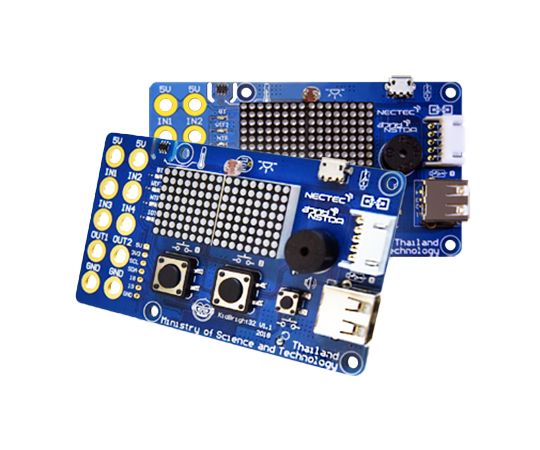
\includegraphics[width=1\textwidth]{chapters/kidbright-transparent.png}
    \end{center}
    \caption[KidBright Board]{KidBright Board}
\end{figure}
KidBright เป็นบอร์ดไมโครคอนโทรลเลอร์ที่พัฒนาโดยคนไทย มีวัตถุประสงค์เพื่อส่งเสริมการเรียนรู้ด้านการเขียนโปรแกรมและอิเล็กทรอนิกส์ในกลุ่มนักเรียนและผู้สนใจ บอร์ดนี้มาพร้อมกับเซ็นเซอร์และอุปกรณ์พื้นฐาน เช่น เซ็นเซอร์วัดแสง (LDR), เซ็นเซอร์วัดอุณหภูมิ, ปุ่มกด, และจอแสดงผล LED 16x8 ทำให้ผู้ใช้สามารถเริ่มต้นพัฒนาโครงการได้ทันที
\begin{itemize}
    \item ข้อดี: KidBright Board เป็นไมโครคอนโทรลเลอร์ที่ออกแบบมาให้ใช้งานง่าย มีฟังก์ชันพื้นฐานในตัว เช่น จอ LED, ปุ่มกด และพอร์ตเชื่อมต่ออุปกรณ์เสริม รองรับการเขียนโปรแกรมแบบบล็อก (Block-based Programming) และภาษา Python ทำให้สามารถพัฒนาโครงงานได้อย่างรวดเร็ว
    \item ข้อเสีย: KidBright Board มีข้อจำกัดด้านประสิทธิภาพเมื่อเทียบกับไมโครคอนโทรลเลอร์ระดับสูง เช่น Raspberry Pi หรือ ESP32 โดยเฉพาะในด้านการประมวลผลข้อมูลจำนวนมากหรือการเชื่อมต่ออินเทอร์เน็ตแบบไร้สาย
\end{itemize}

\section{เซนเซอร์ DS18B20 }
\begin{figure}[H]
    \begin{center}
        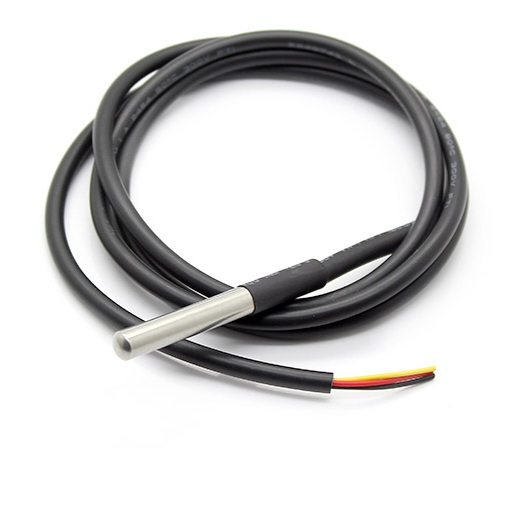
\includegraphics[width=1\textwidth]{chapters/k6xejr.jpg}
    \end{center}
    \caption[เซนเซอร์ DS18B20 ]{เซนเซอร์ DS18B20 }
\end{figure}
DS18B20 เป็นเซ็นเซอร์วัดอุณหภูมิแบบดิจิตอลที่ได้รับความนิยม เนื่องจากความแม่นยำและความสะดวกในการใช้งาน เซ็นเซอร์นี้สามารถวัดอุณหภูมิในช่วง -55°C ถึง +125°C และมีความละเอียดที่ปรับได้ตั้งแต่ 9 ถึง 12 บิต นอกจากนี้ DS18B20 ยังรองรับการเชื่อมต่อแบบ 1-Wire ซึ่งช่วยลดจำนวนสายที่ต้องใช้ในการเชื่อมต่อ
\begin{itemize}
    \item ข้อดี: DS18B20 เป็นเซ็นเซอร์วัดอุณหภูมิแบบดิจิทัลที่มีความแม่นยำสูง รองรับช่วงอุณหภูมิกว้างตั้งแต่ -55°C ถึง +125°C และสามารถสื่อสารผ่านโปรโตคอล 1-Wire ซึ่งช่วยลดจำนวนสายสัญญาณที่ใช้ในการเชื่อมต่อ
    \item ข้อเสีย: เซ็นเซอร์ DS18B20 มีอัตราการตอบสนองที่ช้ากว่าเซ็นเซอร์ประเภทอื่น เช่น เทอร์มิสเตอร์ หรือ RTD ทำให้ไม่เหมาะกับการวัดอุณหภูมิที่ต้องการการเปลี่ยนแปลงแบบเรียลไทม์
\end{itemize}

\section{\ifenglish%
\ifcpe CPE \else ISNE \fi knowledge used, applied, or integrated in this project
\else%
ความรู้ตามหลักสูตรซึ่งถูกนำมาใช้หรือบูรณาการในโครงงาน
\fi
}

ในการพัฒนาโครงงานนี้ได้นำองค์ความรู้จากรายวิชาต่าง ๆ มาประยุกต์ใช้ให้สามารถออกแบบและพัฒนาระบบได้อย่างมีประสิทธิภาพ โดยรายวิชาที่เกี่ยวข้องมีดังนี้
\begin{itemize}
    \item 261207 ฺBasic Computer Engineering Laboratory: นำความรู้เกี่ยวกับการพัฒนาเว็บไซต์โดยใช้ทั้ง JavaScript และ TypeScript รวมถึงการดึงข้อมูลจาก API และหลักการของ HTTP method มาประยุกต์ใช้ในการพัฒนา Front-End และ Back-End ของโครงงานนี้
    \item 261343 Database System Laboratory: นำความรู้เกี่ยวกับการจัดการฐานข้อมูล รวมถึงการใช้งาน Docker ซึ่งเป็นส่วนสำคัญในการสร้างและจัดการ Blockchain ซึ่งเป็นฐานข้อมูลหลักของโครงงานนี้
    \item 261215 Embedded System Laboratory: นำความรู้ในรายวิชานี้มาใช้เพื่อออกแบบชิ้นงานของโครงงาน รวมไปถึงการประดิษฐ์ชิ้นงาน และการเลือกใช้งานบอร์ดหรือเซนเซอร์
    \item 261430 Wireless Network: นำความรู้เกี่ยวกับ Kidbright board ที่ได้เรียนในใช้เรียนเป็นเหตุผลหลักในการเลือกใช้บอร์ดนี้ในโครงงาน
    \item 261200 Object-Oriented Programming: นำแนวคิดเชิงวัตถุมาใช้ในการออกแบบและพัฒนาโครงสร้างต่าง ๆ ในระบบ
    \item 261361 Software Engineering: นำความรู้ในวิชานี้มาวิเคราะห์ความต้องการของผู้ใช้งาน, วางแผนโครงสร้างของระบบ, วางแผนการพัฒนาโครงสร้างของระบบ และ การทดสอบระบบต่าง ๆ ในโครงงานนี้
\end{itemize}
\section{\ifenglish%
Extracurricular knowledge used, applied, or integrated in this project
\else%
ความรู้นอกหลักสูตรซึ่งถูกนำมาใช้หรือบูรณาการในโครงงาน
\fi
}

โครงงานนี้ได้นำความรู้จากแหล่งอื่น ๆ ที่ไม่ได้อยู่ในรายวิชาเรียนหรือหลักสูตรของภาควิชา เพื่อเพิ่มประสิทธิภาพและเสริมสร้างความสามารถของการทำโครงงาน โดยมีรายละเอียดดังนี้
\begin{itemize}
    \item Blockchain – Hyperledger Fabric: โครงงานนี้ได้นำความรู้เกี่ยวกับ Hyperledger Fabric ซึ่งเป็นหนึ่งในเฟรมเวิร์กของ Permissioned Blockchain มาใช้ในการพัฒนาและออกแบบระบบที่เกี่ยวข้องกับการติดตามข้อมูลและการจัดเก็บบันทึกที่มีความปลอดภัยสูง โดยความรู้ที่นำมาใช้ประกอบด้วย
    \begin{enumerate}
        \item โครงสร้างของ Hyperledger Fabric: ระบบที่รองรับการทำงานแบบโมดูลาร์ สามารถกำหนดกลไกการยืนยันตัวตน (Identity Management) และรูปแบบฉันทามติ (Consensus Mechanism) ได้ตามต้องการ
        \item การใช้ Smart Contract (Chaincode): Chaincode ใน Hyperledger Fabric ทำหน้าที่เหมือน Smart Contract ในบล็อกเชนอื่น ๆ โดยใช้ภาษา Go, Node.js หรือ Java ซึ่งช่วยให้สามารถกำหนดตรรกะของธุรกรรมที่เกิดขึ้นในระบบได้
        \item Private Channels และ Data Privacy: Hyperledger Fabric รองรับการสร้าง Private Channels ซึ่งช่วยให้เฉพาะบางองค์กรในเครือข่ายสามารถเข้าถึงข้อมูลที่เกี่ยวข้องได้ เพิ่มความปลอดภัยและความเป็นส่วนตัวของข้อมูล
        \item การจัดเก็บข้อมูลแบบ Distributed Ledger: ทำให้ข้อมูลมีความถูกต้อง เชื่อถือได้ และไม่สามารถแก้ไขย้อนหลังได้ง่าย ซึ่งช่วยเพิ่มความโปร่งใสของข้อมูลที่บันทึกในระบบ
        \item การเชื่อมต่อ Hyperledger Fabric กับอุปกรณ์ IoT: ใช้สำหรับรับข้อมูลจากเซ็นเซอร์ DS18B20 และส่งเข้าสู่ระบบบล็อกเชนเพื่อบันทึกข้อมูลอุณหภูมิในลักษณะที่ปลอดภัยและตรวจสอบได้
    \end{enumerate}
    การนำ Hyperledger Fabric มาใช้ในโครงงานนี้ช่วยเพิ่มความน่าเชื่อถือของข้อมูล ลดโอกาสการปลอมแปลง และทำให้สามารถตรวจสอบข้อมูลย้อนหลังได้อย่างแม่นยำ
\end{itemize}
\begin{itemize}
    \item โครงงานนี้ได้นำความรู้ด้านระบบคลาวด์คอมพิวติ้ง (Cloud Computing) ของ Amazon Web Services มาประยุกต์ใช้เป็นโครงสร้างพื้นฐาน (Infrastructure) หลักของระบบ เพื่อรองรับการติดตั้งและประมวลผลเครือข่าย Permissioned Blockchain (Hyperledger Fabric) รวมถึงเซิร์ฟเวอร์ตัวกลาง (Middleware) สำหรับการพัฒนาและออกแบบระบบติดตามข้อมูลและจัดเก็บบันทึกที่มีความปลอดภัยสูงและทำงานได้อย่างมีเสถียรภาพ โดยความรู้ที่นำมาประยุกต์ใช้ประกอบด้วย
    \begin{enumerate}
        \item โครงสร้างพื้นฐาน AWS Global Infrastructure :
โครงสร้างพื้นฐานระดับโลกของ AWS ประกอบด้วยส่วนสำคัญดังนี้
•	AWS Regions คือพื้นที่ทางภูมิศาสตร์ที่ AWS ตั้งศูนย์ข้อมูล ปัจจุบันมีมากกว่า 30 Regions ทั่วโลก แต่ละ Region ประกอบด้วย Availability Zones หลายแห่งที่แยกจากกันทางกายภาพ
•	Availability Zones (AZs) คือศูนย์ข้อมูลที่แยกเป็นอิสระต่อกันภายใน Region เดียวกัน ออกแบบมาเพื่อความทนทานต่อความล้มเหลว (Fault Tolerance) โดยมีการเชื่อมต่อกันด้วยเครือข่ายความเร็วสูงและ Latency ต่ำ
•	Edge Locations คือโหนดที่กระจายอยู่ทั่วโลกสำหรับบริการ Amazon CloudFront เพื่อให้บริการเนื้อหาในตำแหน่งที่ใกล้กับผู้ใช้งานที่สุด

        \item บริการหลักของ AWS ที่เกี่ยวข้องกับโครงการ
โครงการนี้ได้นำบริการหลัก ๆ ของ AWS มาใช้งาน ได้แก่
Amazon EC2 (Elastic Compute Cloud)
Amazon EC2 เป็นบริการ IaaS ที่ให้ความสามารถในการสร้างเซิร์ฟเวอร์เสมือน (Virtual Machines) หรือที่เรียกว่า Instance บน Cloud ผู้ใช้งานสามารถเลือกขนาดของ Instance ตามความต้องการและปรับขนาดได้ตามการใช้งาน EC2 รองรับระบบปฏิบัติการหลายประเภท เช่น Linux, Windows และ macOS
Instance Types ของ EC2 แบ่งออกเป็นหลายกลุ่มตามวัตถุประสงค์การใช้งาน เช่น General Purpose (t3, m5), Compute Optimized (c5), Memory Optimized (r5), Storage Optimized (i3) และ Accelerated Computing (p3, g4)
Amazon S3 (Simple Storage Service)
Amazon S3 เป็นบริการจัดเก็บข้อมูลแบบ Object Storage ที่มีความทนทาน (Durability) สูงถึง 99.999999999% โดยข้อมูลจะถูกเก็บในรูปแบบ Object ภายใน Bucket ซึ่งสามารถเก็บข้อมูลได้ไม่จำกัดจำนวน
S3 มี Storage Classes หลายประเภทสำหรับตอบสนองความต้องการการเข้าถึงข้อมูลที่แตกต่างกัน ได้แก่ S3 Standard สำหรับข้อมูลที่เข้าถึงบ่อย, S3 Intelligent-Tiering สำหรับข้อมูลที่รูปแบบการเข้าถึงไม่แน่นอน, S3 Glacier สำหรับการเก็บข้อมูลระยะยาวและการ Archive
Amazon RDS (Relational Database Service)
Amazon RDS เป็นบริการฐานข้อมูลเชิงสัมพันธ์แบบ Managed Service ที่ช่วยลดภาระการดูแลจัดการฐานข้อมูล รองรับ Database Engine หลายประเภท เช่น MySQL, PostgreSQL, MariaDB, Oracle, Microsoft SQL Server และ Amazon Aurora
คุณสมบัติสำคัญของ RDS ได้แก่ การ Backup อัตโนมัติ, การ Patch อัตโนมัติ, Multi-AZ Deployment สำหรับ High Availability, Read Replicas สำหรับเพิ่มประสิทธิภาพการอ่านข้อมูล และการเข้ารหัสข้อมูลทั้งแบบ At-rest และ In-transit
AWS Lambda
AWS Lambda เป็นบริการ Serverless Computing ที่ช่วยให้นักพัฒนาสามารถรันโค้ดโดยไม่ต้องจัดการเซิร์ฟเวอร์ Lambda จะทำงานเมื่อมี Event เกิดขึ้น และจะหยุดทำงานเมื่อโค้ดทำงานเสร็จสิ้น ผู้ใช้งานจ่ายค่าบริการเฉพาะเวลาที่โค้ดทำงานจริงเท่านั้น
Lambda รองรับภาษาโปรแกรมหลายภาษา เช่น Python, Node.js, Java, Go, C\#, Ruby และ PowerShell มักถูกนำมาใช้ร่วมกับ Amazon API Gateway เพื่อสร้าง RESTful API หรือใช้ในรูปแบบ Event-driven Architecture
Amazon VPC (Virtual Private Cloud)
Amazon VPC ช่วยให้ผู้ใช้งานสามารถสร้างเครือข่ายเสมือนที่แยกจากกันบน AWS Cloud โดยมีการควบคุม IP Address Range, Subnets, Route Tables และ Network Gateways VPC เป็นพื้นฐานสำคัญของการออกแบบ Network Architecture ที่ปลอดภัยบน AWS
ส่วนประกอบสำคัญของ VPC ได้แก่ Public Subnet และ Private Subnet, Internet Gateway สำหรับการเชื่อมต่ออินเทอร์เน็ต, NAT Gateway สำหรับให้ Private Subnet เข้าถึงอินเทอร์เน็ต, Security Groups และ Network Access Control Lists (NACLs) สำหรับควบคุมการเข้าถึง
AWS IAM (Identity and Access Management)
AWS IAM เป็นบริการจัดการสิทธิ์การเข้าถึงทรัพยากรบน AWS ช่วยให้สามารถกำหนดว่าใครสามารถเข้าถึงทรัพยากรใดได้บ้าง IAM ใช้แนวคิด Principle of Least Privilege ซึ่งหมายความว่าผู้ใช้งานหรือบริการจะได้รับสิทธิ์เฉพาะที่จำเป็นสำหรับการทำงานเท่านั้น
IAM ประกอบด้วย Users, Groups, Roles และ Policies โดย Policies เขียนในรูปแบบ JSON เพื่อกำหนด Actions, Resources และ Conditions ที่อนุญาตหรือปฏิเสธการเข้าถึง

        \item AWS DevOps และการ Deploy แอปพลิเคชัน DevOps เป็นแนวปฏิบัติที่รวม Development และ Operations เข้าด้วยกัน โดยมีเป้าหมายเพื่อเพิ่มความเร็วในการพัฒนา ปรับปรุงคุณภาพซอฟต์แวร์ และเพิ่มความน่าเชื่อถือของการ Deploy AWS มีบริการที่รองรับกระบวนการ DevOps อย่างครบครัน
AWS CodePipeline
AWS CodePipeline เป็นบริการ Continuous Integration และ Continuous Delivery (CI/CD) ที่ช่วยอัตโนมัติขั้นตอนการ Build, Test และ Deploy แอปพลิเคชัน ช่วยให้สามารถส่งมอบ Feature ใหม่และอัปเดตอย่างรวดเร็วและเชื่อถือได้
Amazon ECS และ Amazon EKS
Amazon Elastic Container Service (ECS) เป็นบริการ Container Orchestration ที่รองรับ Docker Container ช่วยให้สามารถรันและจัดการ Container บน AWS ได้ง่าย ในขณะที่ Amazon Elastic Kubernetes Service (EKS) เป็นบริการ Managed Kubernetes ที่ช่วยลดความซับซ้อนในการจัดการ Kubernetes Cluster
AWS CloudFormation
AWS CloudFormation เป็นบริการ Infrastructure as Code (IaC) ที่ช่วยให้สามารถกำหนดและ Provision โครงสร้างพื้นฐาน AWS โดยใช้ Template ในรูปแบบ JSON หรือ YAML ทำให้สามารถจัดการโครงสร้างพื้นฐานได้อย่างสม่ำเสมอและทำซ้ำได้

        \item ความปลอดภัยบน AWS:
AWS ให้ความสำคัญกับความปลอดภัยเป็นลำดับแรก โดยใช้โมเดล Shared Responsibility Model ซึ่งแบ่งความรับผิดชอบด้านความปลอดภัยระหว่าง AWS และลูกค้า AWS รับผิดชอบความปลอดภัยของโครงสร้างพื้นฐาน Cloud (Security of the Cloud) ในขณะที่ลูกค้ารับผิดชอบความปลอดภัยของสิ่งที่ทำงานอยู่บน Cloud (Security in the Cloud)
AWS Shield และ AWS WAF
AWS Shield เป็นบริการป้องกัน DDoS Attack โดยอัตโนมัติ แบ่งเป็น Shield Standard ที่ให้บริการฟรีสำหรับทุก AWS Customer และ Shield Advanced สำหรับการป้องกันขั้นสูง AWS Web Application Firewall (WAF) ช่วยป้องกัน Web Application จาก Exploit และ Bot ที่พยายามโจมตีช่องโหว่
AWS KMS (Key Management Service)
AWS KMS เป็นบริการจัดการ Encryption Key สำหรับการเข้ารหัสข้อมูล รวมเข้ากับบริการอื่น ๆ ของ AWS ได้อย่างราบรื่น ช่วยให้สามารถควบคุมการเข้าถึง Key และตรวจสอบการใช้งาน Key ผ่าน AWS CloudTrail


        \item การ Monitoring และ Logging บน AWS
การ Monitoring และ Logging เป็นส่วนสำคัญของการดูแลระบบบน Cloud AWS มีบริการที่ครอบคลุมสำหรับการตรวจสอบและวิเคราะห์ประสิทธิภาพของระบบ
Amazon CloudWatch
Amazon CloudWatch เป็นบริการ Monitoring และ Observability สำหรับ AWS ให้ข้อมูล Metrics, Logs และ Events ของทรัพยากร AWS สามารถตั้งค่า Alarm เพื่อแจ้งเตือนเมื่อ Metric เกินค่าที่กำหนด และสร้าง Dashboard เพื่อแสดงภาพรวมของระบบได้
AWS CloudTrail
AWS CloudTrail บันทึก API Call ทั้งหมดที่เกิดขึ้นใน AWS Account ช่วยให้สามารถตรวจสอบการกระทำต่าง ๆ ที่เกิดขึ้นกับทรัพยากร AWS ได้ เป็นเครื่องมือสำคัญสำหรับ Security Auditing, Compliance และ Troubleshooting

    \end{enumerate}
    จากการศึกษาทฤษฎีและเทคโนโลยีที่เกี่ยวข้อง พบว่า Amazon Web Services (AWS) เป็นแพลตฟอร์ม Cloud Computing ที่มีความสมบูรณ์และครอบคลุมบริการที่หลากหลาย ตั้งแต่การประมวลผล การจัดเก็บข้อมูล ฐานข้อมูล ระบบเครือข่าย ไปจนถึงความปลอดภัยและการ Monitoring
โครงสร้างพื้นฐานระดับโลกของ AWS ที่ประกอบด้วย Regions และ Availability Zones ช่วยให้ระบบมีความพร้อมใช้งานสูง (High Availability) และรองรับการขยายตัวได้อย่างยืดหยุ่น บริการต่าง ๆ ของ AWS ที่นำมาใช้ในโครงการนี้ ได้แก่ EC2, S3, RDS, Lambda, VPC และ IAM ล้วนเป็นบริการที่ได้รับการยอมรับอย่างกว้างขวางในอุตสาหกรรมและมีเอกสารอ้างอิงที่ครอบคลุม ซึ่งเป็นพื้นฐานสำคัญในการพัฒนาโครงการนี้ให้มีประสิทธิภาพและเชื่อถือได้

\end{itemize}
\chapter{\ifproject%
\ifenglish Project Structure and Methodology\else โครงสร้างและขั้นตอนการทำงาน\fi
\else%
\ifenglish Project Structure\else โครงสร้างของโครงงาน\fi
\fi
}

\makeatother

\section{ภาพรวมของระบบ}
ระบบบริหารจัดการห่วงโซ่อุปทานสำหรับการขนส่งสินค้าควบคุมอุณหภูมินี้ ถูกพัฒนาขึ้นโดยมีวัตถุประสงค์เพื่อเพิ่มความโปร่งใสและความน่าเชื่อถือของข้อมูลสภาพแวดล้อมระหว่างการขนส่ง โดยบูรณาการเทคโนโลยีบล็อกเชน (Blockchain) ร่วมกับเทคโนโลยีอินเทอร์เน็ตของสรรพสิ่ง (Internet of Things: IoT) เพื่อให้สามารถตรวจสอบและติดตามข้อมูลอุณหภูมิแบบเรียลไทม์ได้อย่างแม่นยำ โดยระบบมีองค์ประกอบหลักดังนี้:
\begin{itemize}
    \item \textbf{ระบบการนำเข้าและตรวจจับข้อมูล:} ใช้เซนเซอร์ IoT บันทึกอุณหภูมิและแอปพลิเคชันสำหรับเจ้าหน้าที่ป้อนข้อมูล
    \item \textbf{ระบบประมวลผลและส่งผ่านข้อมูล:} ใช้โปรโตคอล MQTT ในการส่งข้อมูลจาก IoT สู่เซิร์ฟเวอร์
    \item \textbf{ระบบจัดเก็บข้อมูลและบล็อกเชน:} ใช้เครือข่าย Hyperledger Fabric เพื่อบันทึกข้อมูลแบบแก้ไขไม่ได้
    \item \textbf{ระบบเว็บแอปพลิเคชัน:} สำหรับติดตามสถานะ แจ้งเตือนความผิดปกติ และแสดงผลการวิเคราะห์
\end{itemize}

\section{การออกแบบสถาปัตยกรรมของระบบ}
โครงสร้างพื้นฐานของระบบถูกออกแบบโดยแบ่งการทำงานออกเป็นส่วนต่างๆ เพื่อให้มั่นใจว่าการทำงานมีความเสถียร รองรับการขยายขนาด และสามารถนำไปติดตั้งใช้งานจริงได้อย่างสะดวกรวดเร็ว โดยมีการใช้เทคโนโลยีคอนเทนเนอร์ (Docker) ในการบริหารจัดการเซอร์วิสต่าง ๆ บน Amazon EC2 Server ดังแสดงในรูปที่ \ref{fig:system_arch}

\begin{figure}[H]
    \begin{center}
    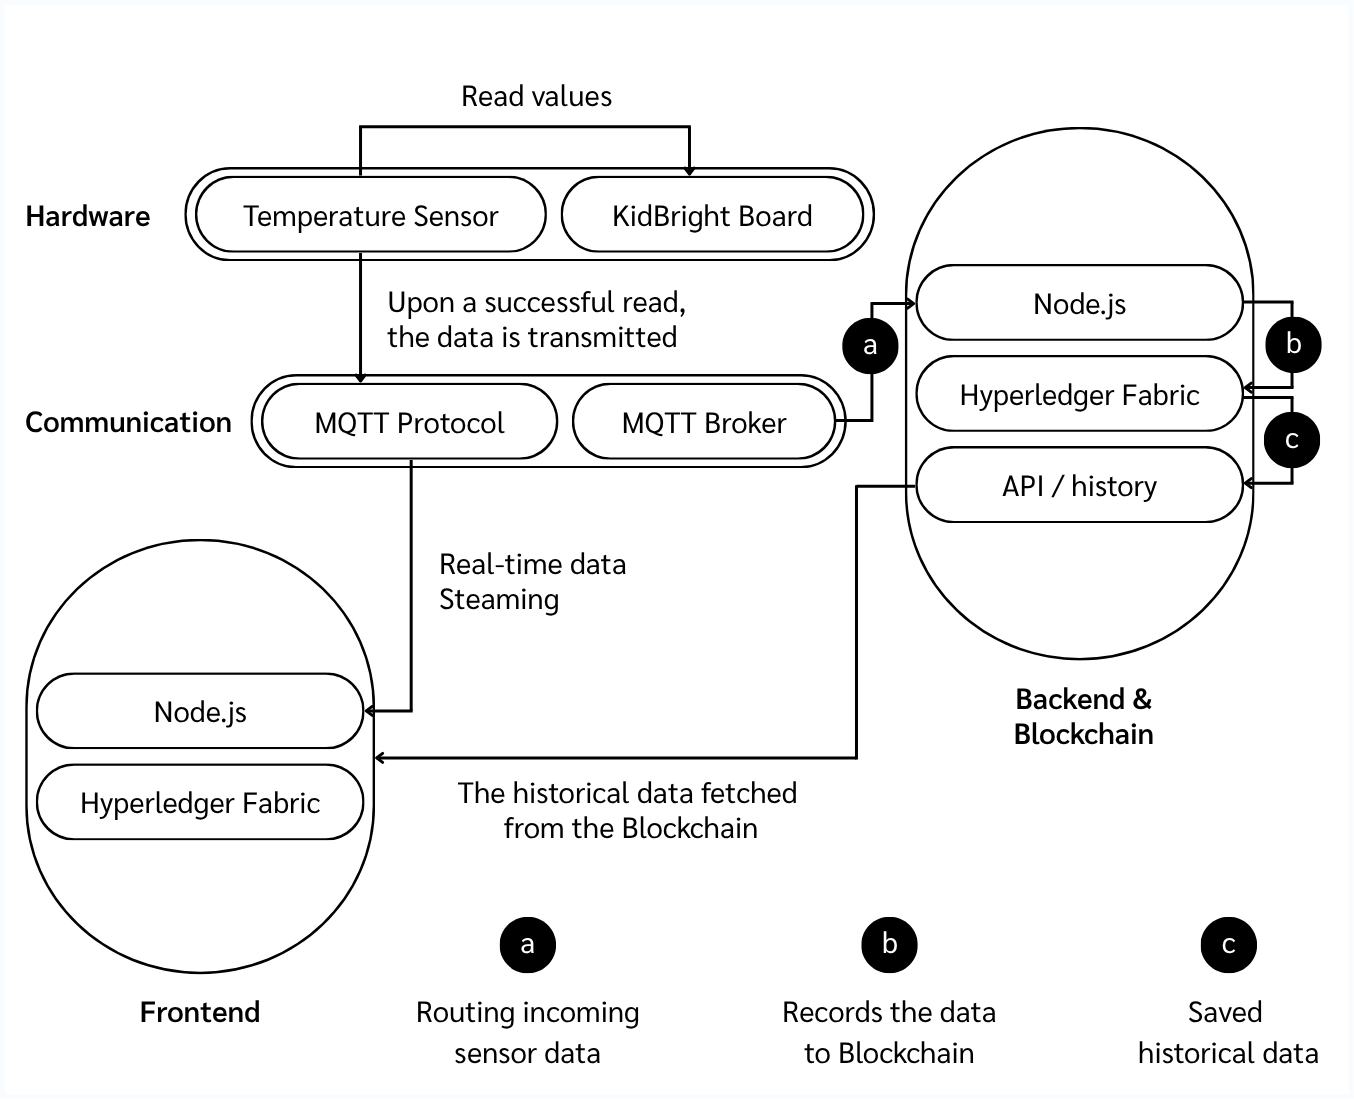
\includegraphics[width=0.9\textwidth]{system arch.png}
    \end{center}
    \caption{การออกแบบสถาปัตยกรรมและการทำงานของระบบ}
    \label{fig:system_arch}
\end{figure}

\section{การออกแบบฮาร์ดแวร์และอุปกรณ์ IoT}
ในส่วนของการตรวจจับข้อมูล อาศัยเซนเซอร์วัดอุณหภูมิที่ติดตั้งไว้ภายในกล่องบรรจุสินค้า เพื่อทำหน้าที่ตรวจวัดและบันทึกค่าอุณหภูมิที่เกิดขึ้นจริงอย่างต่อเนื่องตลอดกระบวนการขนส่ง โดยมีการออกแบบวงจรและลักษณะของอุปกรณ์ดังนี้

\begin{figure}[H]
    \begin{center}
    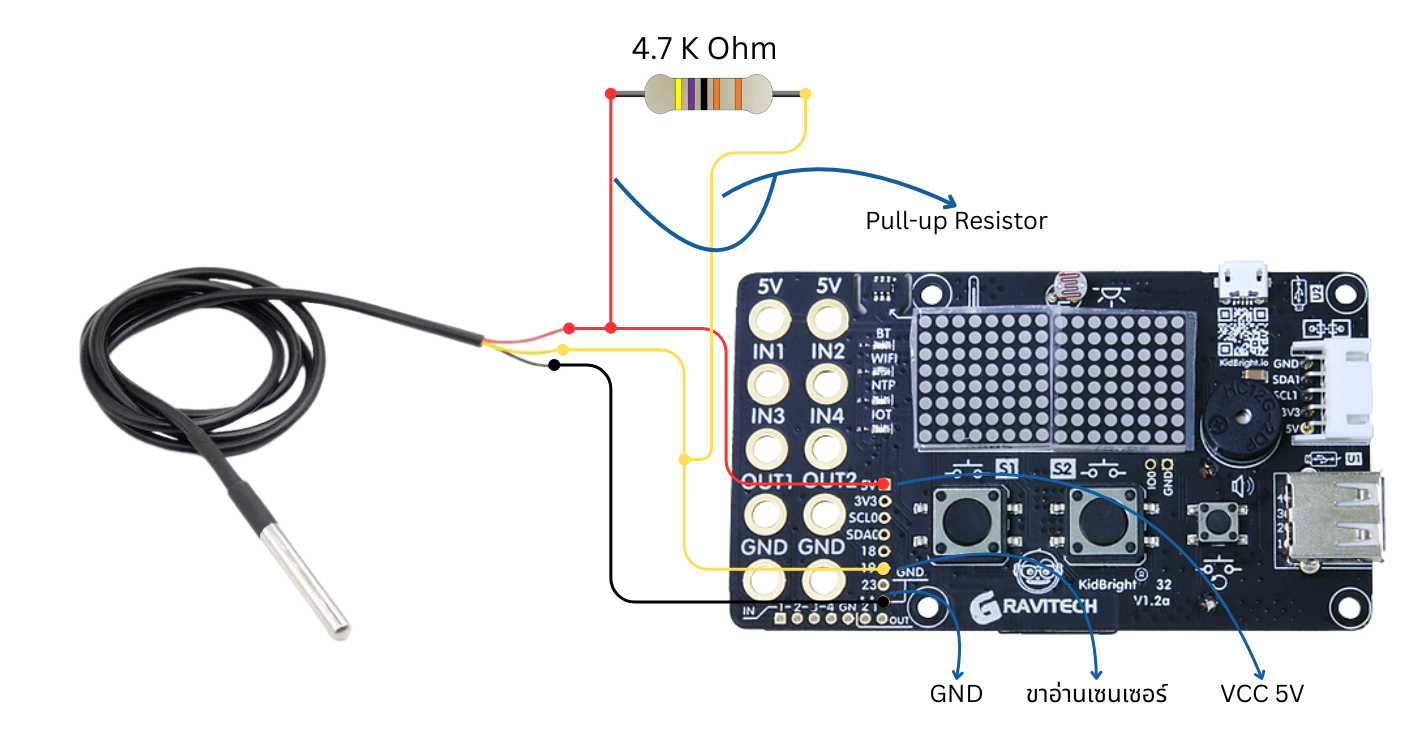
\includegraphics[width=0.8\textwidth]{492 Diagram.png}
    \end{center}
    \caption{แผนผังการต่อวงจรไมโครคอนโทรลเลอร์และเซนเซอร์วัดอุณหภูมิ}
    \label{fig:wiring_diagram}
\end{figure}

\begin{figure}[H]
    \begin{center}
    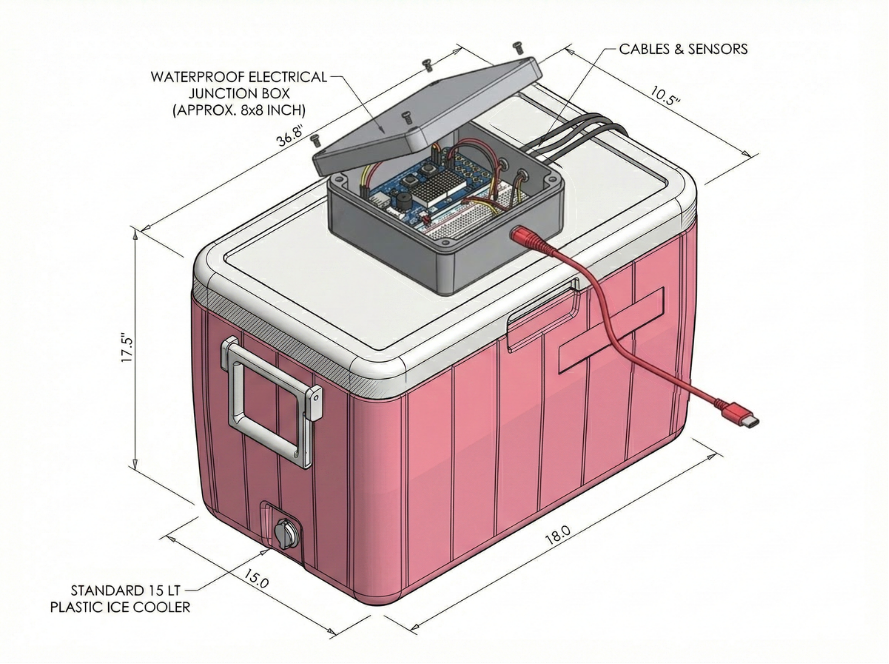
\includegraphics[width=0.8\textwidth]{IoT Box Design.png}
    \end{center}
    \caption{การออกแบบกล่องบรรจุสินค้าและตำแหน่งติดตั้งอุปกรณ์ IoT}
    \label{fig:iot_box}
\end{figure}

\section{ขั้นตอนการดำเนินงานของระบบ}
การทำงานของระบบถูกออกแบบให้ครอบคลุมตั้งแต่ต้นทางจนถึงปลายทางการขนส่ง โดยมีขั้นตอนดังต่อไปนี้:

\subsection{การบันทึกข้อมูลสินค้า}
\begin{itemize}
    \item เจ้าหน้าที่ดำเนินการป้อนข้อมูลที่เกี่ยวข้องกับการขนส่ง เช่น ข้อมูลผู้ส่ง ข้อมูลผู้รับ รายละเอียดของสินค้า และช่วงอุณหภูมิควบคุมที่กำหนด
    \item ระบบจะทำการสร้างรายการขนส่งและออกหมายเลขติดตามพัสดุ เพื่อใช้สำหรับตรวจสอบสถานะของสินค้าตลอดกระบวนการ
\end{itemize}

\subsection{การตรวจสอบและบันทึกอุณหภูมิแบบเรียลไทม์}
\begin{itemize}
    \item อุปกรณ์เซนเซอร์ IoT ที่ติดตั้งบริเวณกล่องบรรจุสินค้า จะทำการวัดค่าอุณหภูมิอย่างต่อเนื่อง และส่งข้อมูลผ่านเครือข่ายอินเทอร์เน็ตไปยัง Amazon EC2 Server
    \item ข้อมูลอุณหภูมิจะถูกส่งผ่านโปรโตคอล MQTT เพื่อนำไปแสดงผล และถูกส่งไปบันทึกลงในระบบบล็อกเชน (Hyperledger Fabric) ผ่าน Smart Contract เพื่อรับประกันความปลอดภัยและป้องกันการแก้ไขข้อมูลย้อนหลัง
    \item ผู้มีส่วนได้ส่วนเสียสามารถติดตามสถานะอุณหภูมิของสินค้าได้แบบเรียลไทม์ผ่านเว็บแอปพลิเคชัน
\end{itemize}

\subsection{การแจ้งเตือนเมื่อพบค่าผิดปกติ}
\begin{itemize}
    \item หากอุณหภูมิของสินค้าสูงหรือต่ำกว่าช่วงที่กำหนด ระบบจะแสดงการแจ้งเตือนบนแพลตฟอร์มเว็บไซต์ทันที
    \item เจ้าหน้าที่หรือผู้ควบคุมระบบสามารถรับทราบปัญหา และดำเนินการแก้ไขสถานการณ์ หรือแจ้งให้ผู้ที่เกี่ยวข้องทราบได้อย่างทันท่วงที เพื่อลดความเสียหายของสินค้า
\end{itemize}

\subsection{การติดตามสถานะและการแสดงผล}
\begin{itemize}
    \item ในระหว่างกระบวนการขนส่ง ระบบจะแสดงผลเฉพาะค่าอุณหภูมิและสถานะปัจจุบันแบบเรียลไทม์บนเว็บแอปพลิเคชัน เพื่อมุ่งเน้นให้ผู้ใช้งานสามารถเฝ้าระวังอุณหภูมิและรับมือกับความผิดปกติได้อย่างทันท่วงที
    \item เมื่อกระบวนการขนส่งเสร็จสมบูรณ์ ระบบจะทำการดึงข้อมูลอุณหภูมิที่ถูกบันทึกไว้ตลอดการเดินทางมาประมวลผล เพื่อแสดงผลในรูปแบบกราฟเชิงเวลา (Time-series Graph) โดยกราฟจะแสดงให้เห็นถึงการเปลี่ยนแปลงของอุณหภูมิตั้งแต่จุดเริ่มต้นการจัดส่งจนถึงจุดหมายปลายทาง พร้อมทั้งสรุปค่าทางสถิติเพื่อให้ผู้ใช้งานสามารถวิเคราะห์ภาพรวมของการขนส่งในรอบนั้น ๆ ได้
\end{itemize}

\subsection{การปิดกระบวนการขนส่งและการตรวจสอบย้อนหลัง}
\begin{itemize}
    \item เมื่อสินค้าถูกจัดส่งถึงปลายทางและผู้รับได้ทำการเซ็นยืนยันการรับสินค้าผ่านระบบเรียบร้อยแล้ว กระบวนการขนส่งจะถือว่าสิ้นสุดอย่างสมบูรณ์ และระบบจะบันทึกสถานะการส่งมอบเป็นขั้นตอนสุดท้าย
    \item หลังจากที่สถานะการขนส่งสิ้นสุดลง ระบบจึงจะเปิดสิทธิ์ให้ผู้ใช้งานสามารถเข้าถึงและตรวจสอบประวัติข้อมูลอุณหภูมิย้อนหลัง ได้ตลอดช่วงระยะเวลาการเดินทางของสินค้า
    \item ในขั้นตอนการตรวจสอบ ระบบจะทำการดึงข้อมูลอุณหภูมิทั้งหมดตั้งแต่เริ่มต้นจนถึงจุดหมายปลายทาง มาเปรียบเทียบกับข้อมูลที่ถูกบันทึกไว้ในระบบบล็อกเชน โดยอ้างอิงจากรอยเวลา (Timestamp) ของแต่ละชุดข้อมูล
    \item กระบวนการนี้เป็นหลักฐานพิสูจน์เชิงประจักษ์ว่า ข้อมูลอุณหภูมิระหว่างการขนส่งไม่เคยถูกดัดแปลงหรือแก้ไข ทำให้สามารถใช้อ้างอิงได้ในกรณีที่เกิดปัญหาหรือข้อพิพาทเกี่ยวกับคุณภาพสินค้า
\end{itemize}

\section{การออกแบบส่วนติดต่อผู้ใช้งาน}
การออกแบบหน้าจอของเว็บแอปพลิเคชันถูกพัฒนาขึ้นเพื่อให้ผู้ใช้งานสามารถโต้ตอบกับระบบได้อย่างสะดวกและมีประสิทธิภาพ โดยแบ่งหมวดหมู่การเข้าถึงออกเป็น 4 ส่วนหลัก ได้แก่ หน้าหลัก (Main) ส่วนการยืนยันตัวตน (Auth) ส่วนของผู้ใช้งานทั่วไป (User) และส่วนของผู้ดูแลระบบ (Admin) โดยมีรายละเอียดหน้าจอดังต่อไปนี้

\subsection{หน้าหลัก}
ในส่วนนี้เป็นหน้าต่างแรกสำหรับผู้ใช้งานทุกคนที่เข้ามาสู่แพลตฟอร์ม ประกอบด้วย:

\vspace{1em}
\begin{minipage}{\linewidth}
\noindent \textbf{1. หน้าแรก} \\
หน้าหลักของเว็บไซต์ที่แสดงข้อมูลเบื้องต้นและภาพรวมของบริการ
\begin{figure}[H]
    \centering
    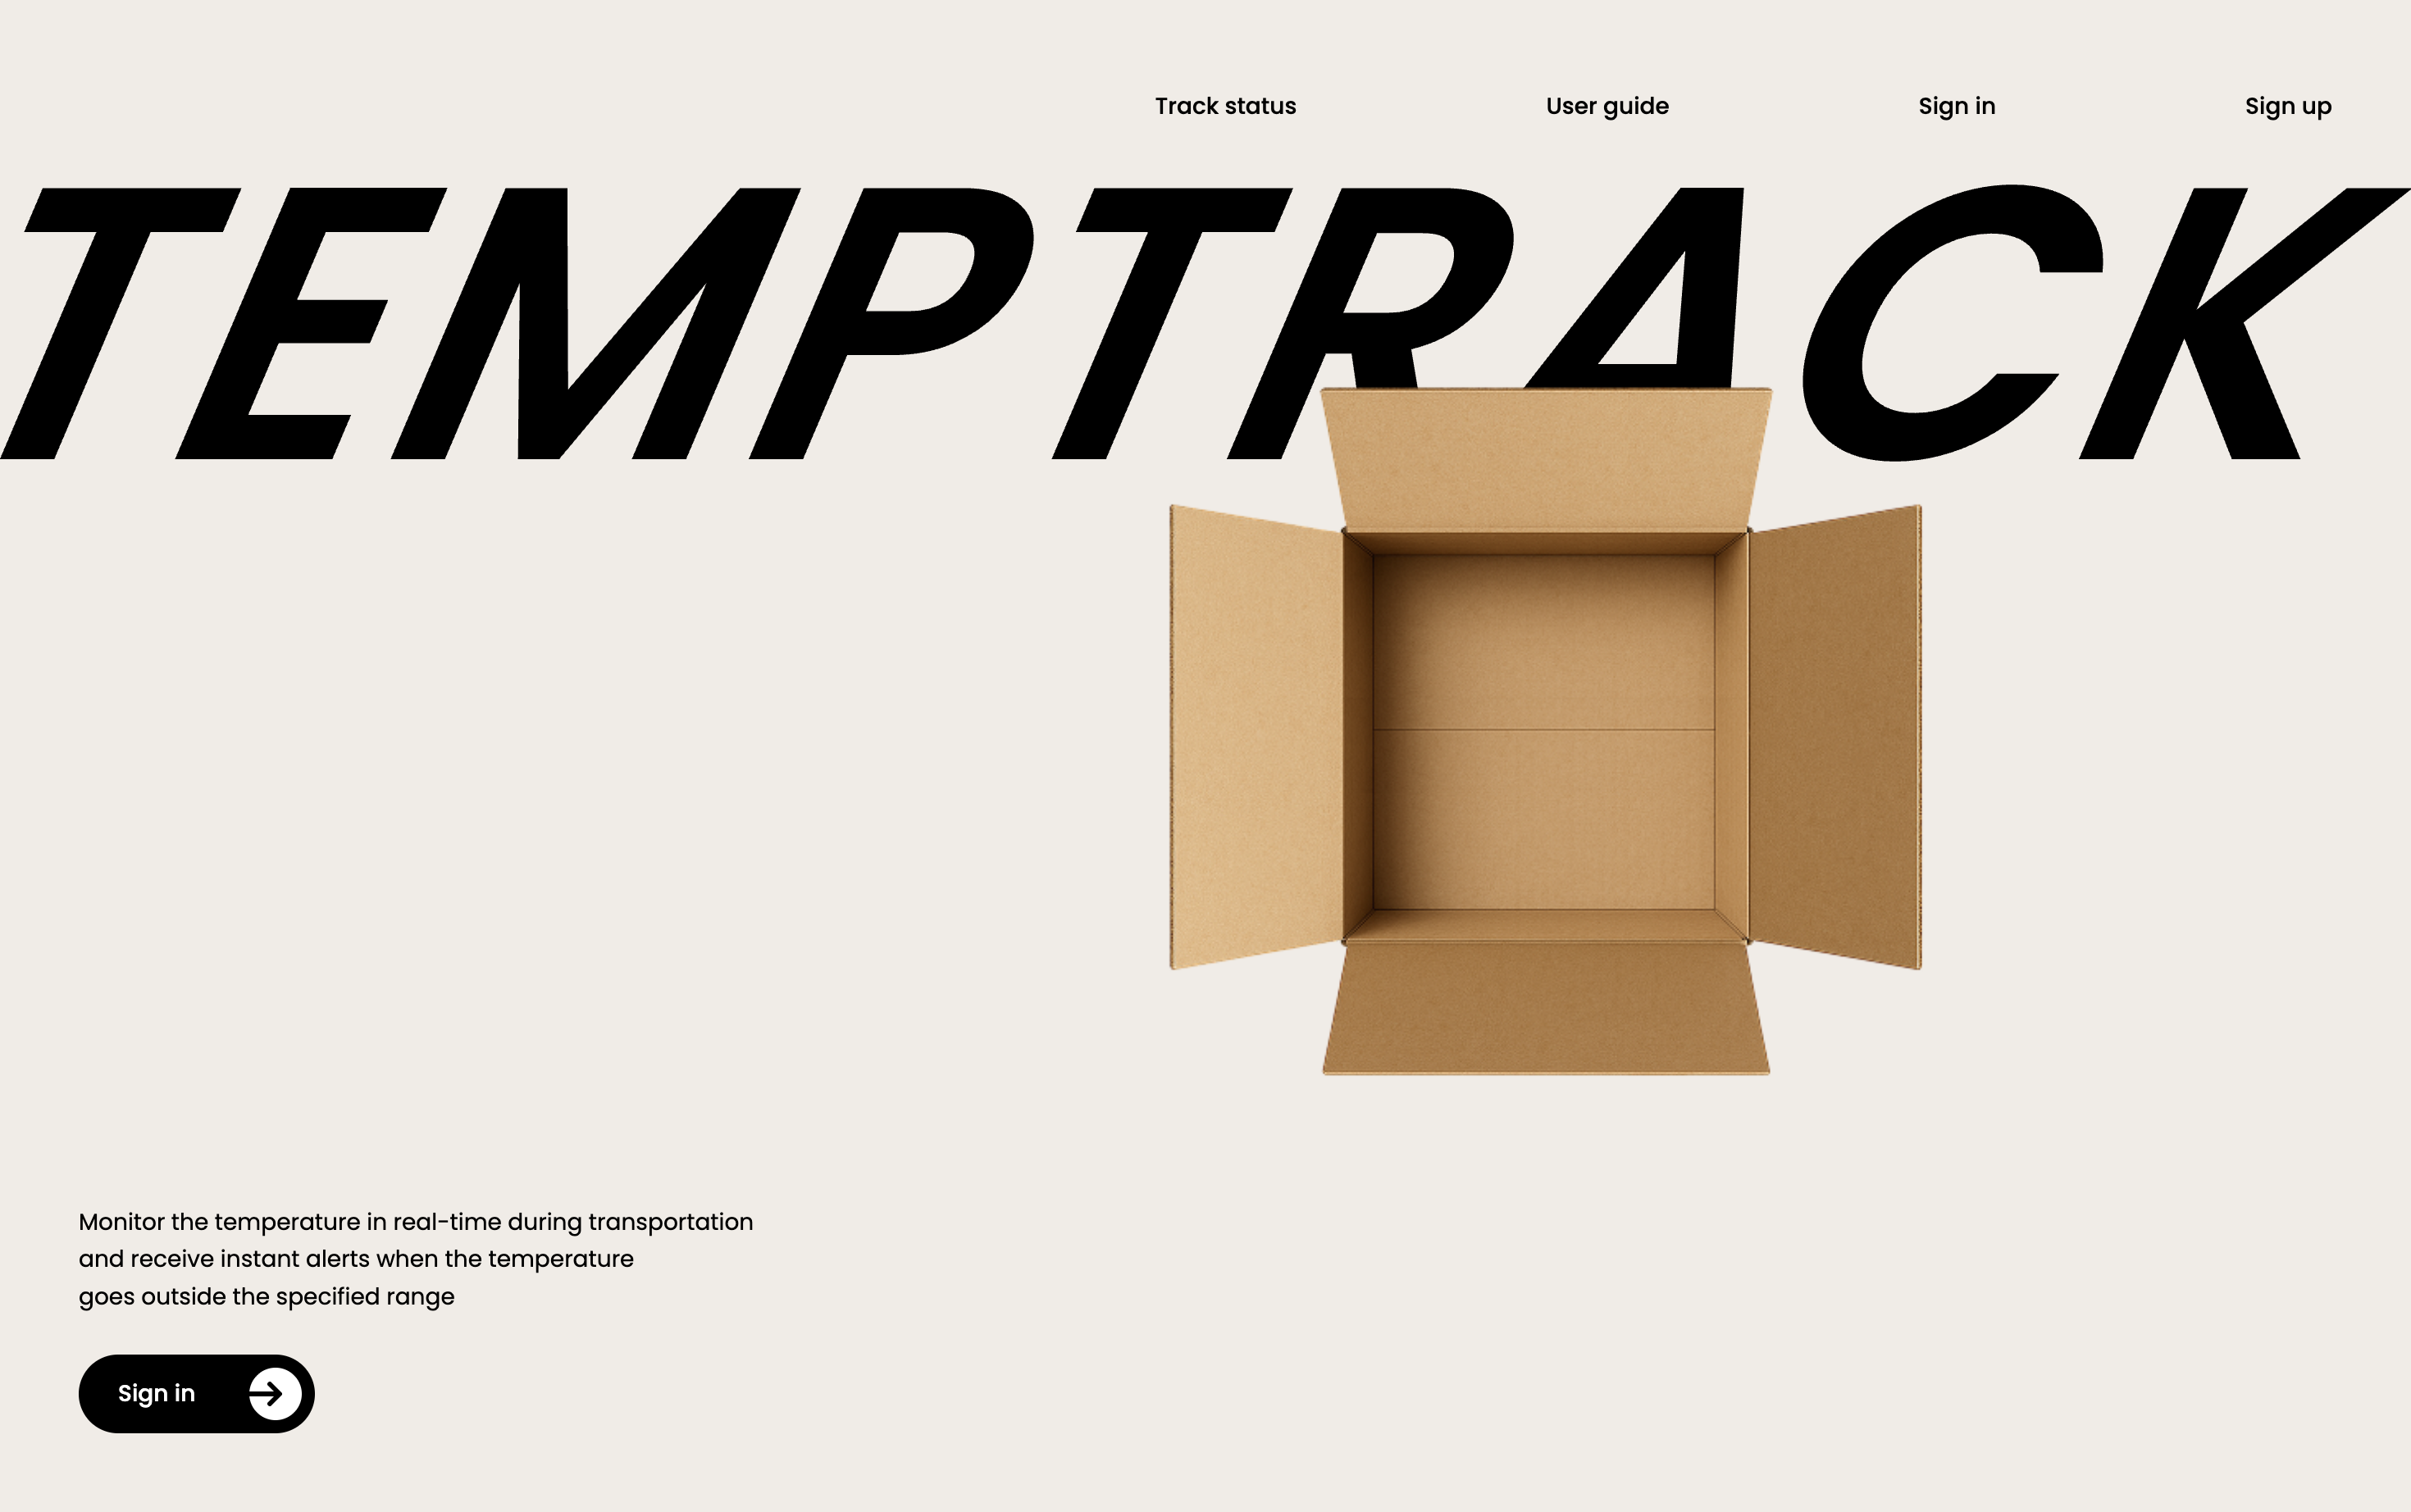
\includegraphics[width=0.8\textwidth]{home.png}
    \caption{หน้าแรก}
    \label{fig:ui_home}
\end{figure}
\end{minipage}

\vspace{1em}
\begin{minipage}{\linewidth}
\noindent \textbf{2. หน้าคู่มือการใช้งาน} \\
อธิบายวิธีการใช้งานแพลตฟอร์มและฟีเจอร์ต่าง ๆ เพื่ออำนวยความสะดวกแก่ผู้ใช้ใหม่
\begin{figure}[H]
    \centering
    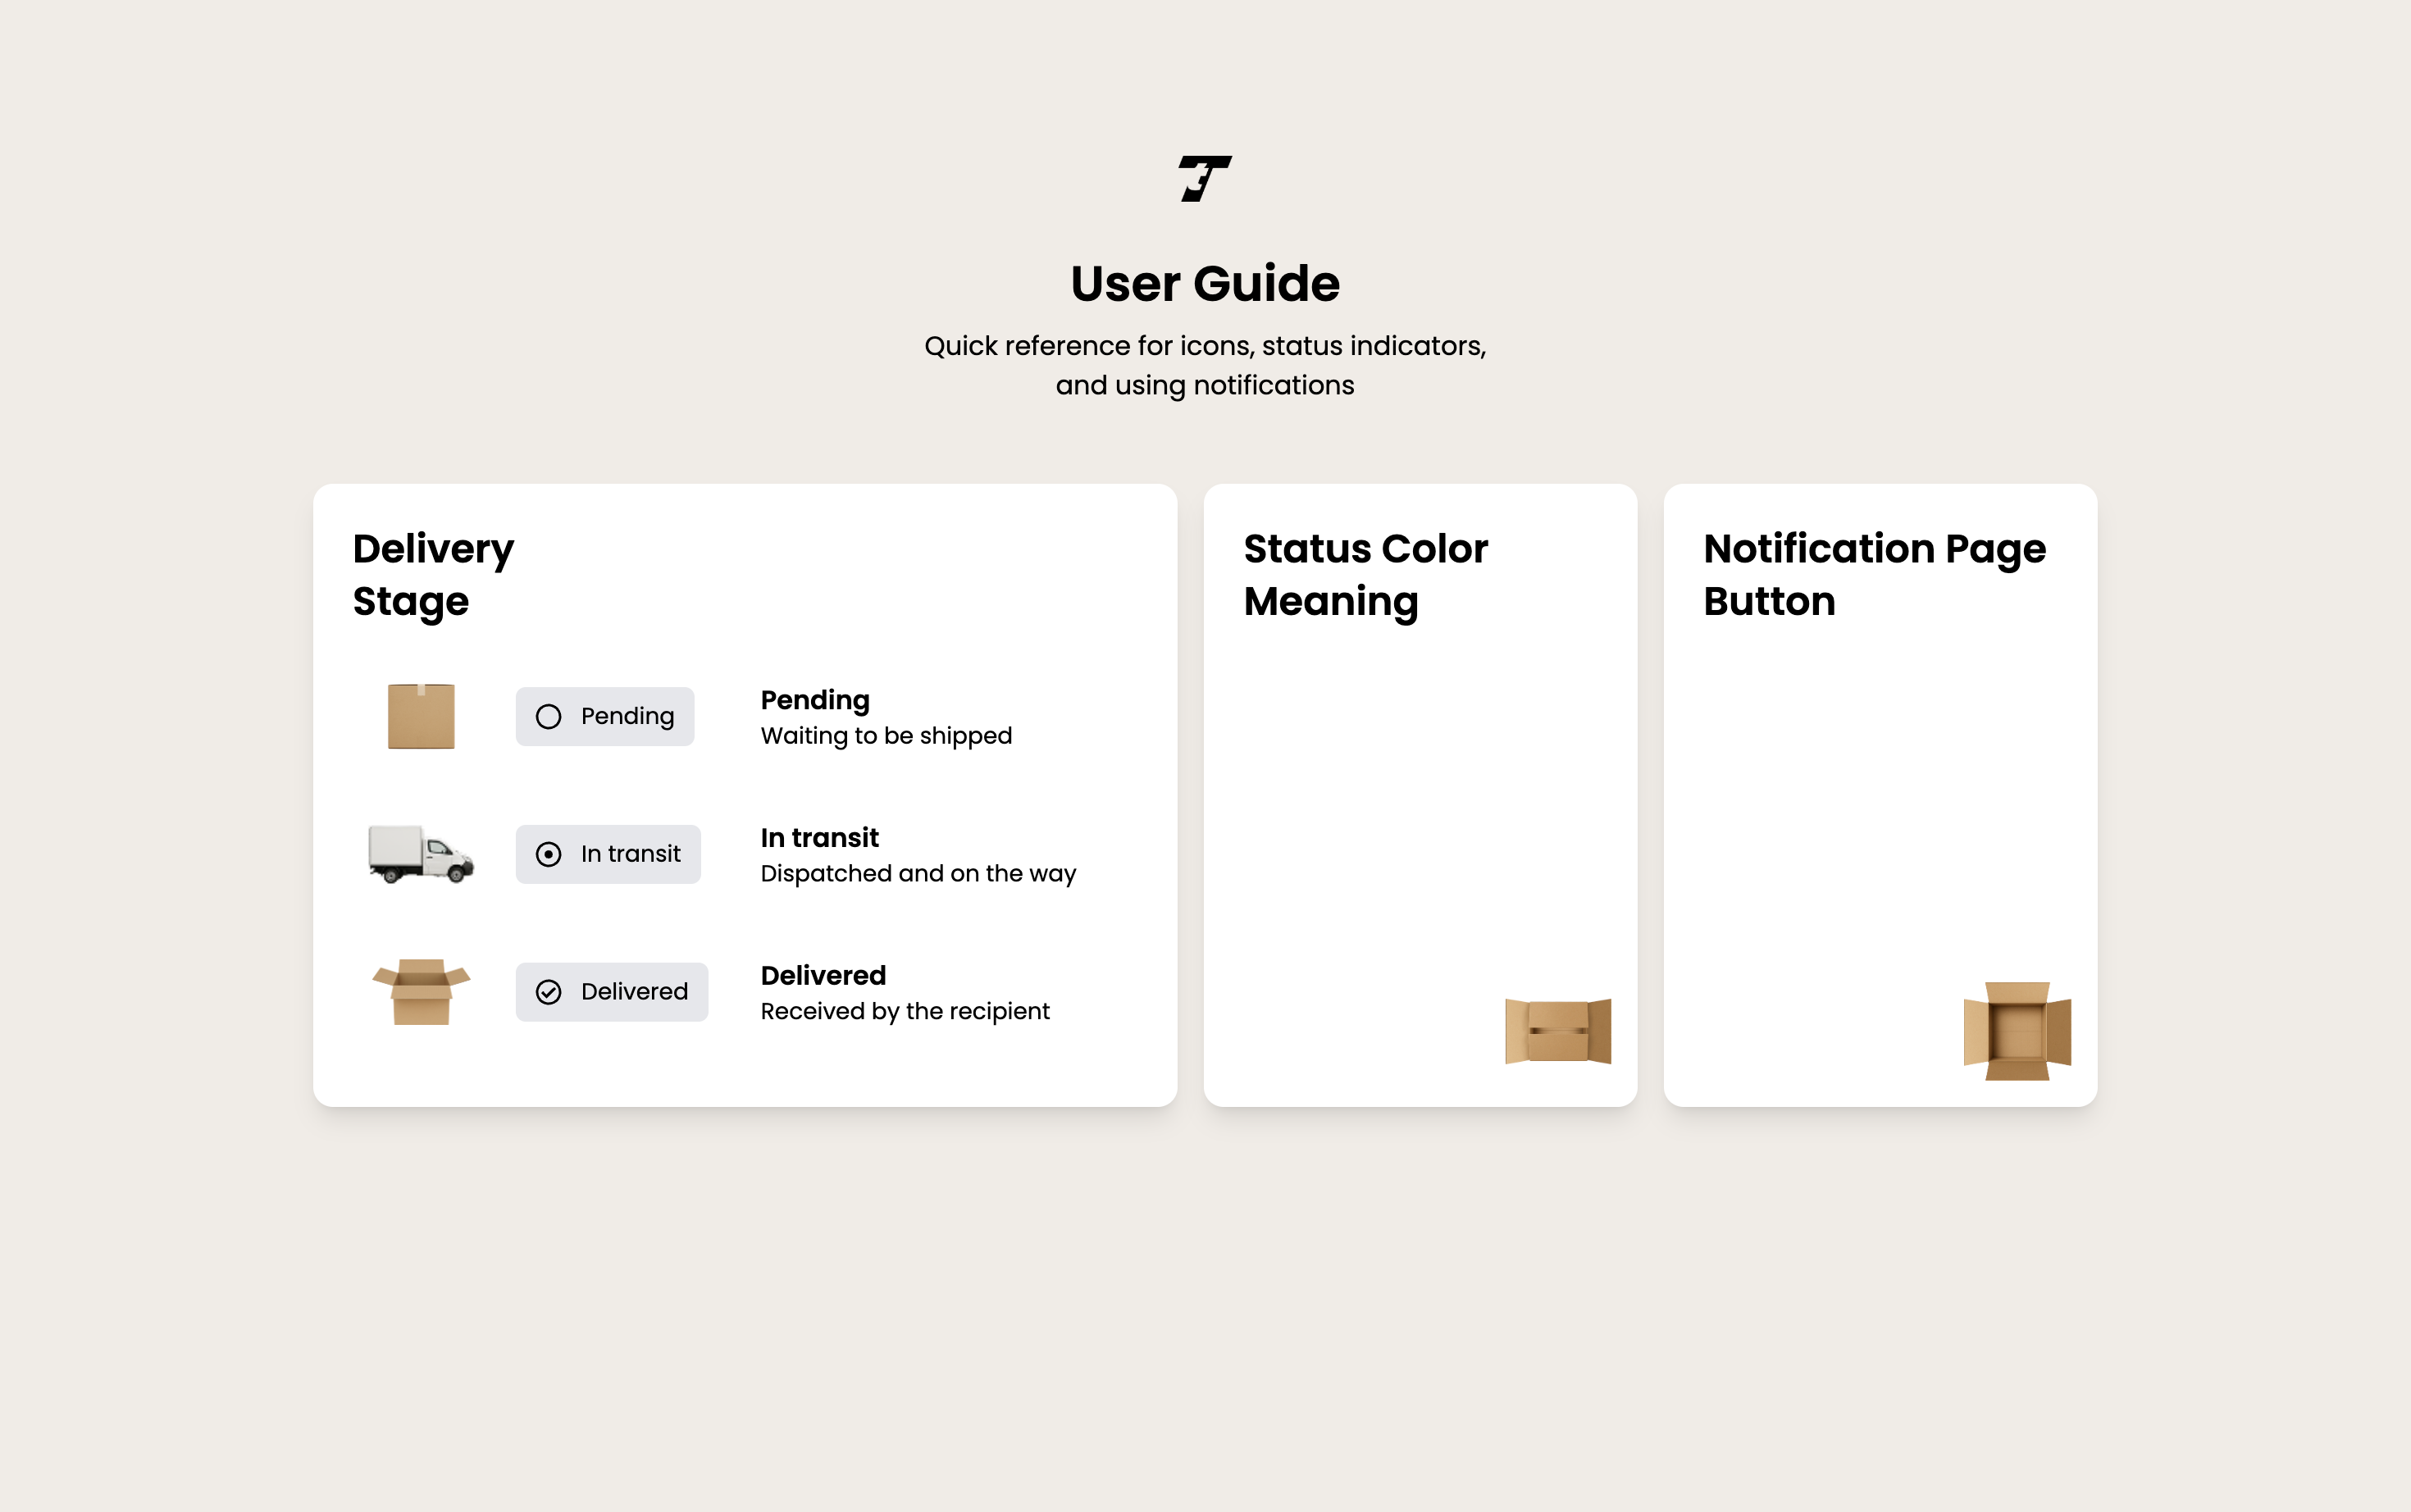
\includegraphics[width=0.8\textwidth]{userguide.png}
    \caption{หน้าคู่มือการใช้งาน}
    \label{fig:ui_guide}
\end{figure}
\end{minipage}


\subsection{ส่วนการยืนยันตัวตน}
ระบบรักษาความปลอดภัยและการเข้าถึงบัญชีผู้ใช้ ประกอบด้วย:

\vspace{1em}
\begin{minipage}{\linewidth}
\noindent \textbf{1. หน้าเข้าสู่ระบบ} \\
สำหรับให้ผู้ใช้งานทั่วไปและผู้ดูแลระบบทำการยืนยันตัวตนเพื่อเข้าสู่ระบบ
\begin{figure}[H]
    \centering
    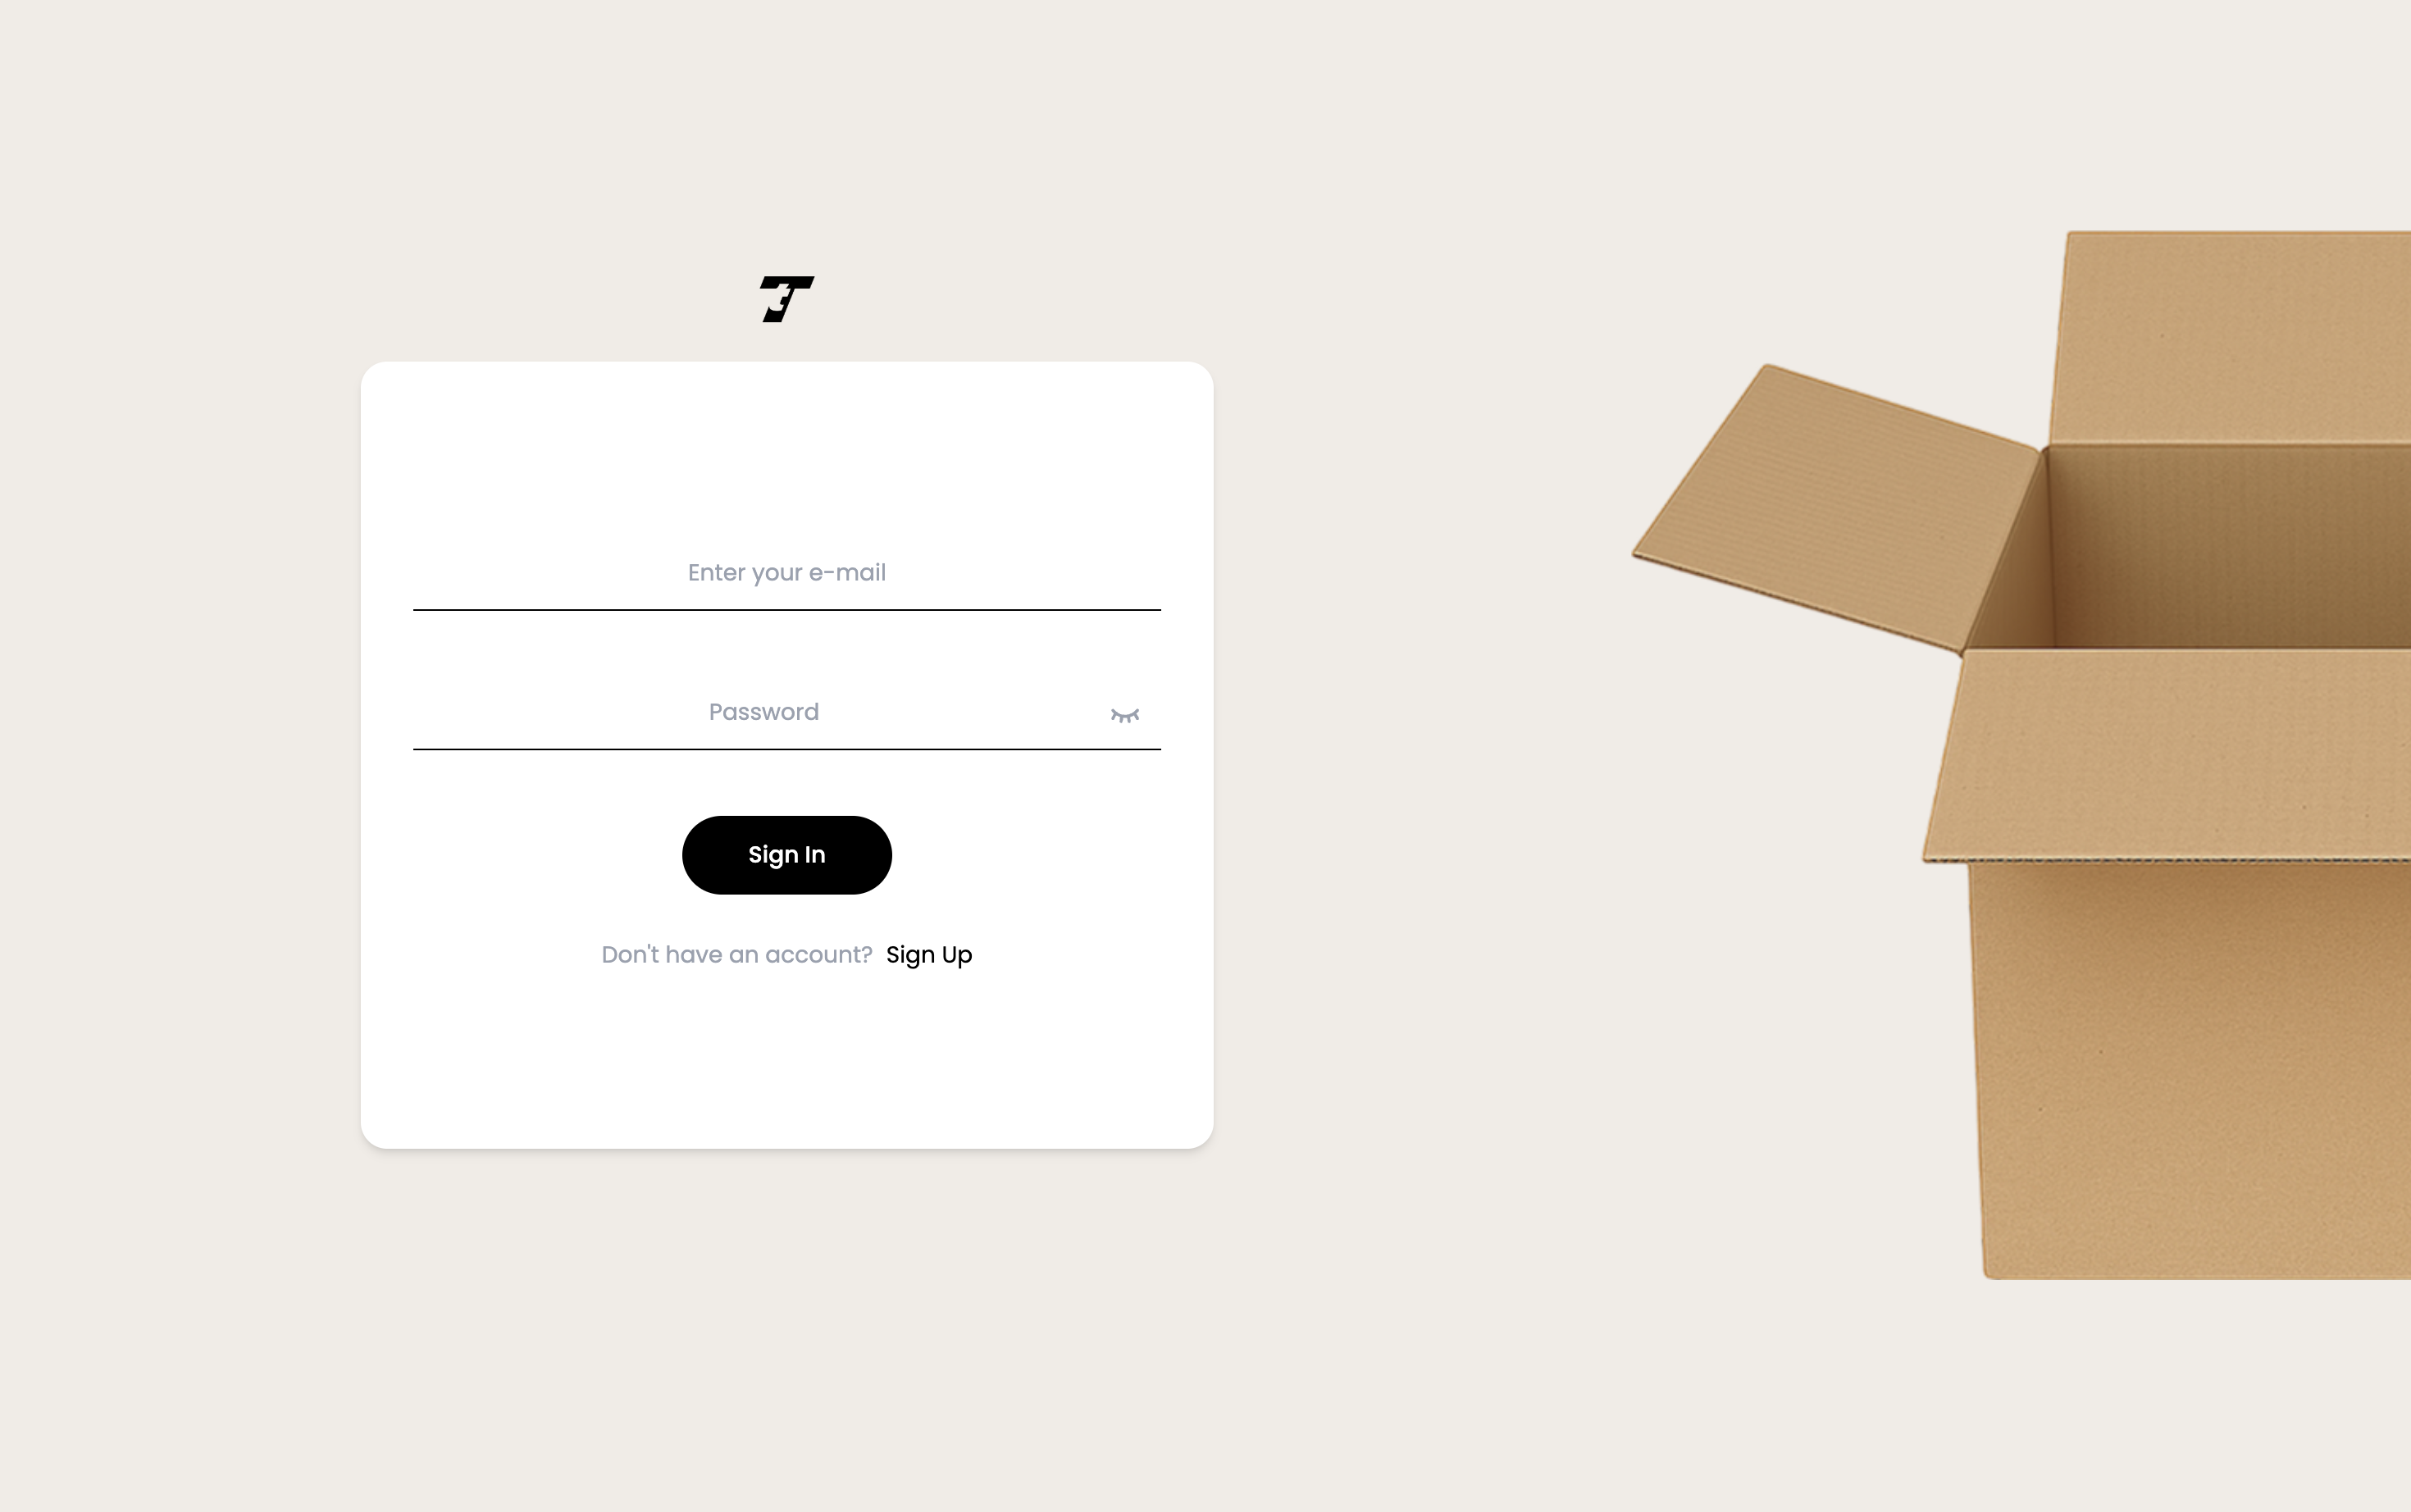
\includegraphics[width=0.8\textwidth]{signin.png}
    \caption{หน้าเข้าสู่ระบบ}
    \label{fig:ui_signin}
\end{figure}
\end{minipage}

\vspace{1em}
\begin{minipage}{\linewidth}
\noindent \textbf{2. หน้าสมัครสมาชิก} \\
สำหรับให้ผู้ใช้งานใหม่ทำการลงทะเบียนและสร้างบัญชีผู้ใช้
\begin{figure}[H]
    \centering
    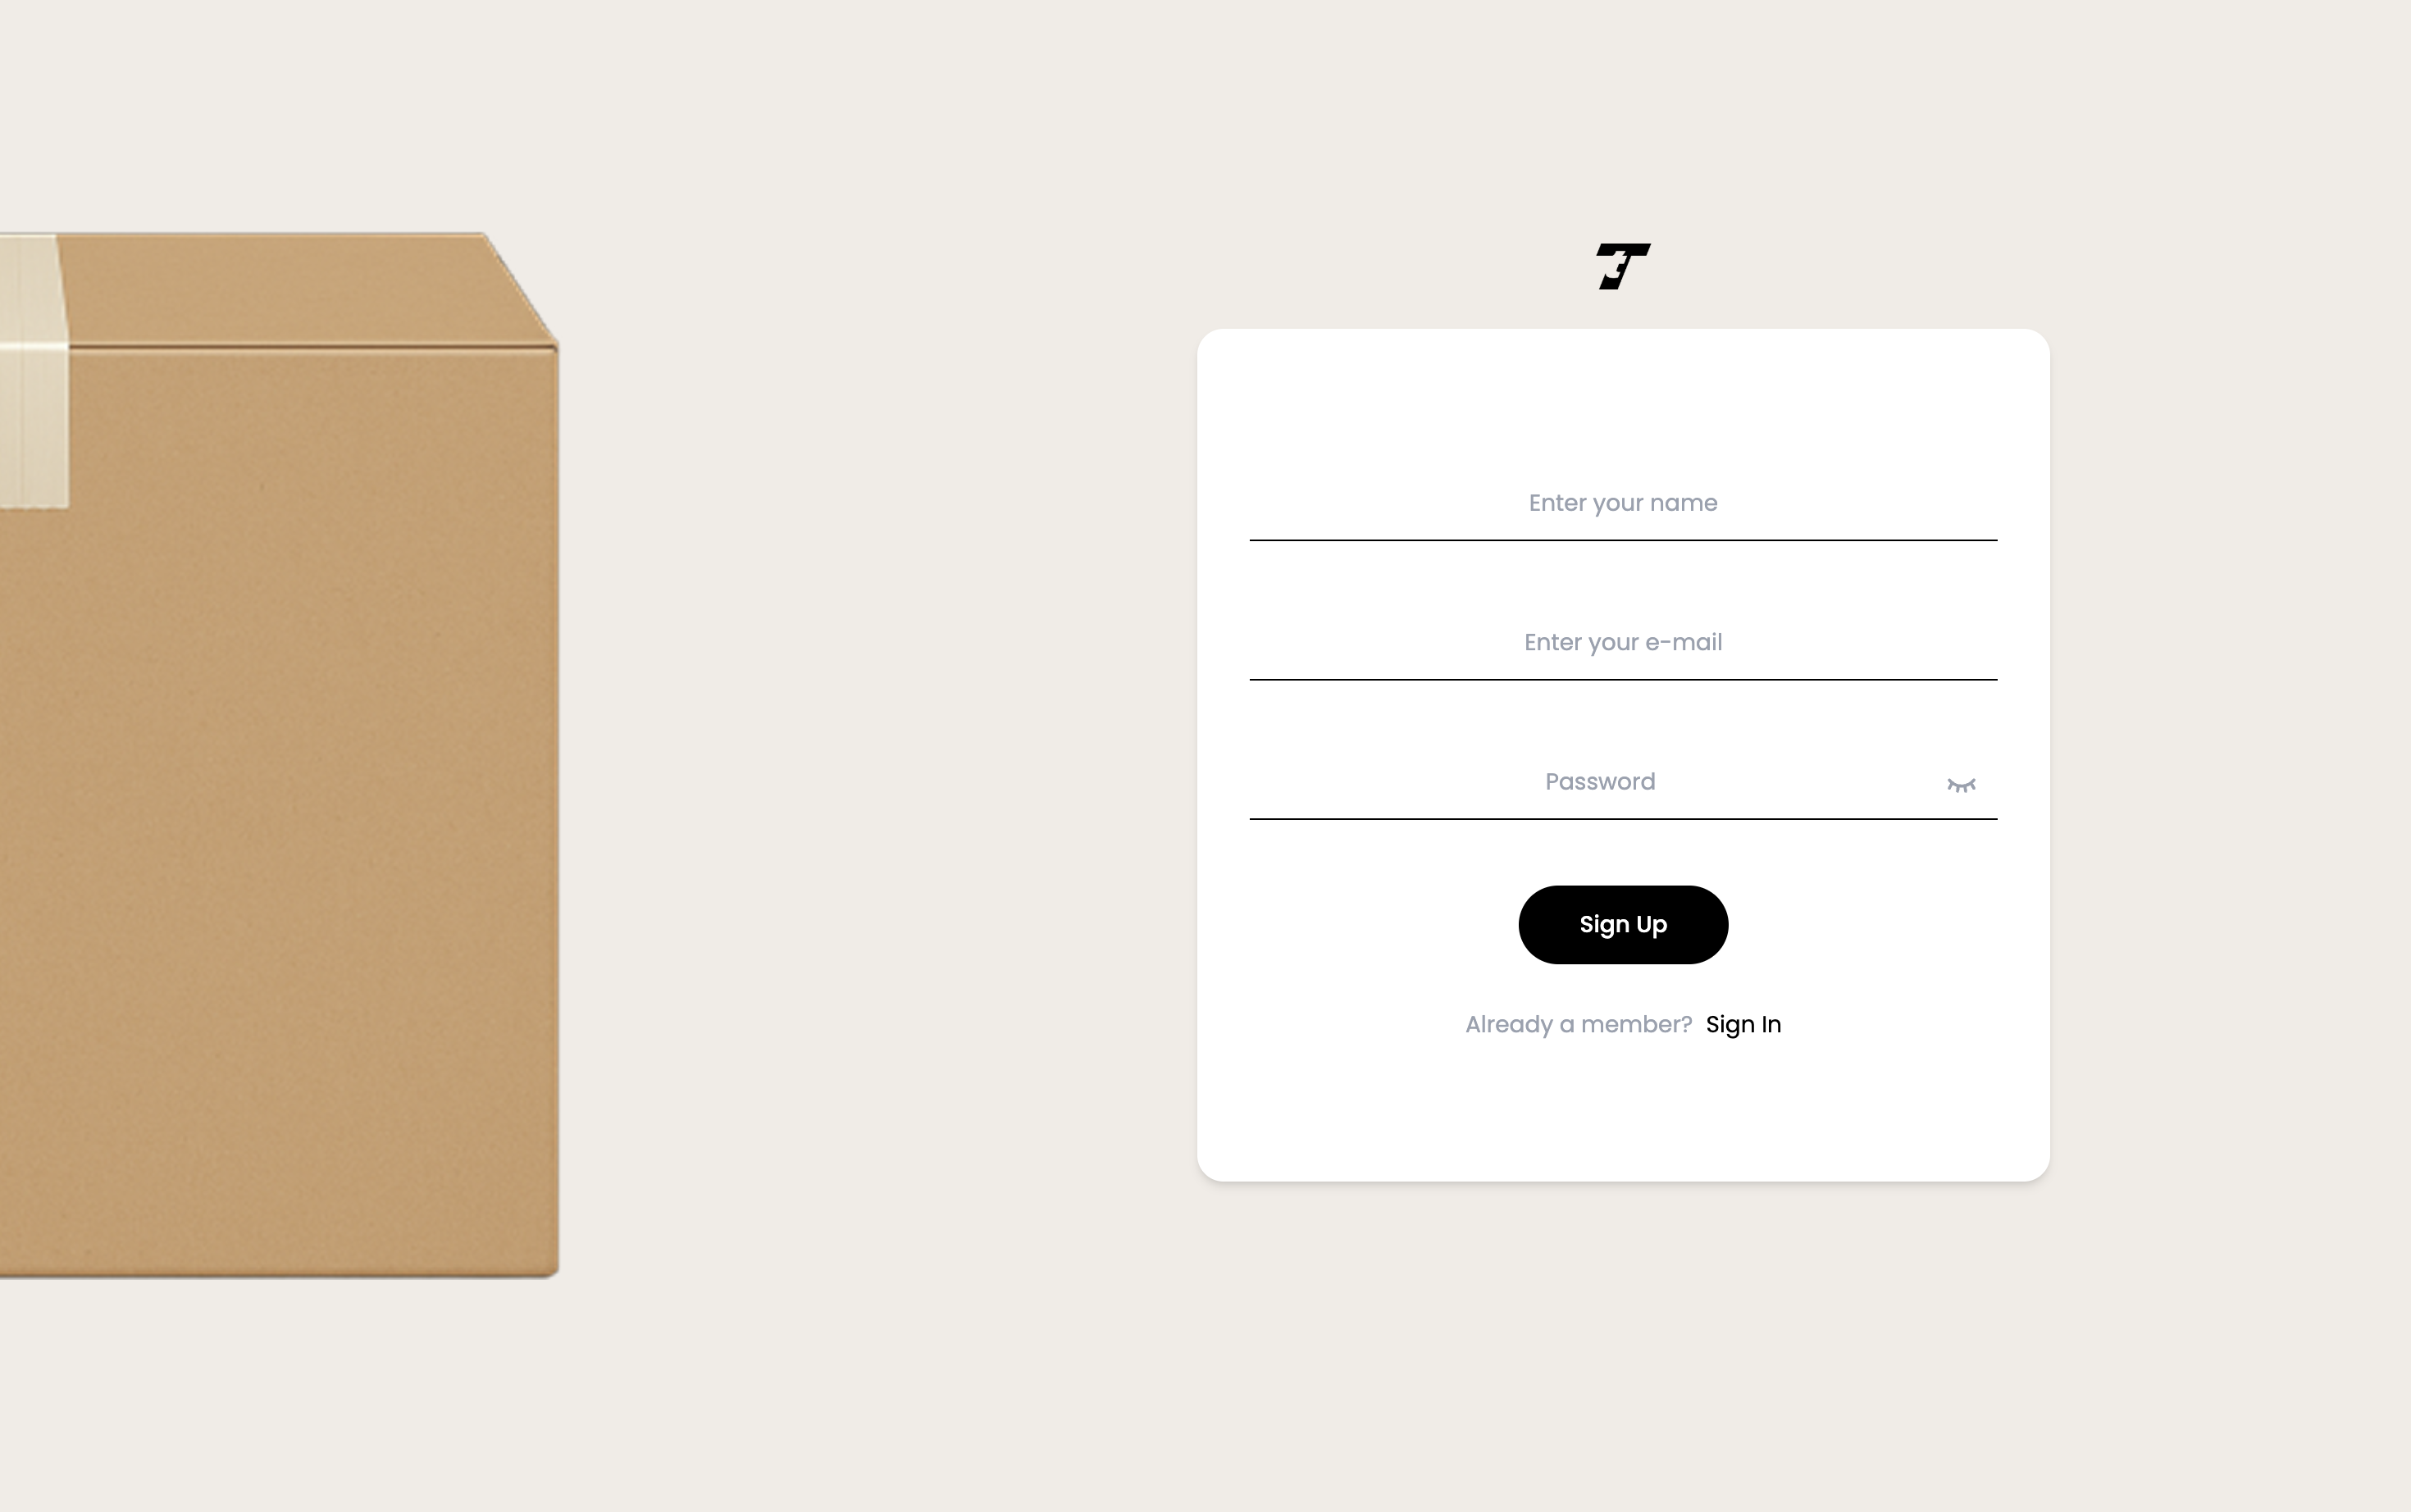
\includegraphics[width=0.8\textwidth]{signup.png}
    \caption{หน้าสมัครสมาชิก}
    \label{fig:ui_signup}
\end{figure}
\end{minipage}


\subsection{ส่วนของผู้ใช้งานทั่วไป}
หมวดหมู่นี้ถูกออกแบบมาเพื่อรองรับผู้ใช้งานใน 2 บทบาทหลัก ได้แก่ \textbf{ผู้ส่งพัสดุ (Sender)} ซึ่งเป็นผู้เดียวที่มีสิทธิ์ในการกรอกและจัดการข้อมูลการจัดส่ง และ \textbf{ผู้ใช้งานทั่วไปหรือผู้รับพัสดุ (Recipient)} ที่เน้นการติดตามสถานะและตรวจสอบความถูกต้อง โดยมีหน้าต่างการทำงานดังนี้:

\vspace{1em}
\begin{minipage}{\linewidth}
\noindent \textbf{1. หน้ากรอกข้อมูลผู้ส่ง} \\
สำหรับให้ \textbf{ผู้ส่งพัสดุ} บันทึกข้อมูลส่วนตัวและที่อยู่ของตนเอง \textit{(ผู้ใช้งานทั่วไปในบทบาทอื่นจะไม่สามารถกรอกข้อมูลในส่วนนี้ได้)}
\begin{figure}[H]
    \centering
    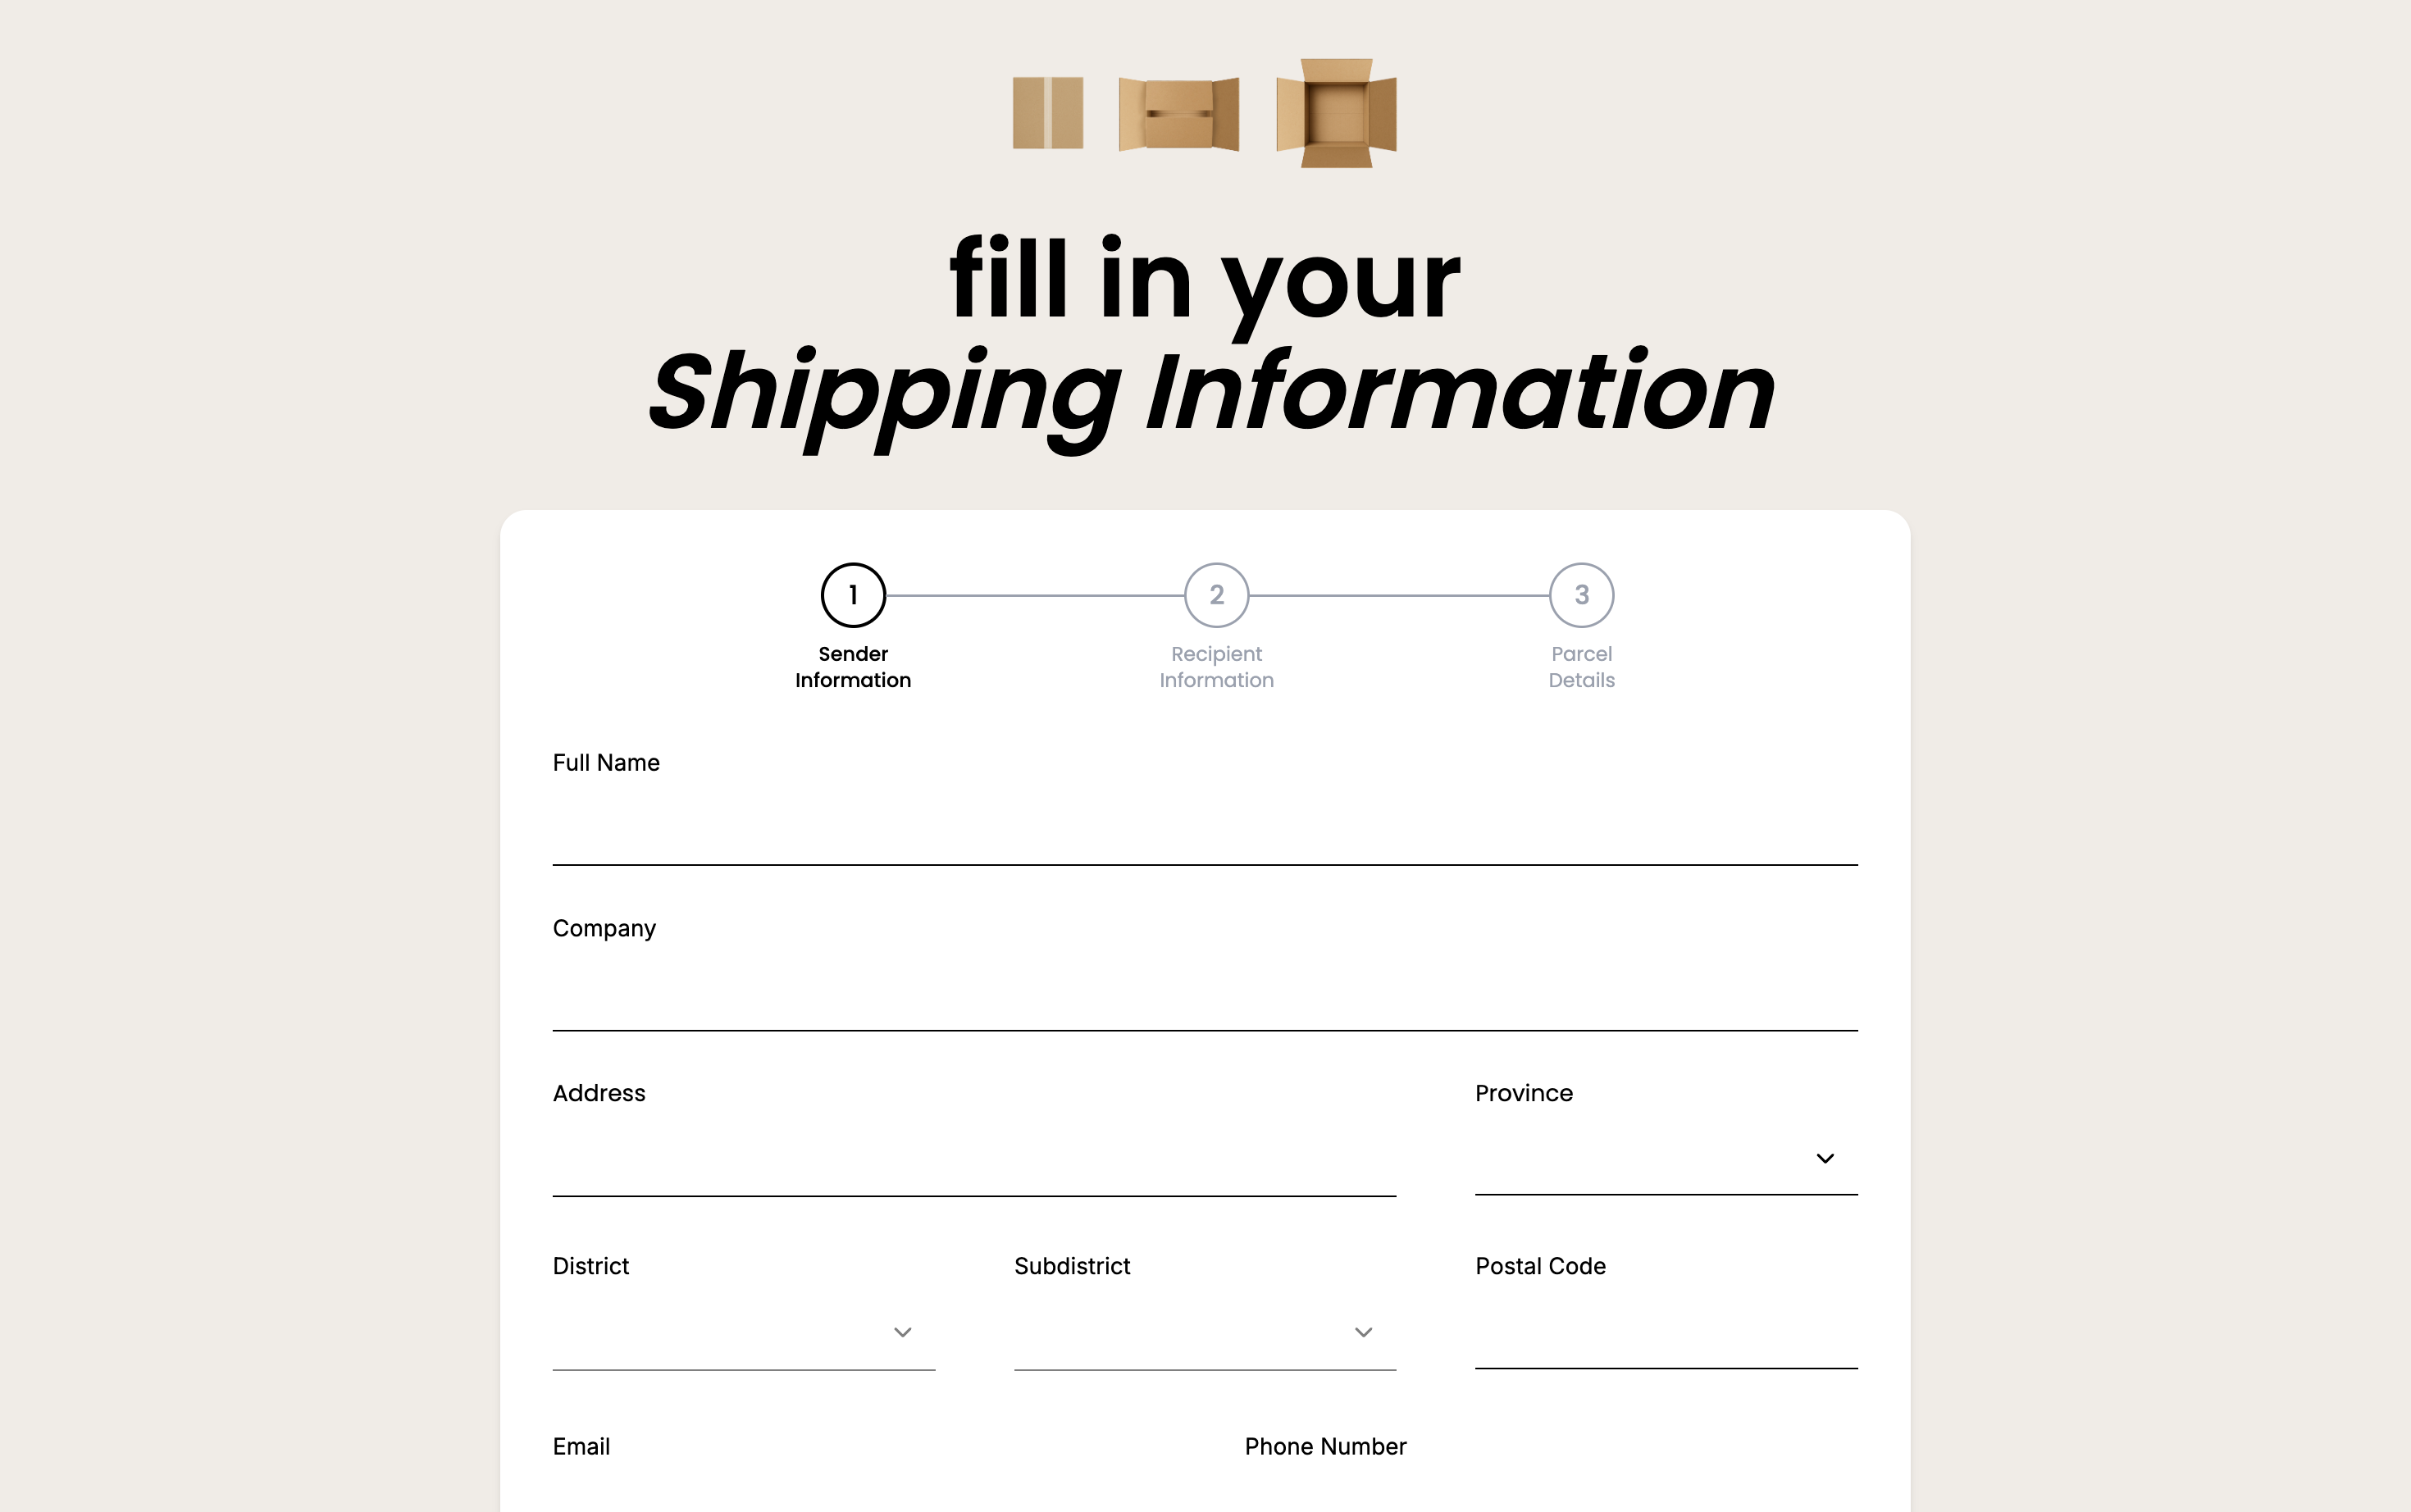
\includegraphics[width=0.8\textwidth]{fillsenderaddress.png}
    \caption{หน้ากรอกข้อมูลผู้ส่ง}
    \label{fig:ui_user_sender}
\end{figure}
\end{minipage}

\vspace{1em}
\begin{minipage}{\linewidth}
\noindent \textbf{2. หน้ากรอกรายละเอียดพัสดุ} \\
สำหรับให้ \textbf{ผู้ส่งพัสดุ} ระบุข้อมูลสำคัญของสินค้า เช่น น้ำหนัก ขนาด และช่วงอุณหภูมิควบคุมที่ต้องการ
\begin{figure}[H]
    \centering
    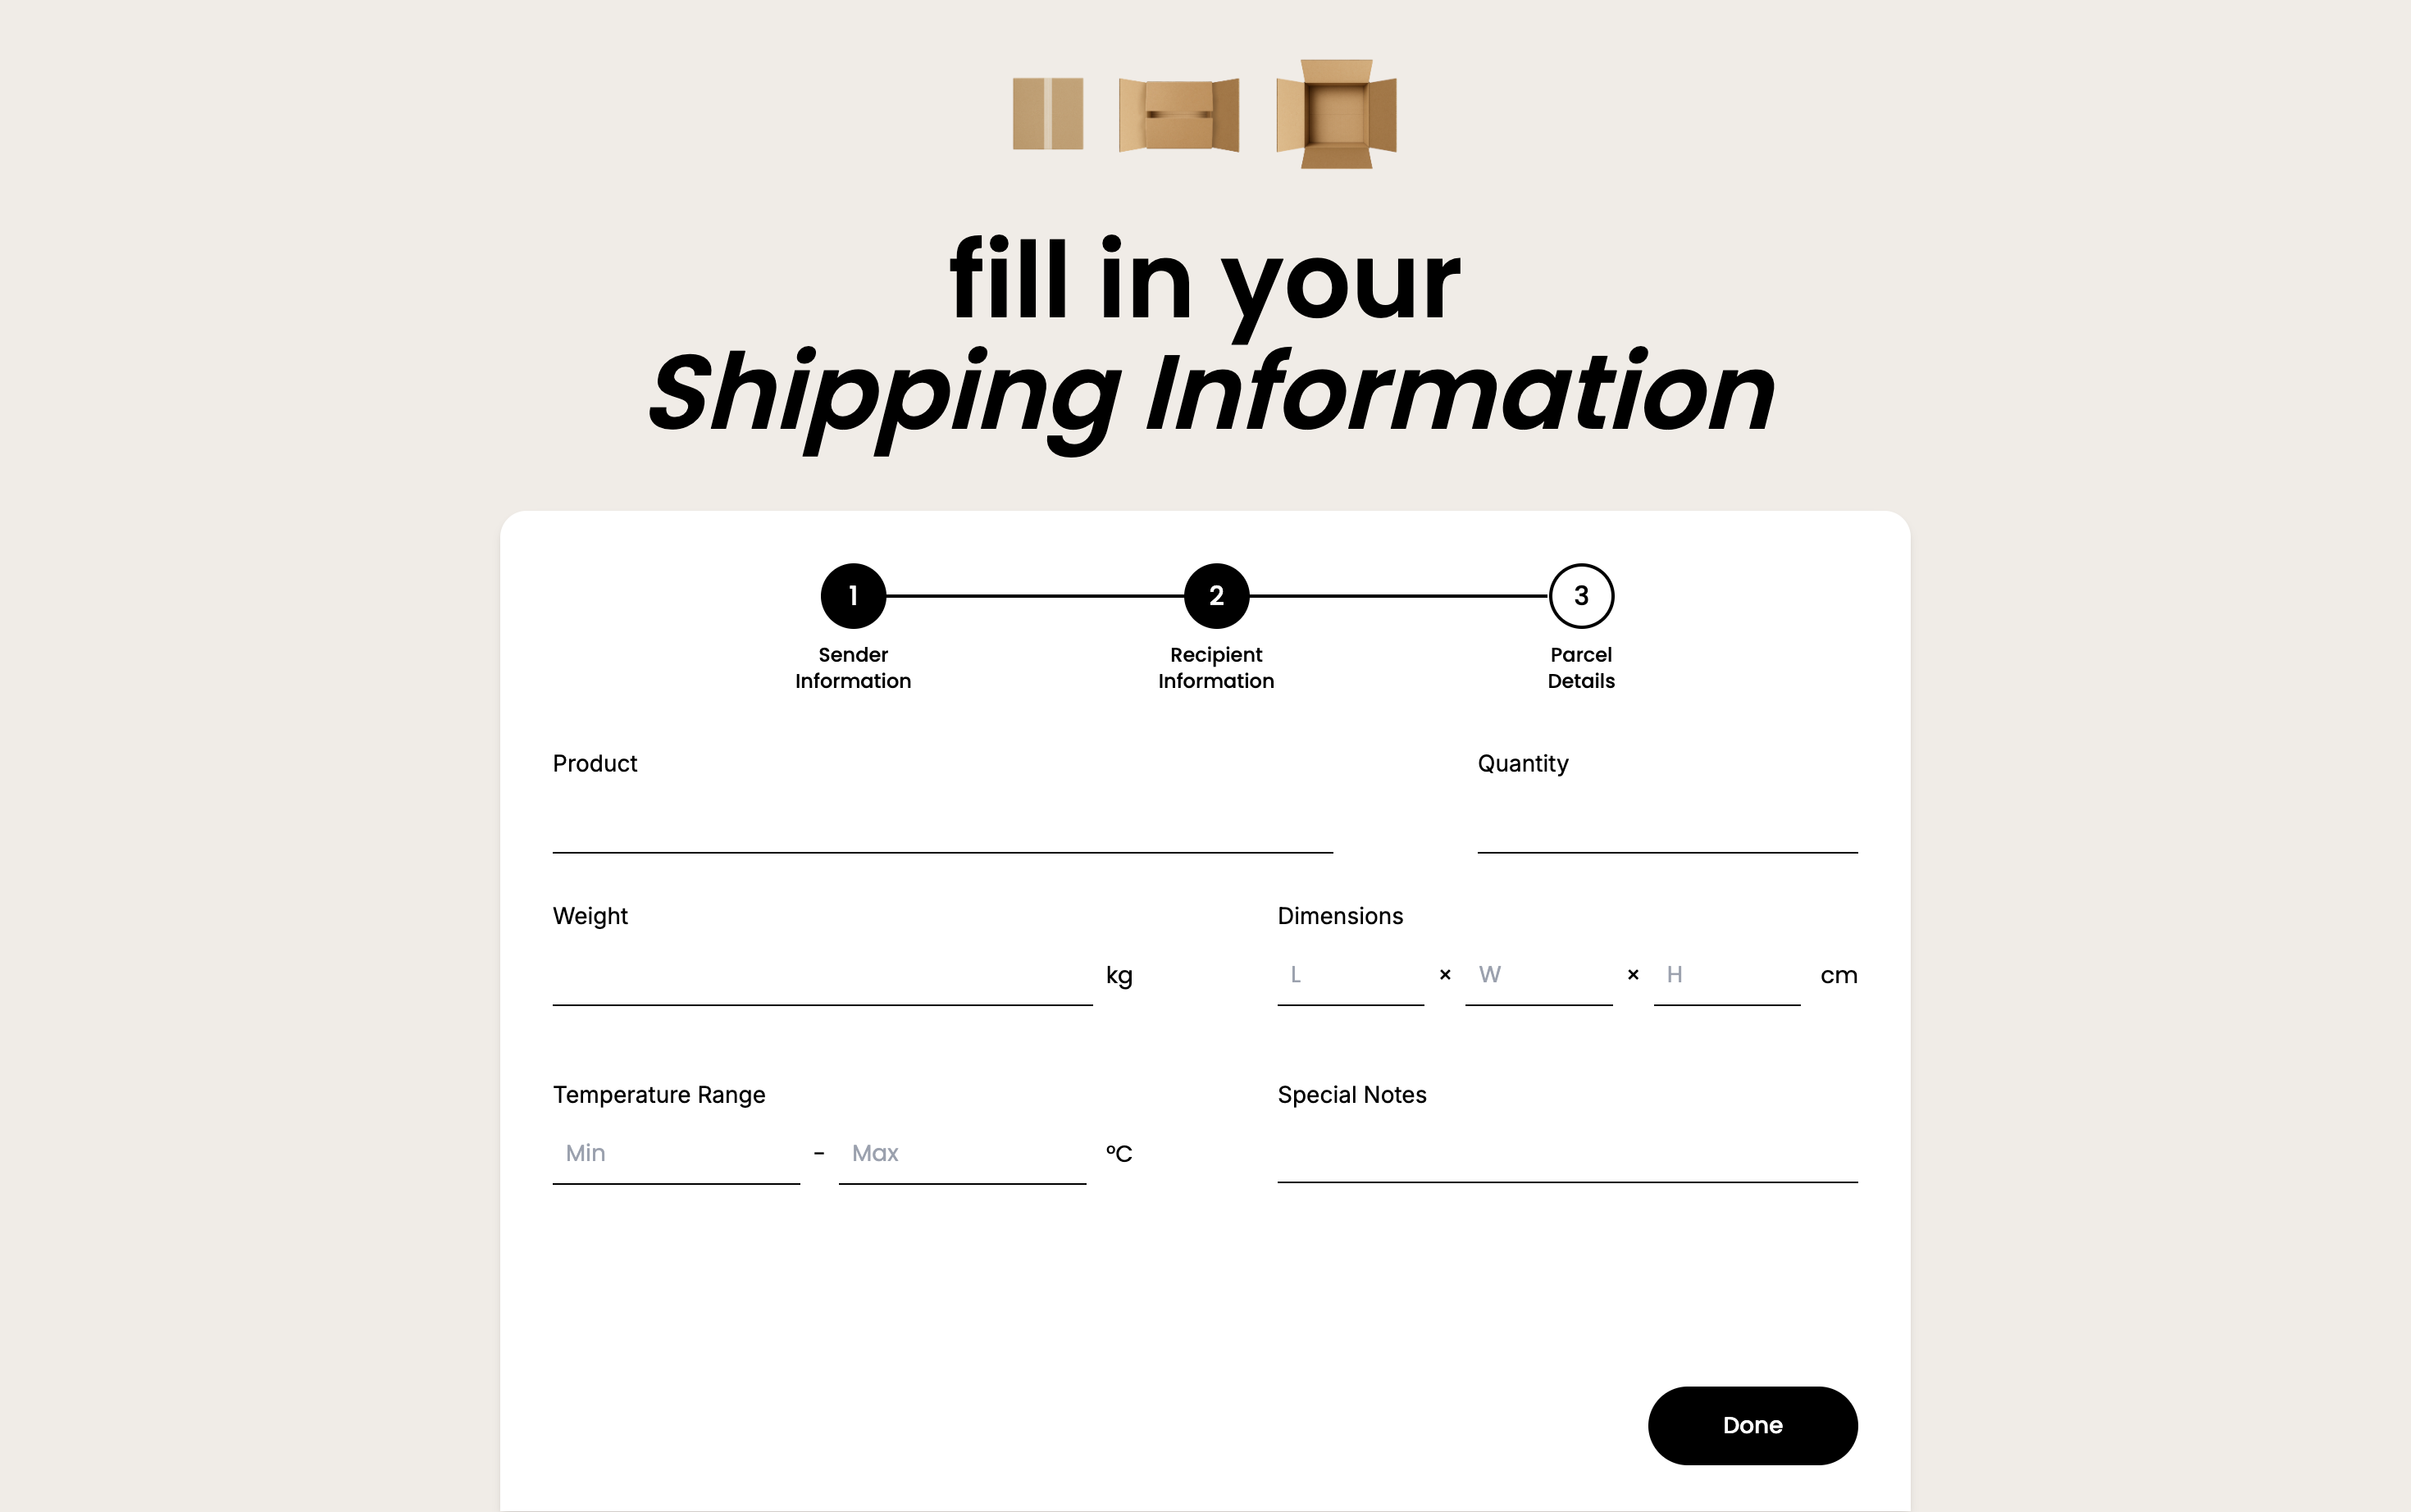
\includegraphics[width=0.8\textwidth]{fillparceldetail.png}
    \caption{หน้ากรอกรายละเอียดพัสดุ}
    \label{fig:ui_user_parcel}
\end{figure}
\end{minipage}

\vspace{1em}
\begin{minipage}{\linewidth}
\noindent \textbf{3. หน้ากรอกข้อมูลผู้รับ} \\
สำหรับให้ \textbf{ผู้ส่งพัสดุ} บันทึกที่อยู่และช่องทางการติดต่อของปลายทาง
\begin{figure}[H]
    \centering
    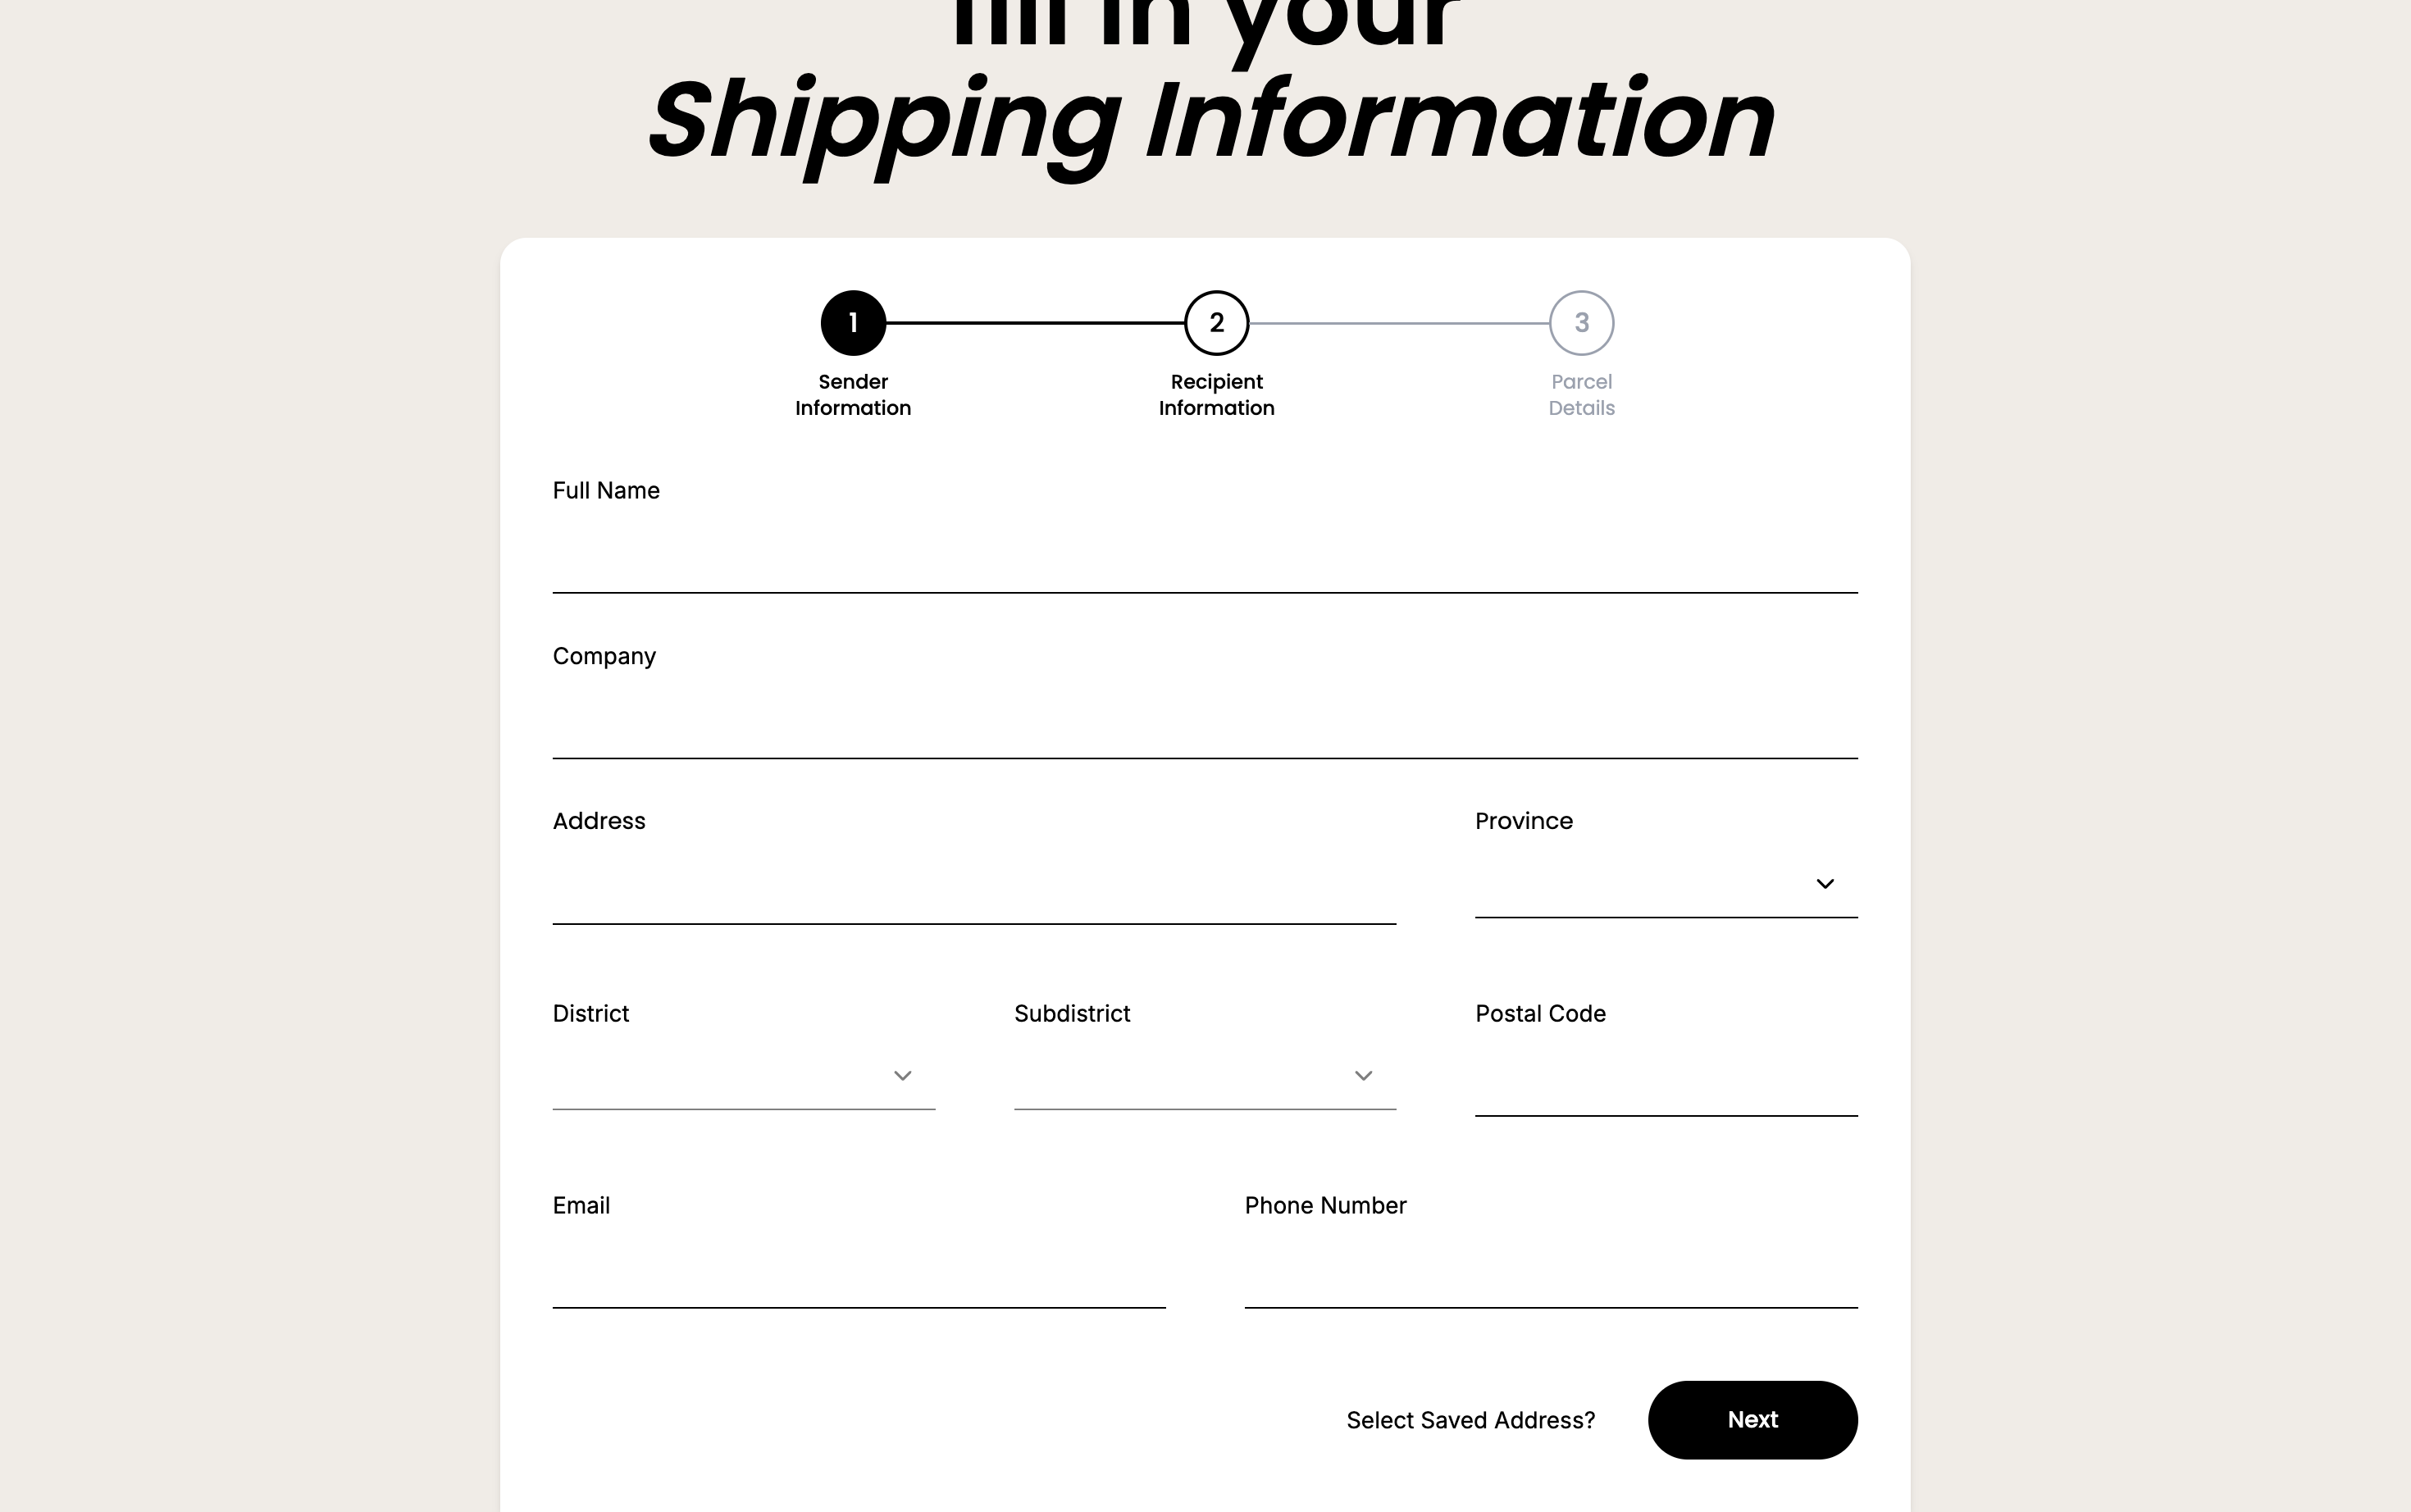
\includegraphics[width=0.8\textwidth]{fillrecipientaddress.png}
    \caption{หน้ากรอกข้อมูลผู้รับ}
    \label{fig:ui_user_recipient}
\end{figure}
\end{minipage}

\vspace{1em}
\begin{minipage}{\linewidth}
\noindent \textbf{4. หน้าเพิ่มที่อยู่จัดส่ง} \\
สำหรับให้ \textbf{ผู้ส่งพัสดุ} บันทึกข้อมูลที่อยู่ผู้ส่งหรือผู้รับรายการใหม่เข้าสู่ระบบ เพื่อความสะดวกรวดเร็วในการจัดส่งครั้งต่อไป
\begin{figure}[H]
    \centering
    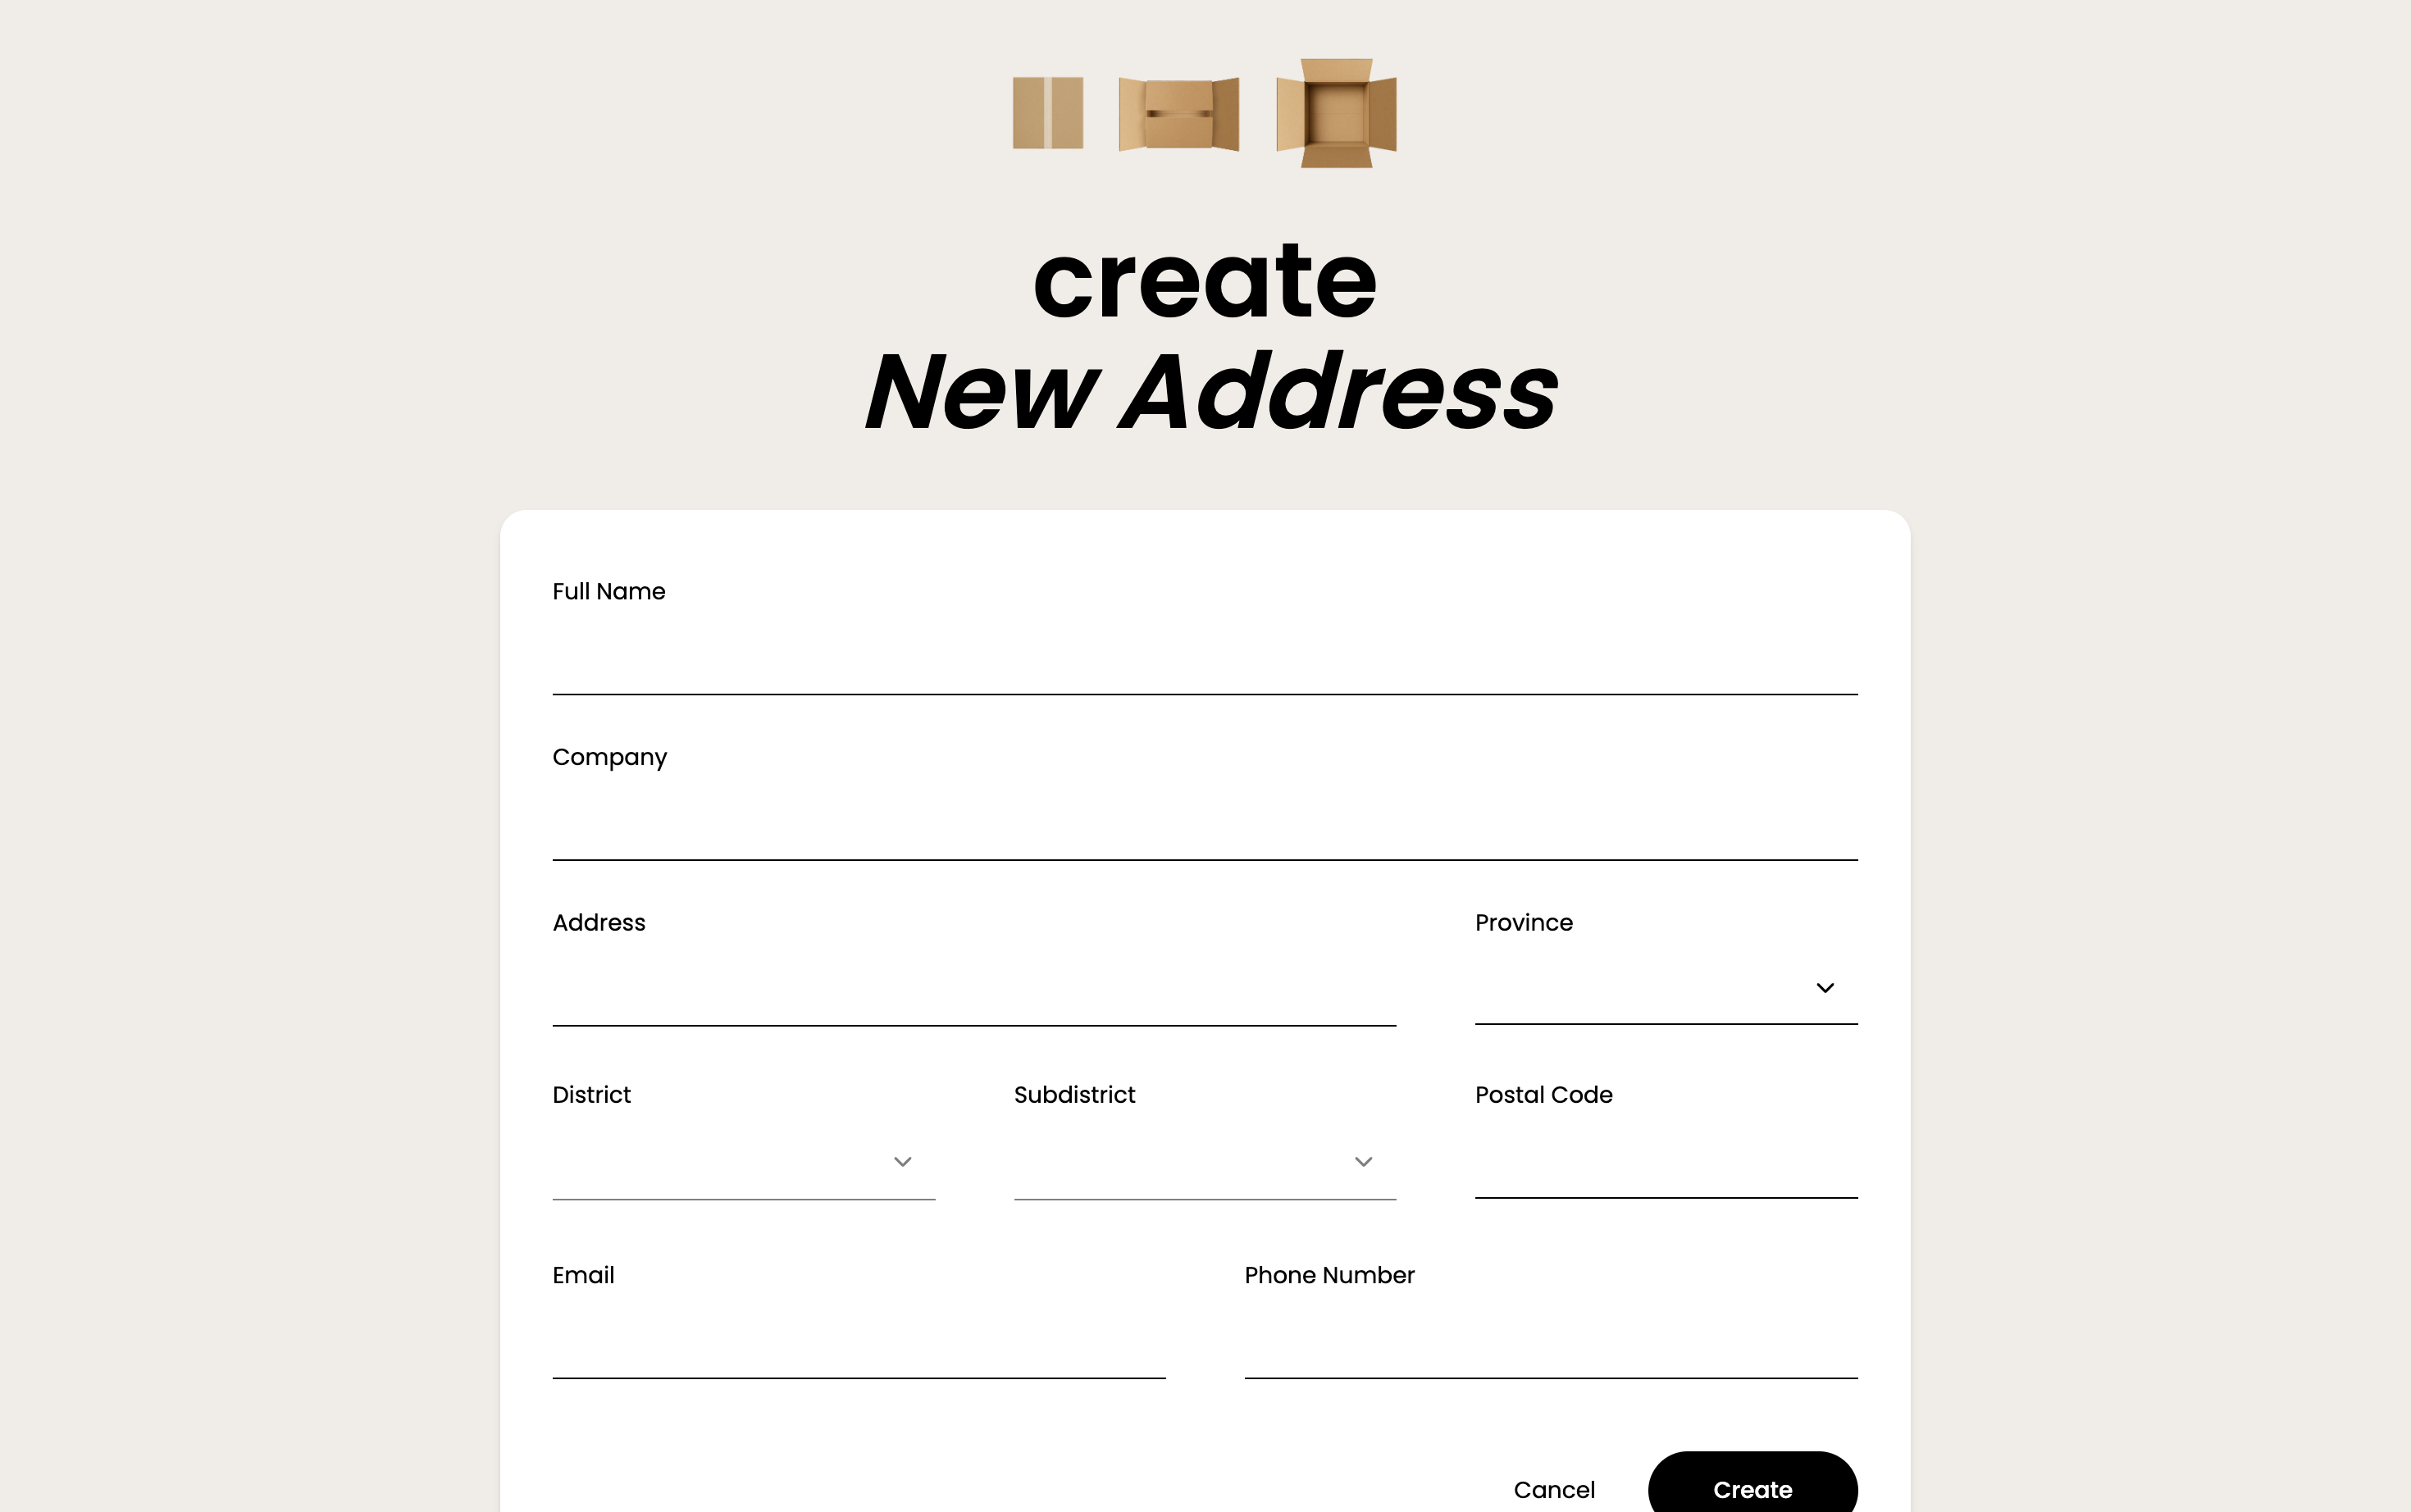
\includegraphics[width=0.8\textwidth]{addsavedaddress.png}
    \caption{หน้าเพิ่มที่อยู่จัดส่ง}
    \label{fig:ui_user_add_address}
\end{figure}
\end{minipage}

\vspace{1em}
\begin{minipage}{\linewidth}
\noindent \textbf{5. หน้าจัดการที่อยู่จัดส่ง} \\
สำหรับให้ \textbf{ผู้ส่งพัสดุ} เรียกดู เลือกใช้งาน หรือแก้ไขข้อมูลที่อยู่ที่เคยถูกบันทึกไว้ในระบบ
\begin{figure}[H]
    \centering
    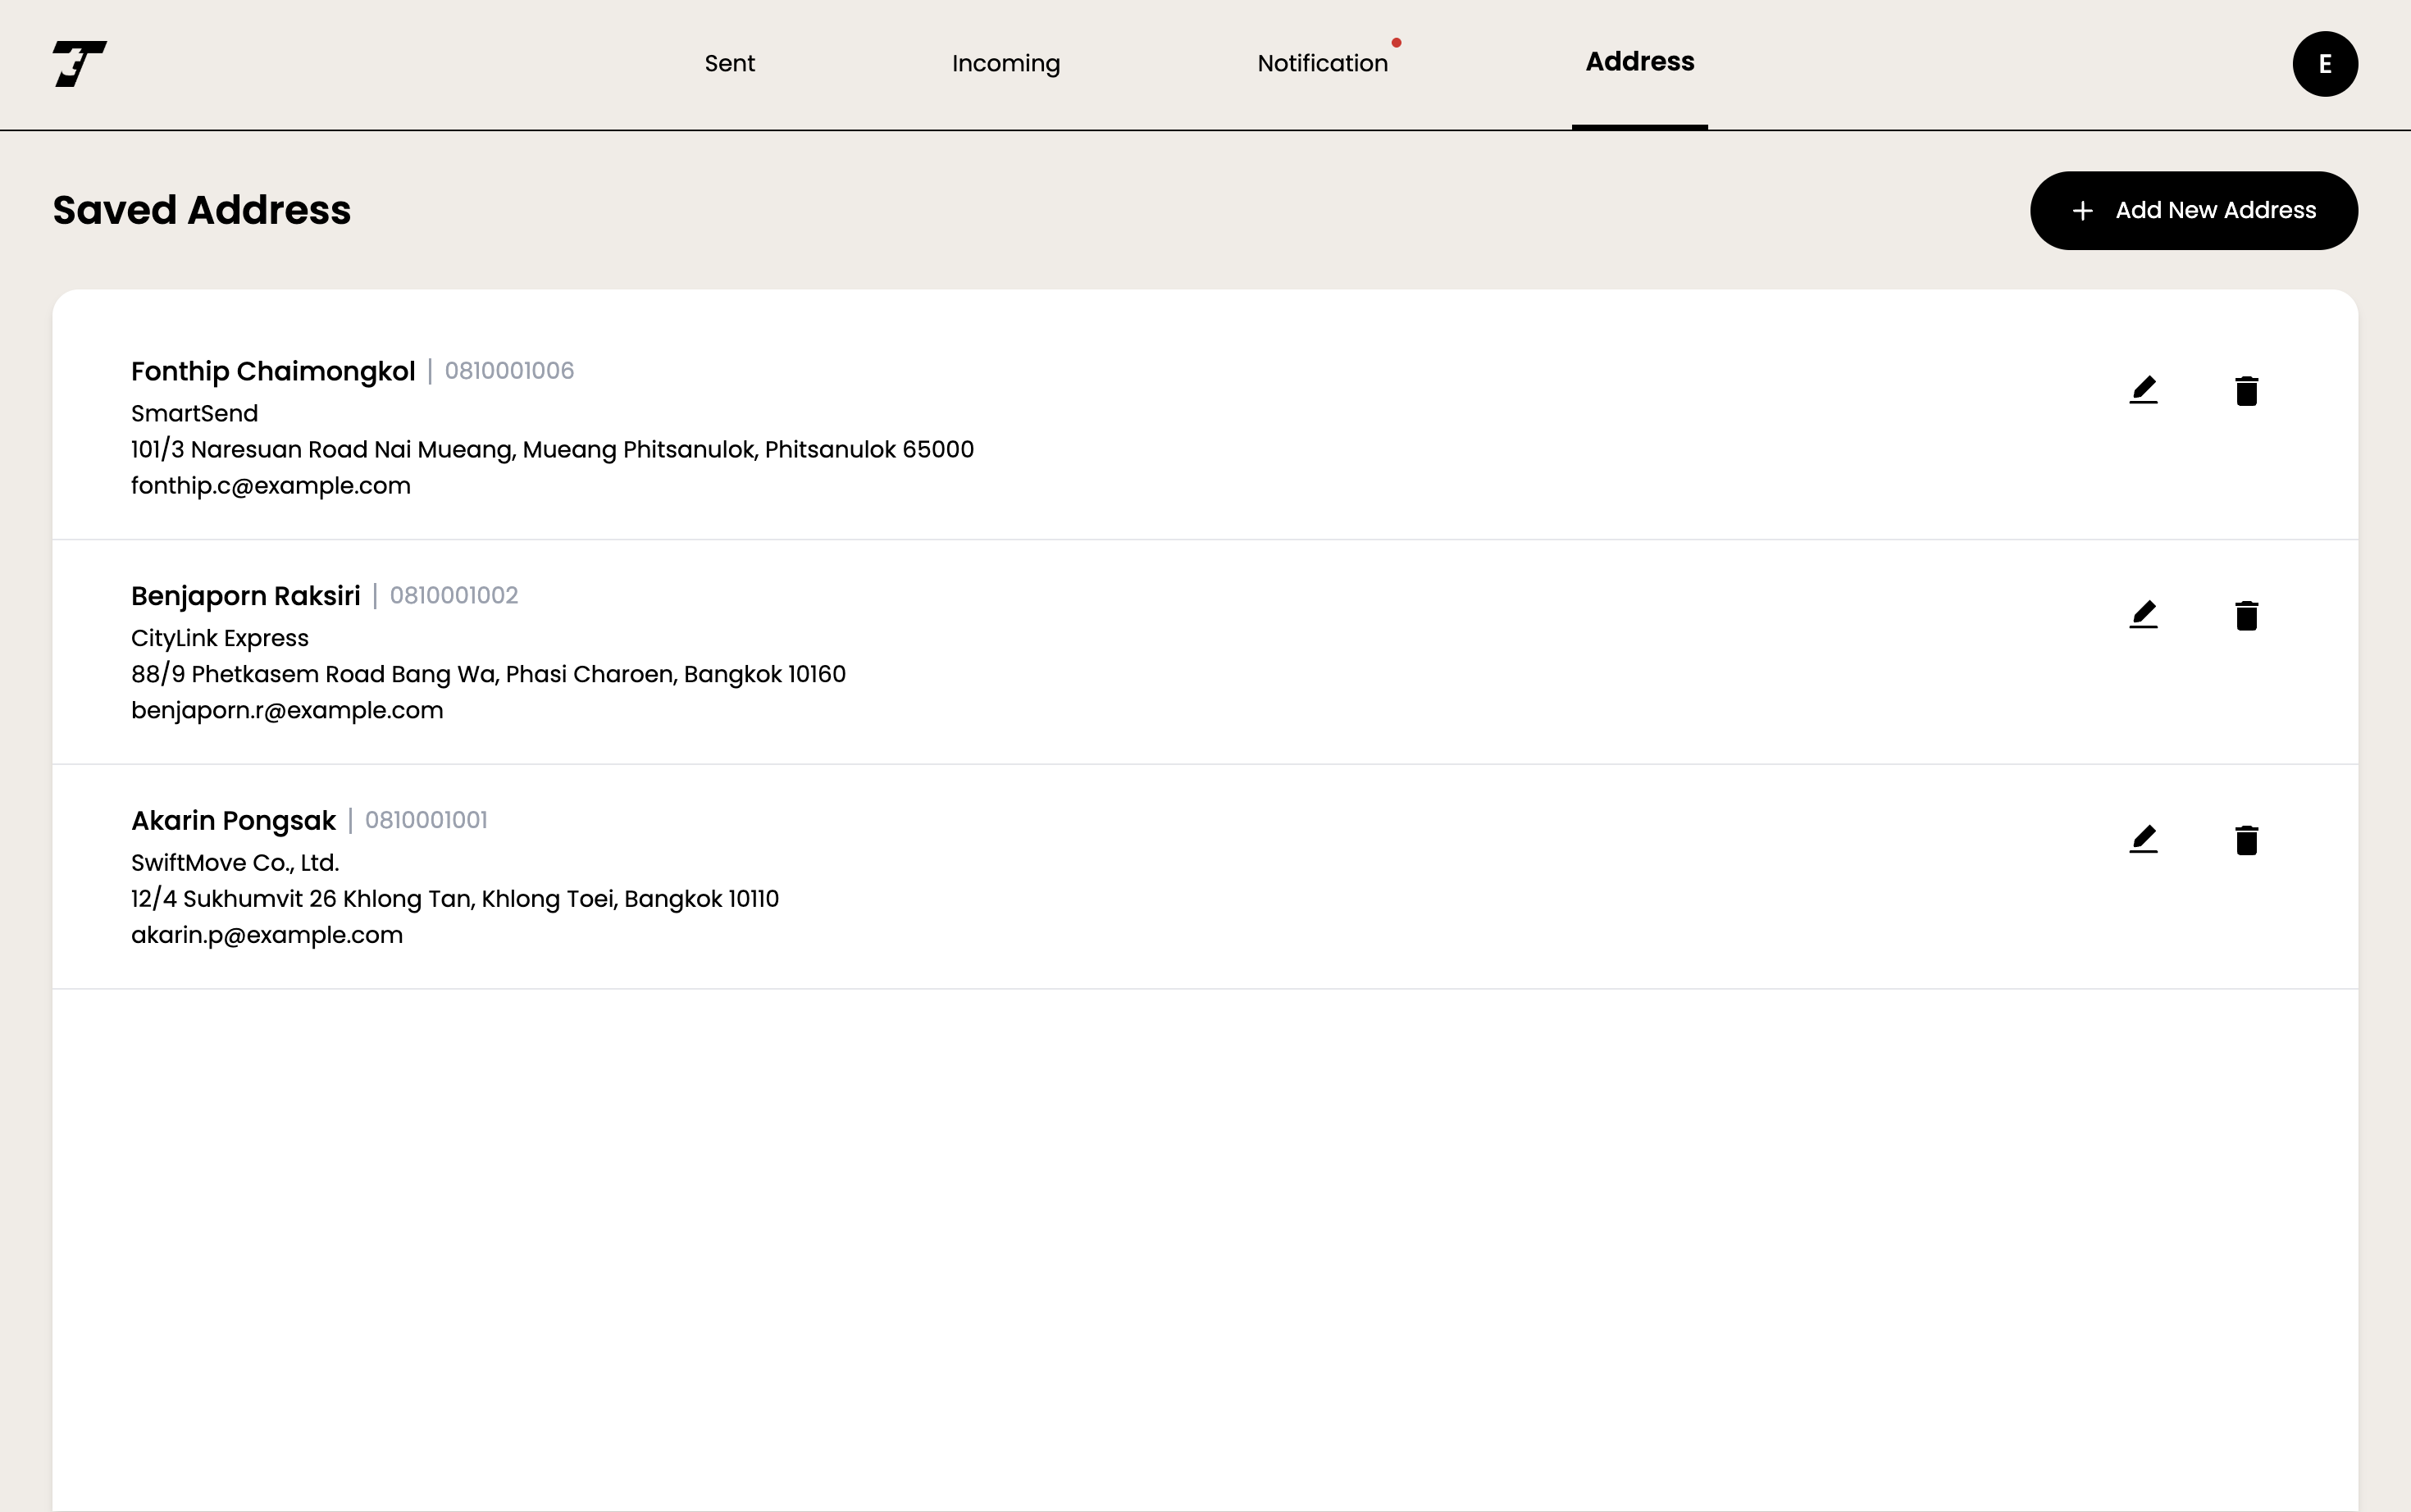
\includegraphics[width=0.8\textwidth]{savedaddress.png}
    \caption{หน้าจัดการที่อยู่จัดส่ง}
    \label{fig:ui_user_saved_address}
\end{figure}
\end{minipage}

\vspace{1em}
\begin{minipage}{\linewidth}
\noindent \textbf{6. หน้าตรวจสอบสถานะ} \\
สำหรับให้ \textbf{ผู้ใช้งานทั่วไปและผู้รับพัสดุ} สามารถกรอกหมายเลขติดตามพัสดุ เพื่อค้นหาสถานะการจัดส่ง
\begin{figure}[H]
    \centering
    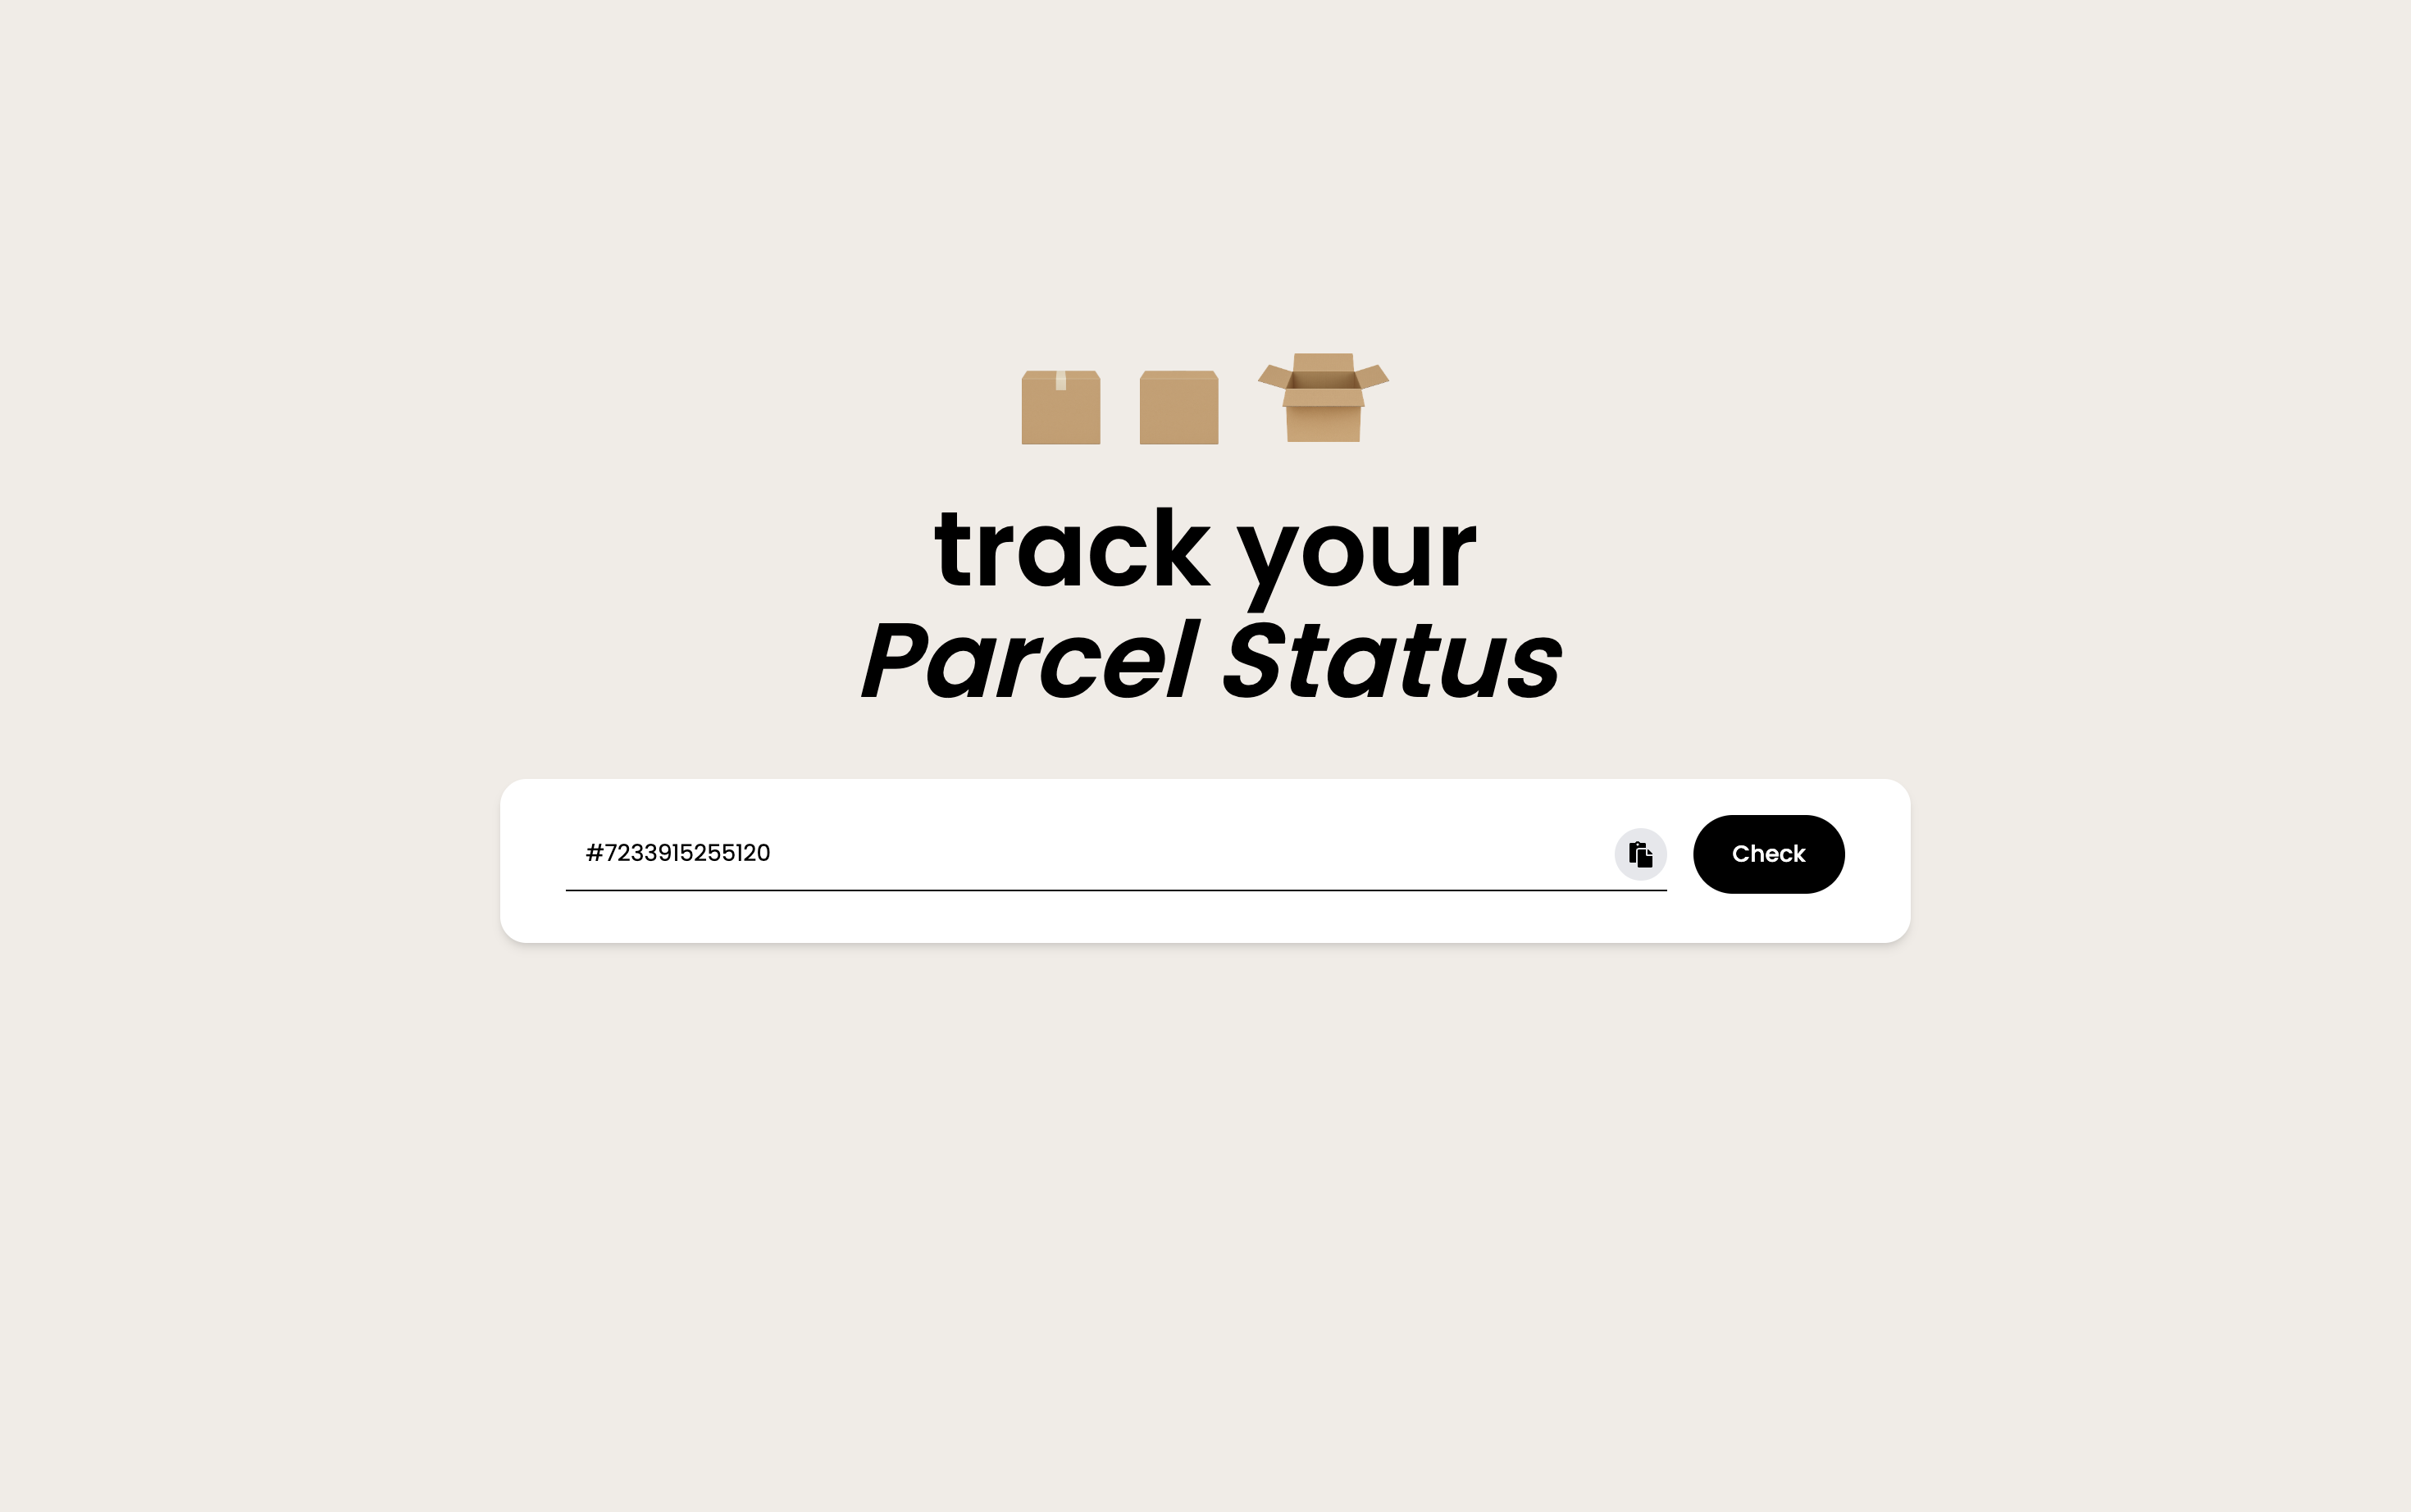
\includegraphics[width=0.8\textwidth]{checktracknum.png}
    \caption{หน้าตรวจสอบสถานะพัสดุ}
    \label{fig:ui_user_track}
\end{figure}
\end{minipage}

\vspace{1em}
\begin{minipage}{\linewidth}
\noindent \textbf{7. หน้ากระดานสรุปผลรายการที่กำลังจัดส่ง} \\
สำหรับให้ \textbf{ผู้รับพัสดุ} ดูสถานะและติดตามพัสดุที่กำลังอยู่ในระหว่างการจัดส่งไปยังจุดหมายปลายทาง
\begin{figure}[H]
    \centering
    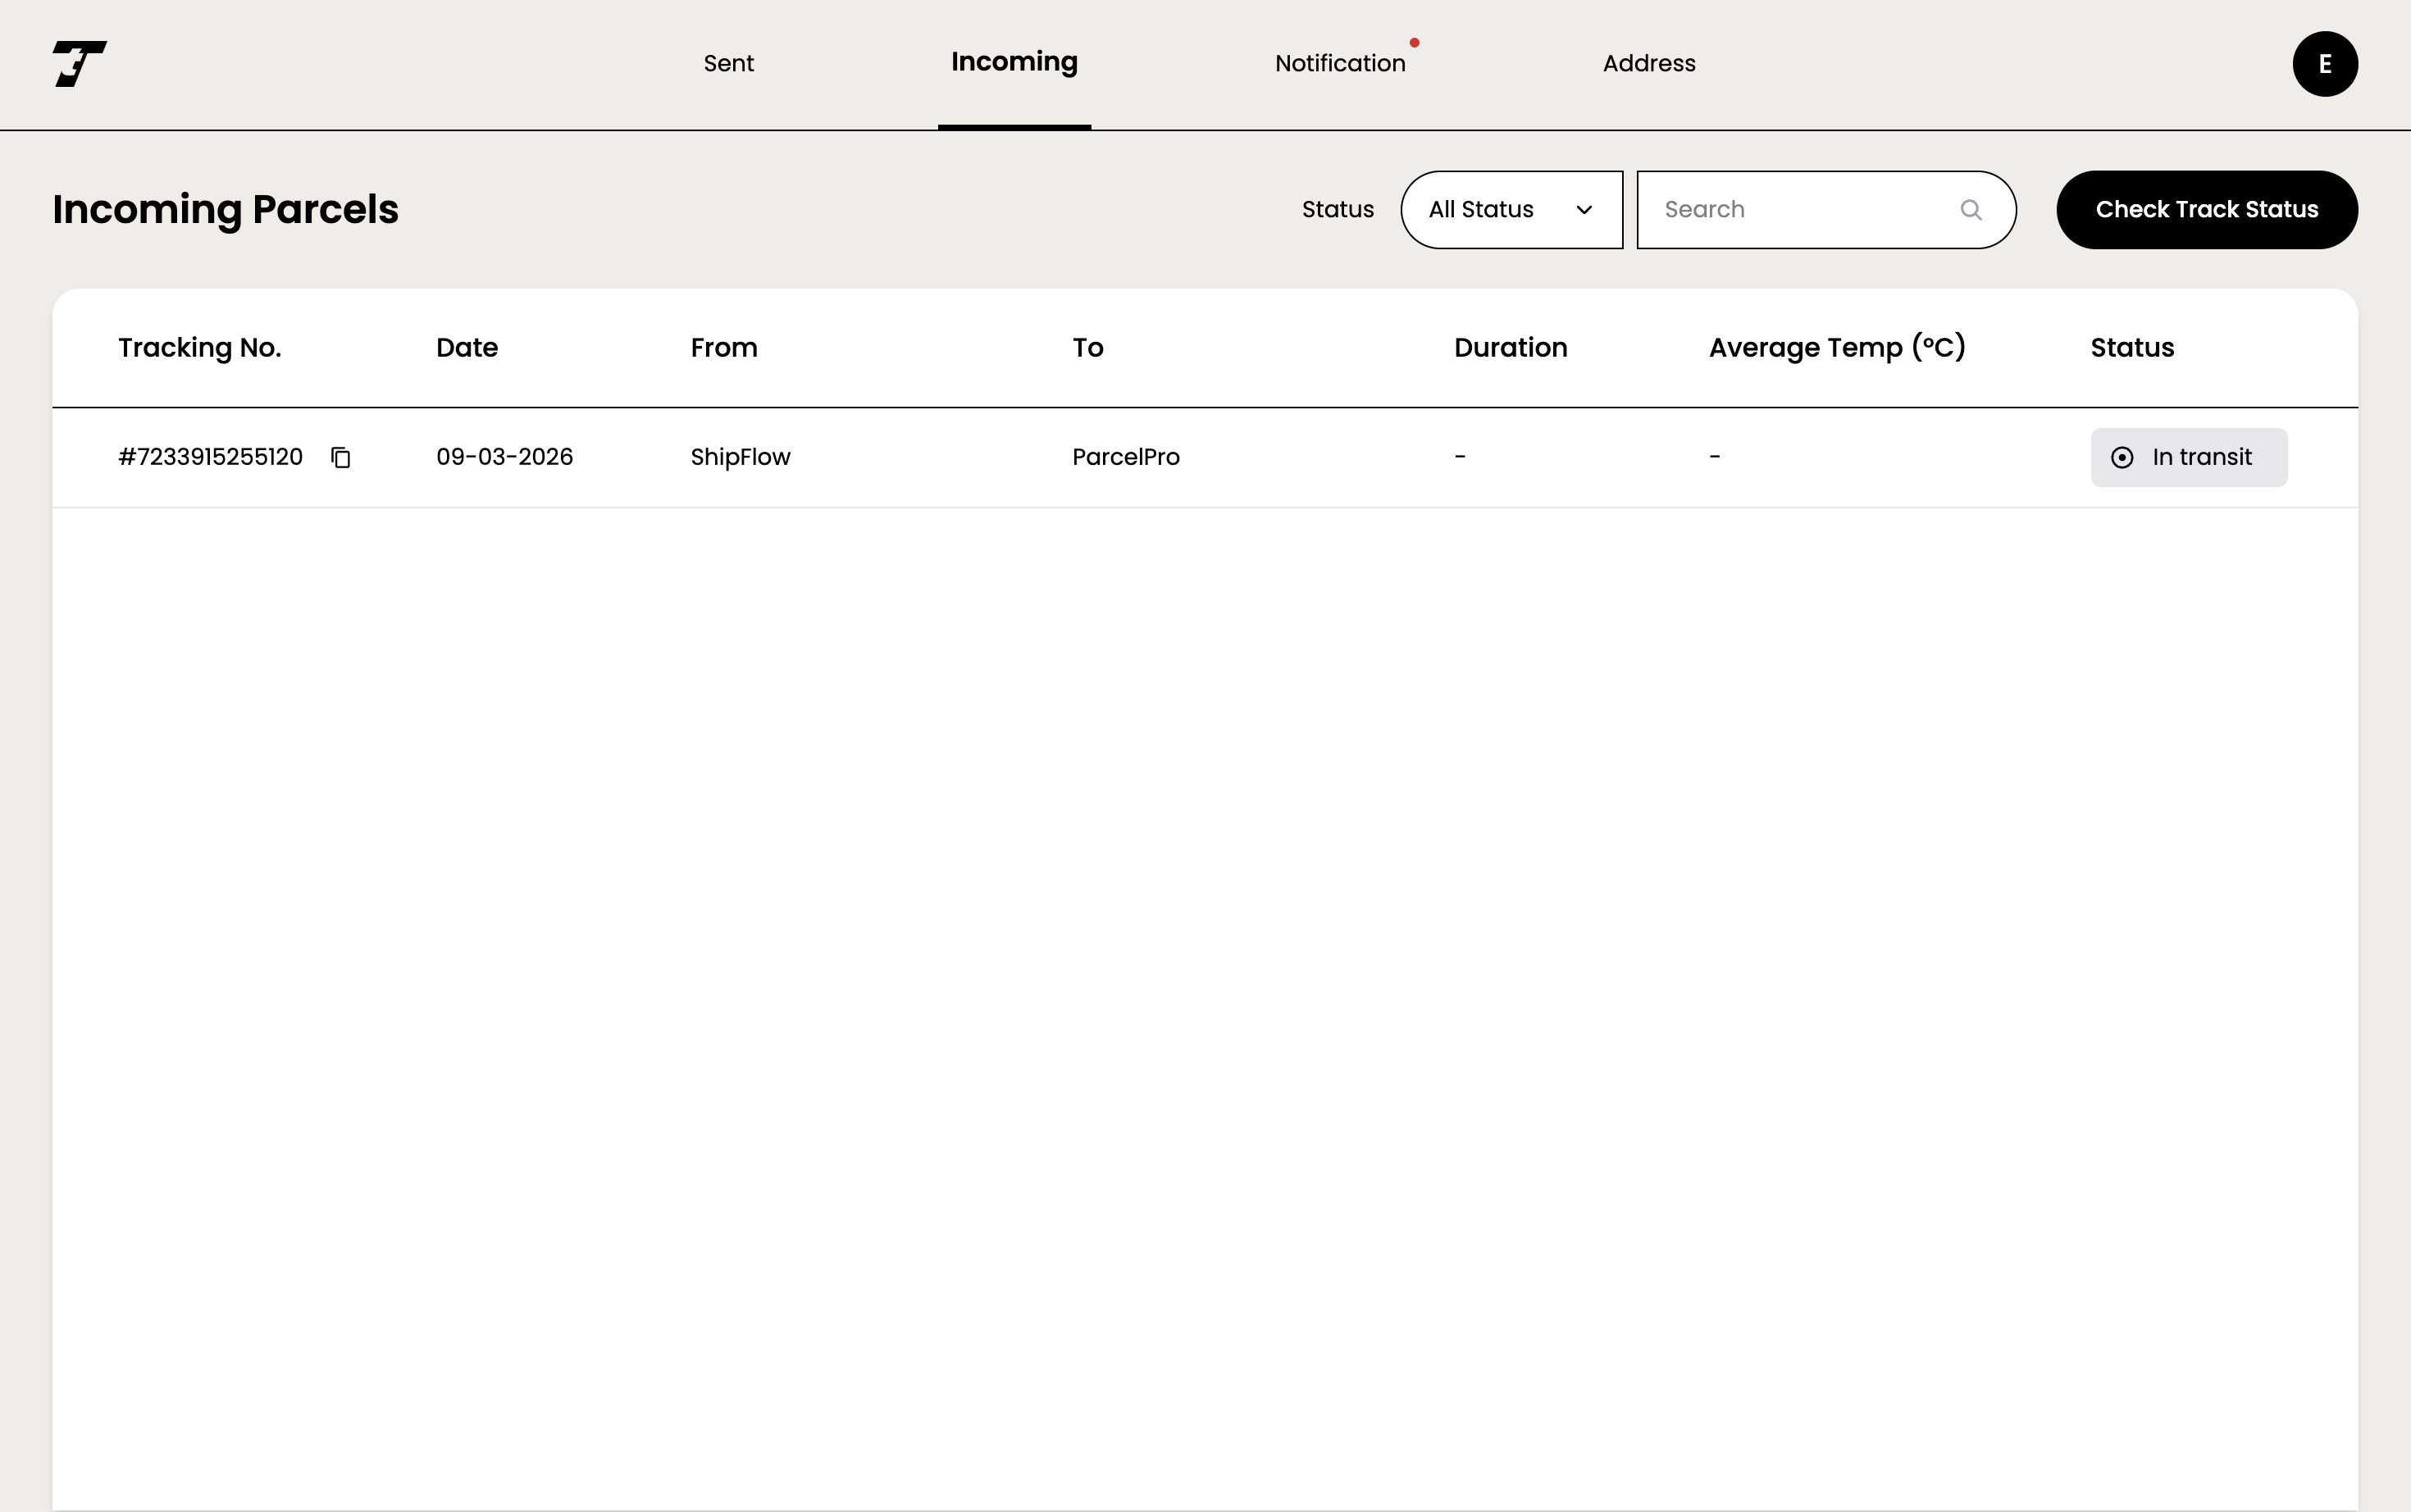
\includegraphics[width=0.8\textwidth]{incoming.png}
    \caption{หน้ากระดานสรุปผลรายการที่กำลังจัดส่ง}
    \label{fig:ui_user_dashboard_incoming}
\end{figure}
\end{minipage}

\vspace{1em}
\begin{minipage}{\linewidth}
\noindent \textbf{8. หน้ากระดานสรุปผลรายการที่ส่งแล้ว} \\
สำหรับดูประวัติและภาพรวมของพัสดุที่ \textbf{ผู้ส่งพัสดุ} ได้ทำการจัดส่งเสร็จสิ้นแล้ว
\begin{figure}[H]
    \centering
    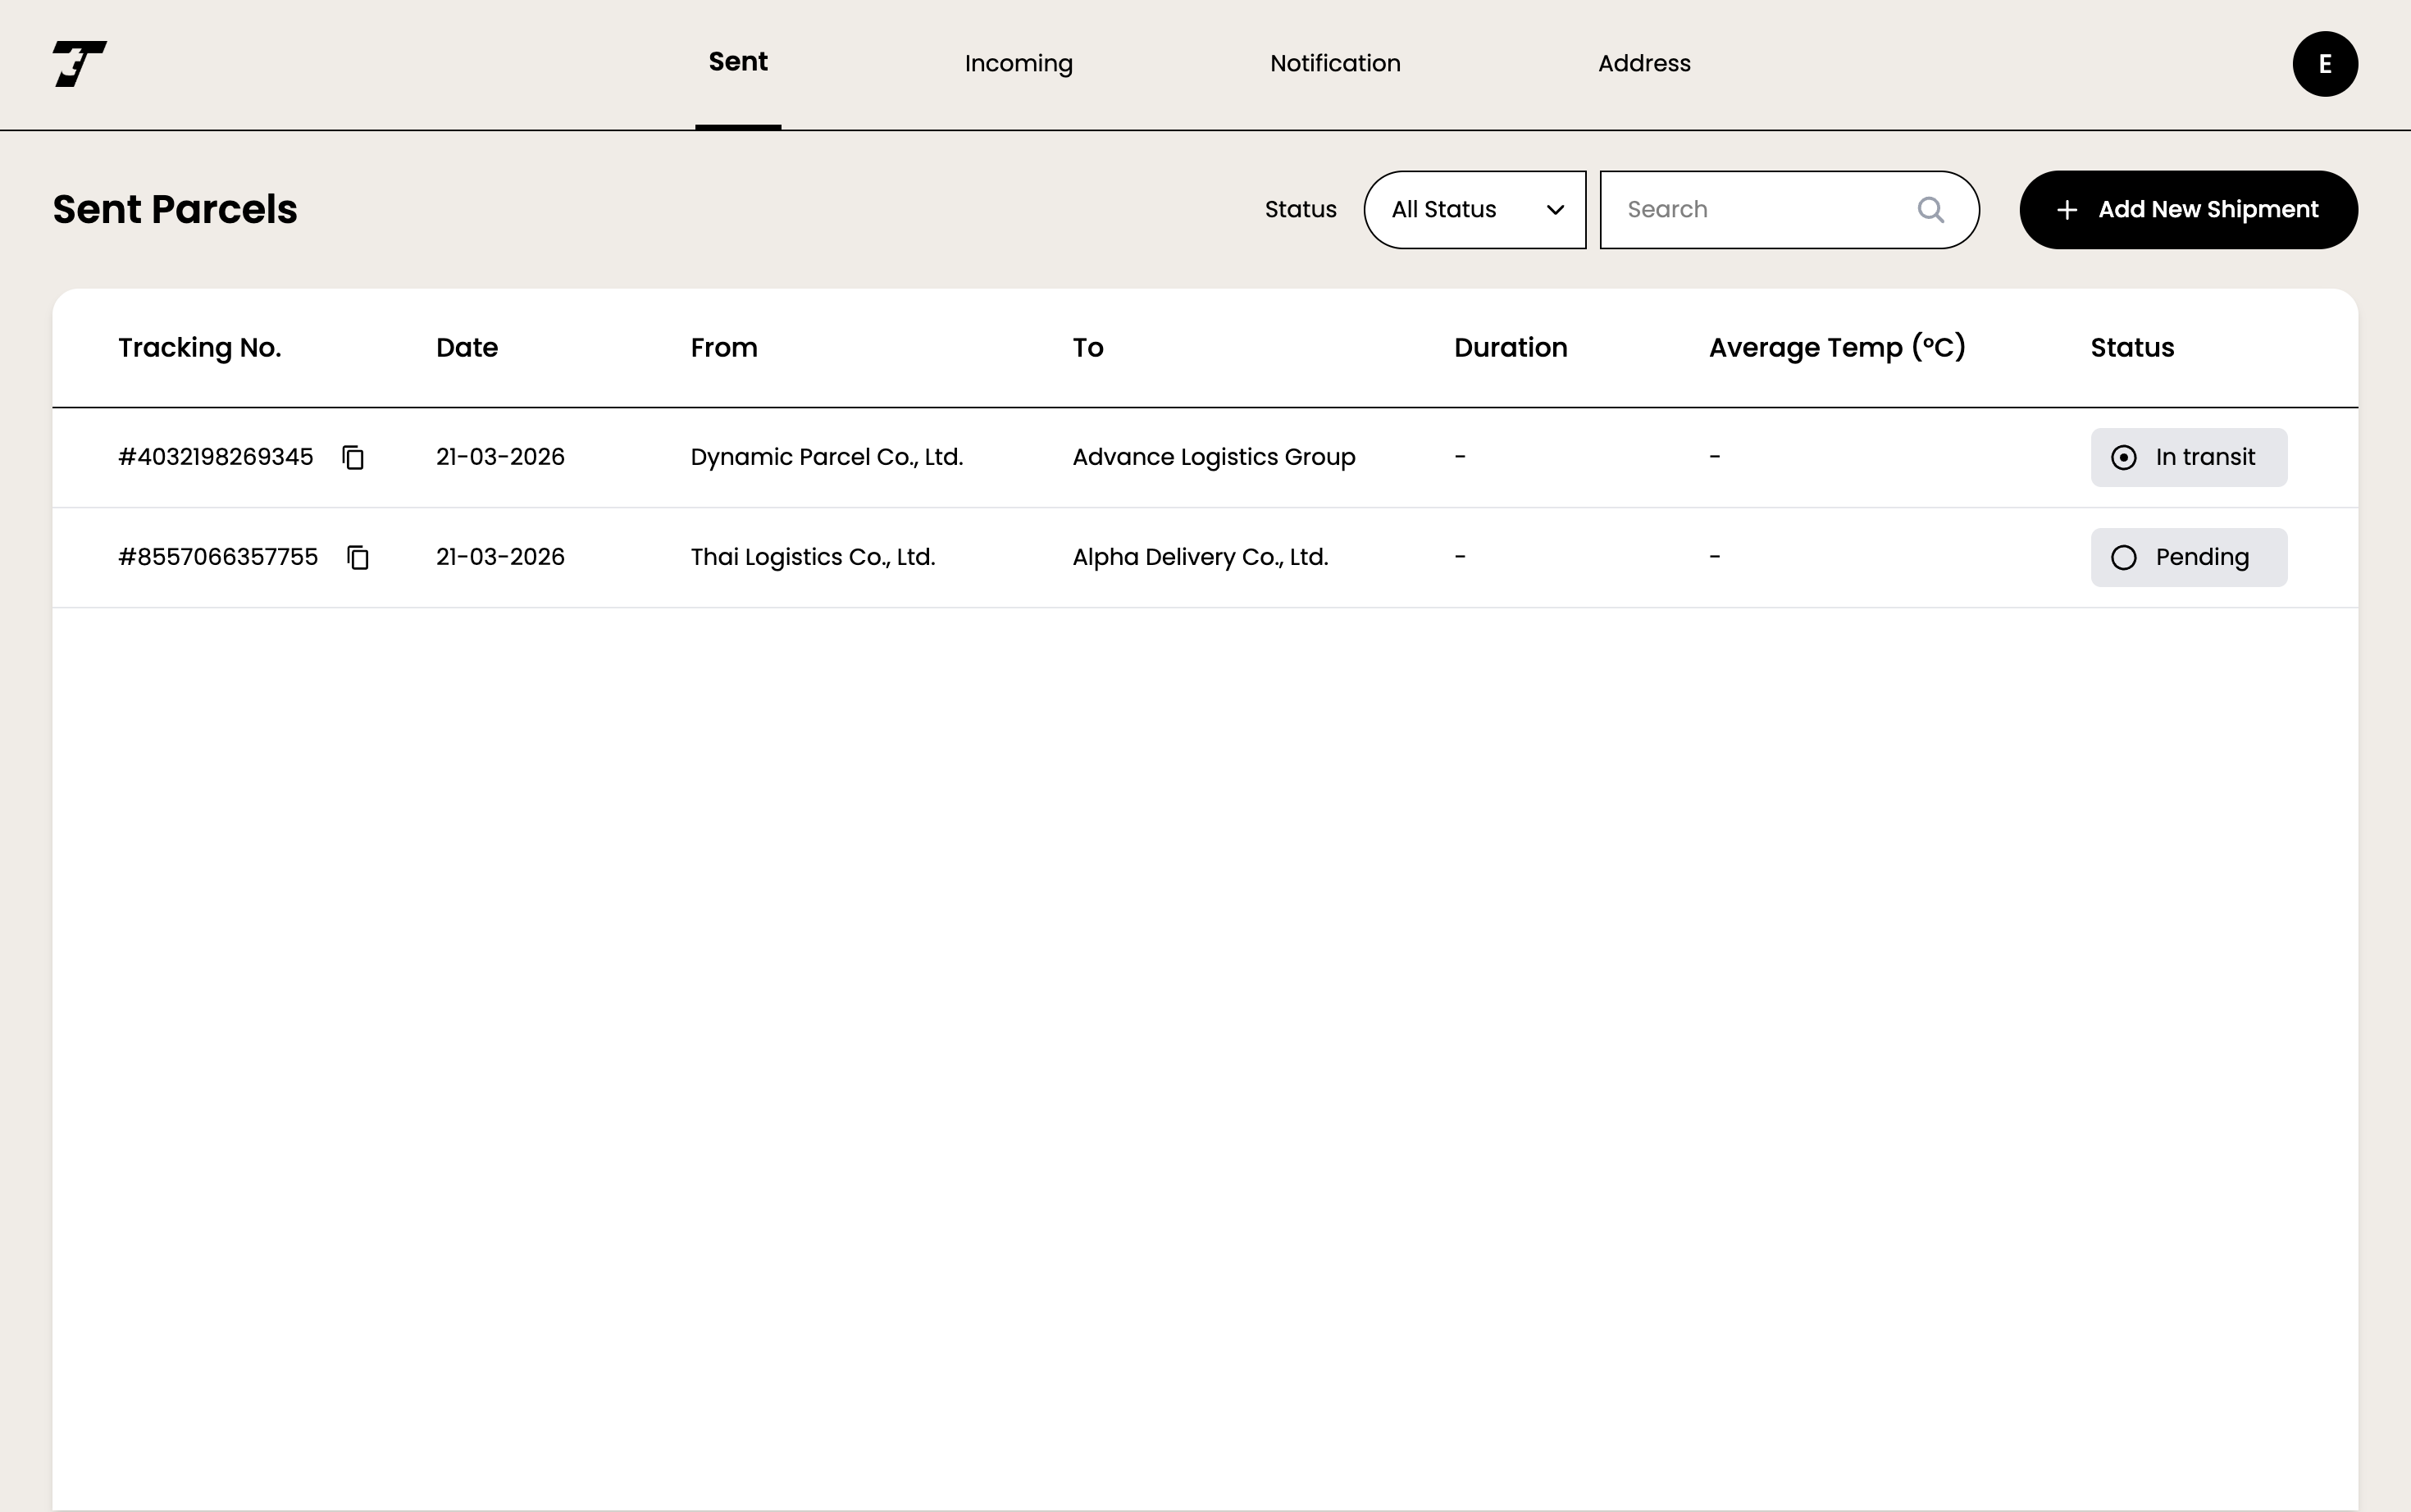
\includegraphics[width=0.8\textwidth]{sent.png}
    \caption{หน้ากระดานสรุปผลรายการที่ส่งแล้ว}
    \label{fig:ui_user_dashboard_sent}
\end{figure}
\end{minipage}

\vspace{1em}
\begin{minipage}{\linewidth}
\noindent \textbf{9. หน้าตรวจสอบอุณหภูมิแบบเรียลไทม์} \\
สำหรับให้ \textbf{ผู้ใช้งานทุกคนที่เกี่ยวข้อง} เฝ้าระวังและดูข้อมูลการเปลี่ยนแปลงของอุณหภูมิพัสดุ ณ เวลาปัจจุบัน (Real-time Monitoring)
\begin{figure}[H]
    \centering
    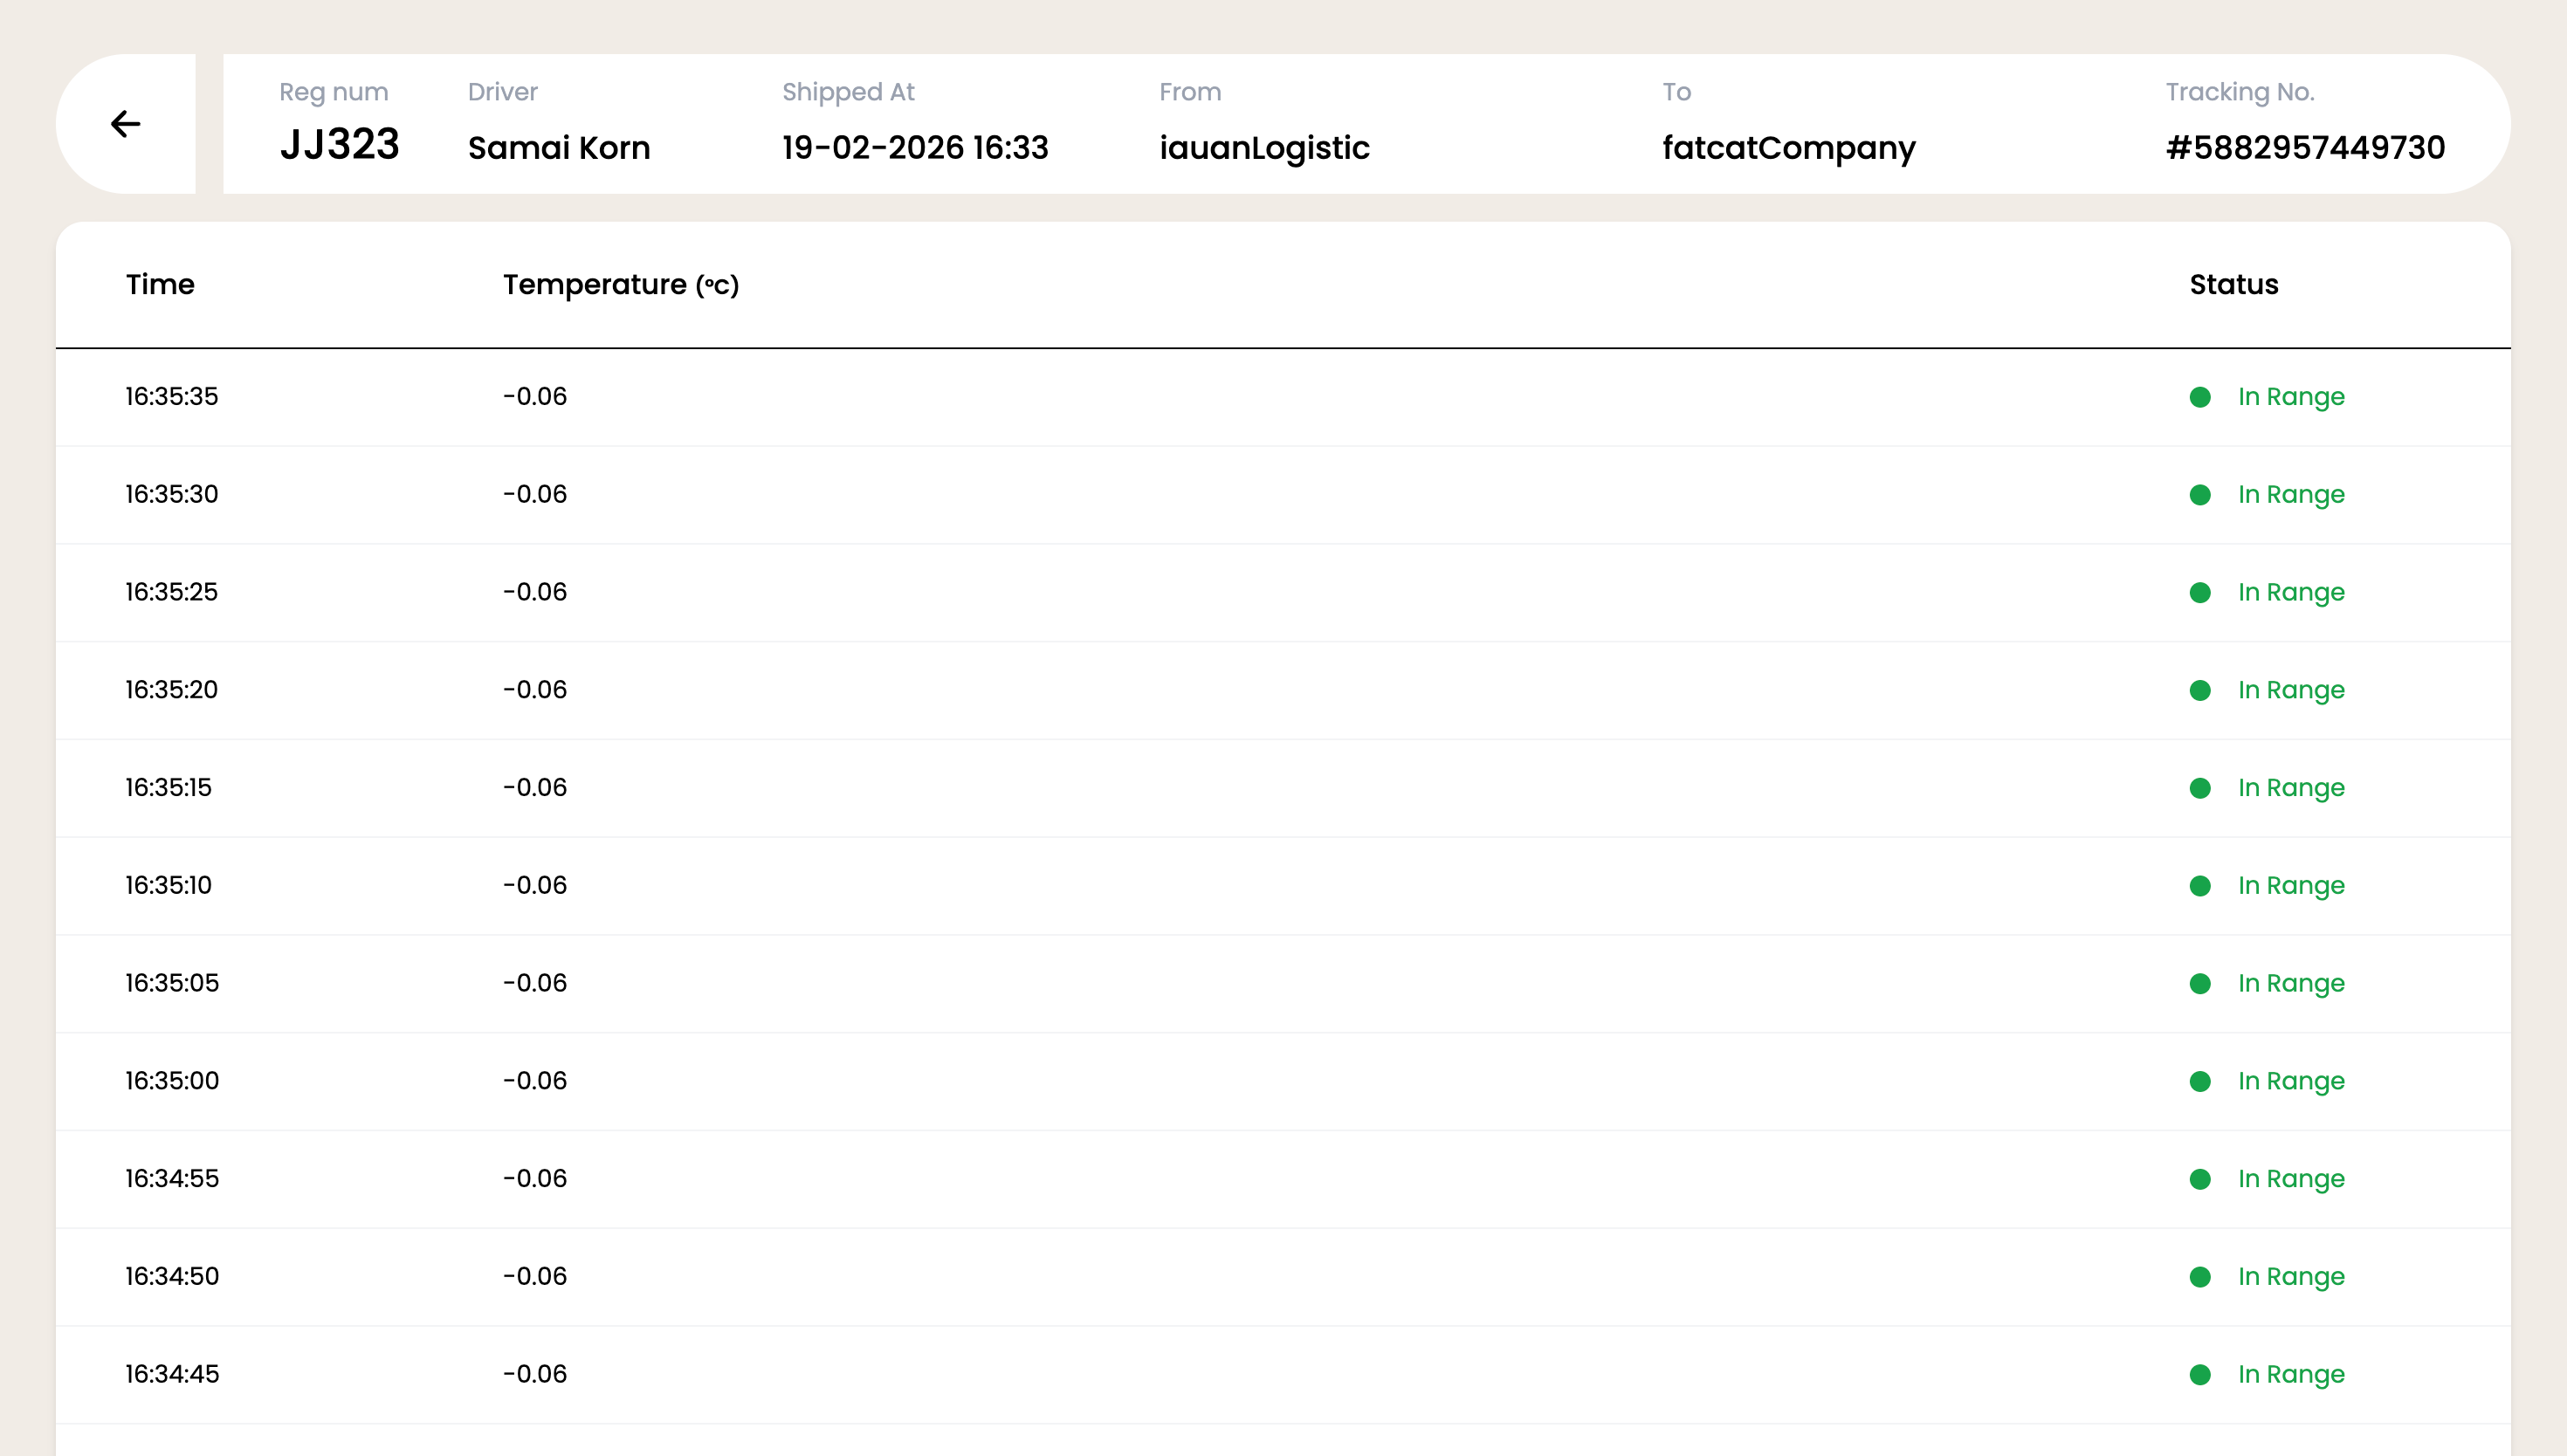
\includegraphics[width=0.8\textwidth]{log.png}
    \caption{หน้าตรวจสอบอุณหภูมิแบบเรียลไทม์}
    \label{fig:ui_user_log}
\end{figure}
\end{minipage}

\vspace{1em}
\begin{minipage}{\linewidth}
\noindent \textbf{10. หน้าการแจ้งเตือน} \\
แสดงการแจ้งเตือนสถานะความคืบหน้าของการจัดส่ง รวมถึงระบบแจ้งเตือนฉุกเฉินหากอุณหภูมิของสินค้าออกนอกเกณฑ์
\begin{figure}[H]
    \centering
    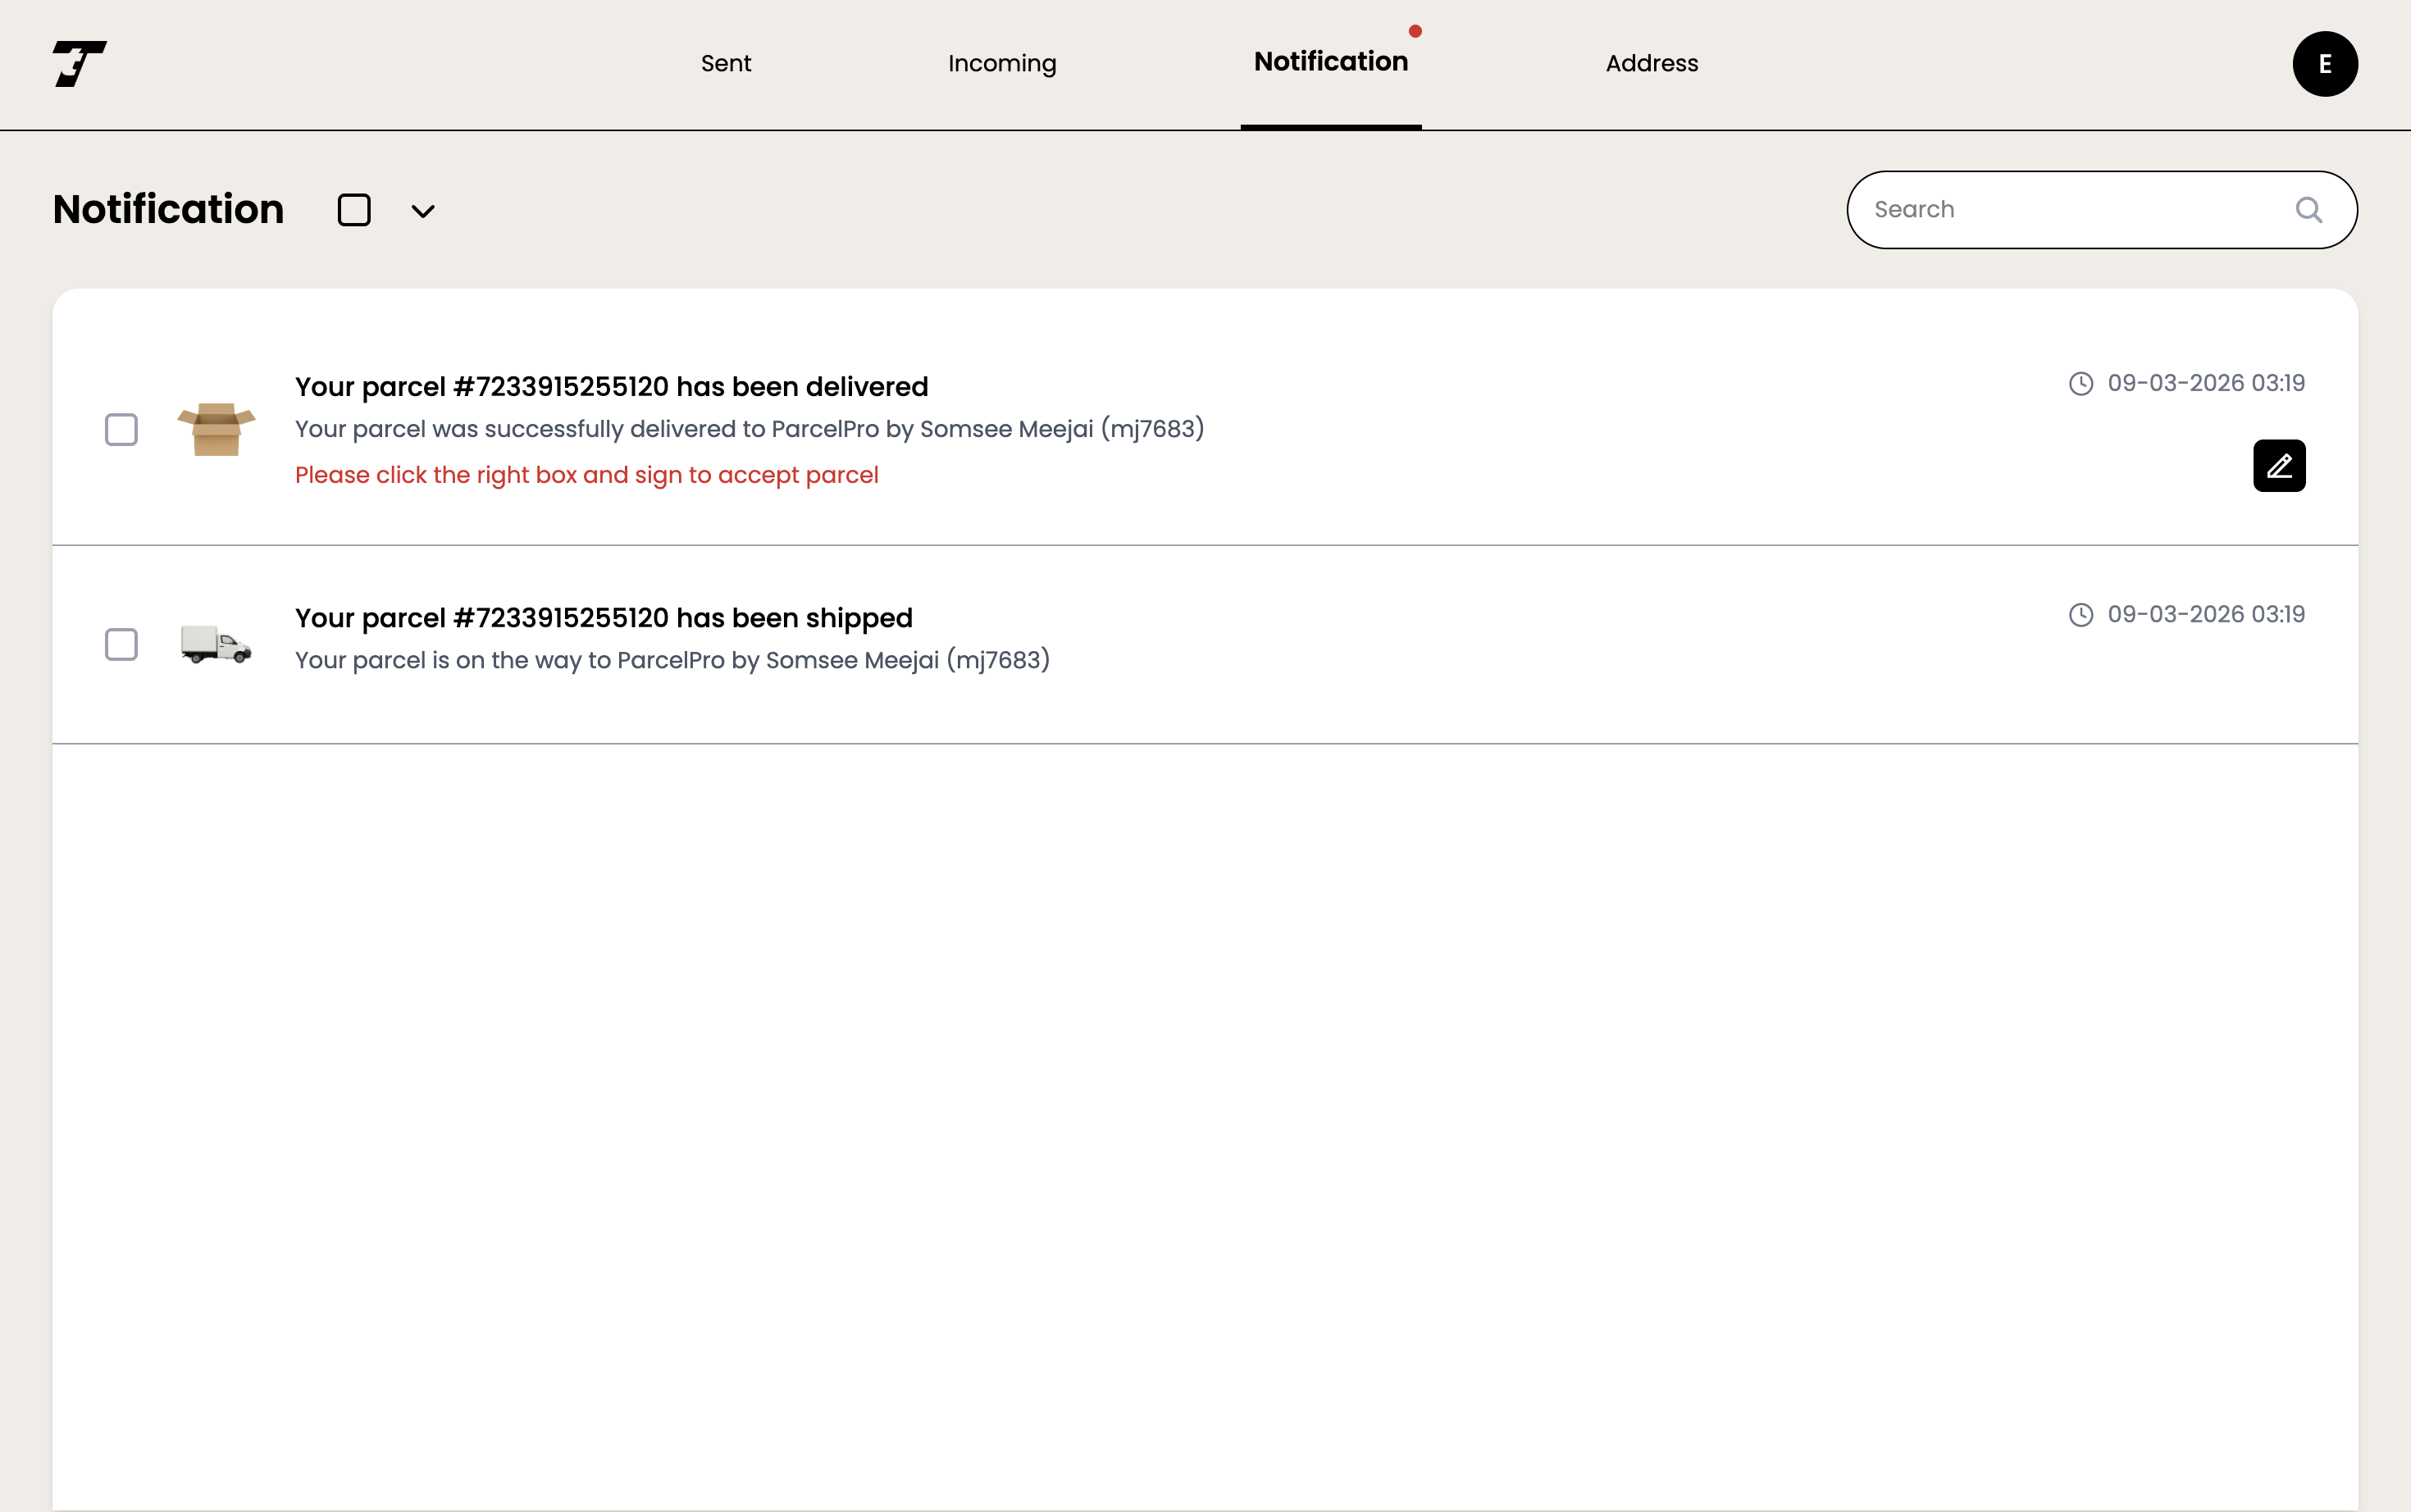
\includegraphics[width=0.8\textwidth]{notification.png}
    \caption{หน้าการแจ้งเตือนสำหรับผู้ใช้งานทั่วไป}
    \label{fig:ui_user_noti}
\end{figure}
\end{minipage}

\vspace{1em}
\begin{minipage}{\linewidth}
\noindent \textbf{11. หน้าลายมือชื่อดิจิทัล} \\
สำหรับให้ \textbf{ผู้รับพัสดุ} ทำการเซ็นชื่ออิเล็กทรอนิกส์ผ่านหน้าจอเพื่อยืนยันการรับสินค้าเมื่อพัสดุถูกส่งถึงปลายทาง
\begin{figure}[H]
    \centering
    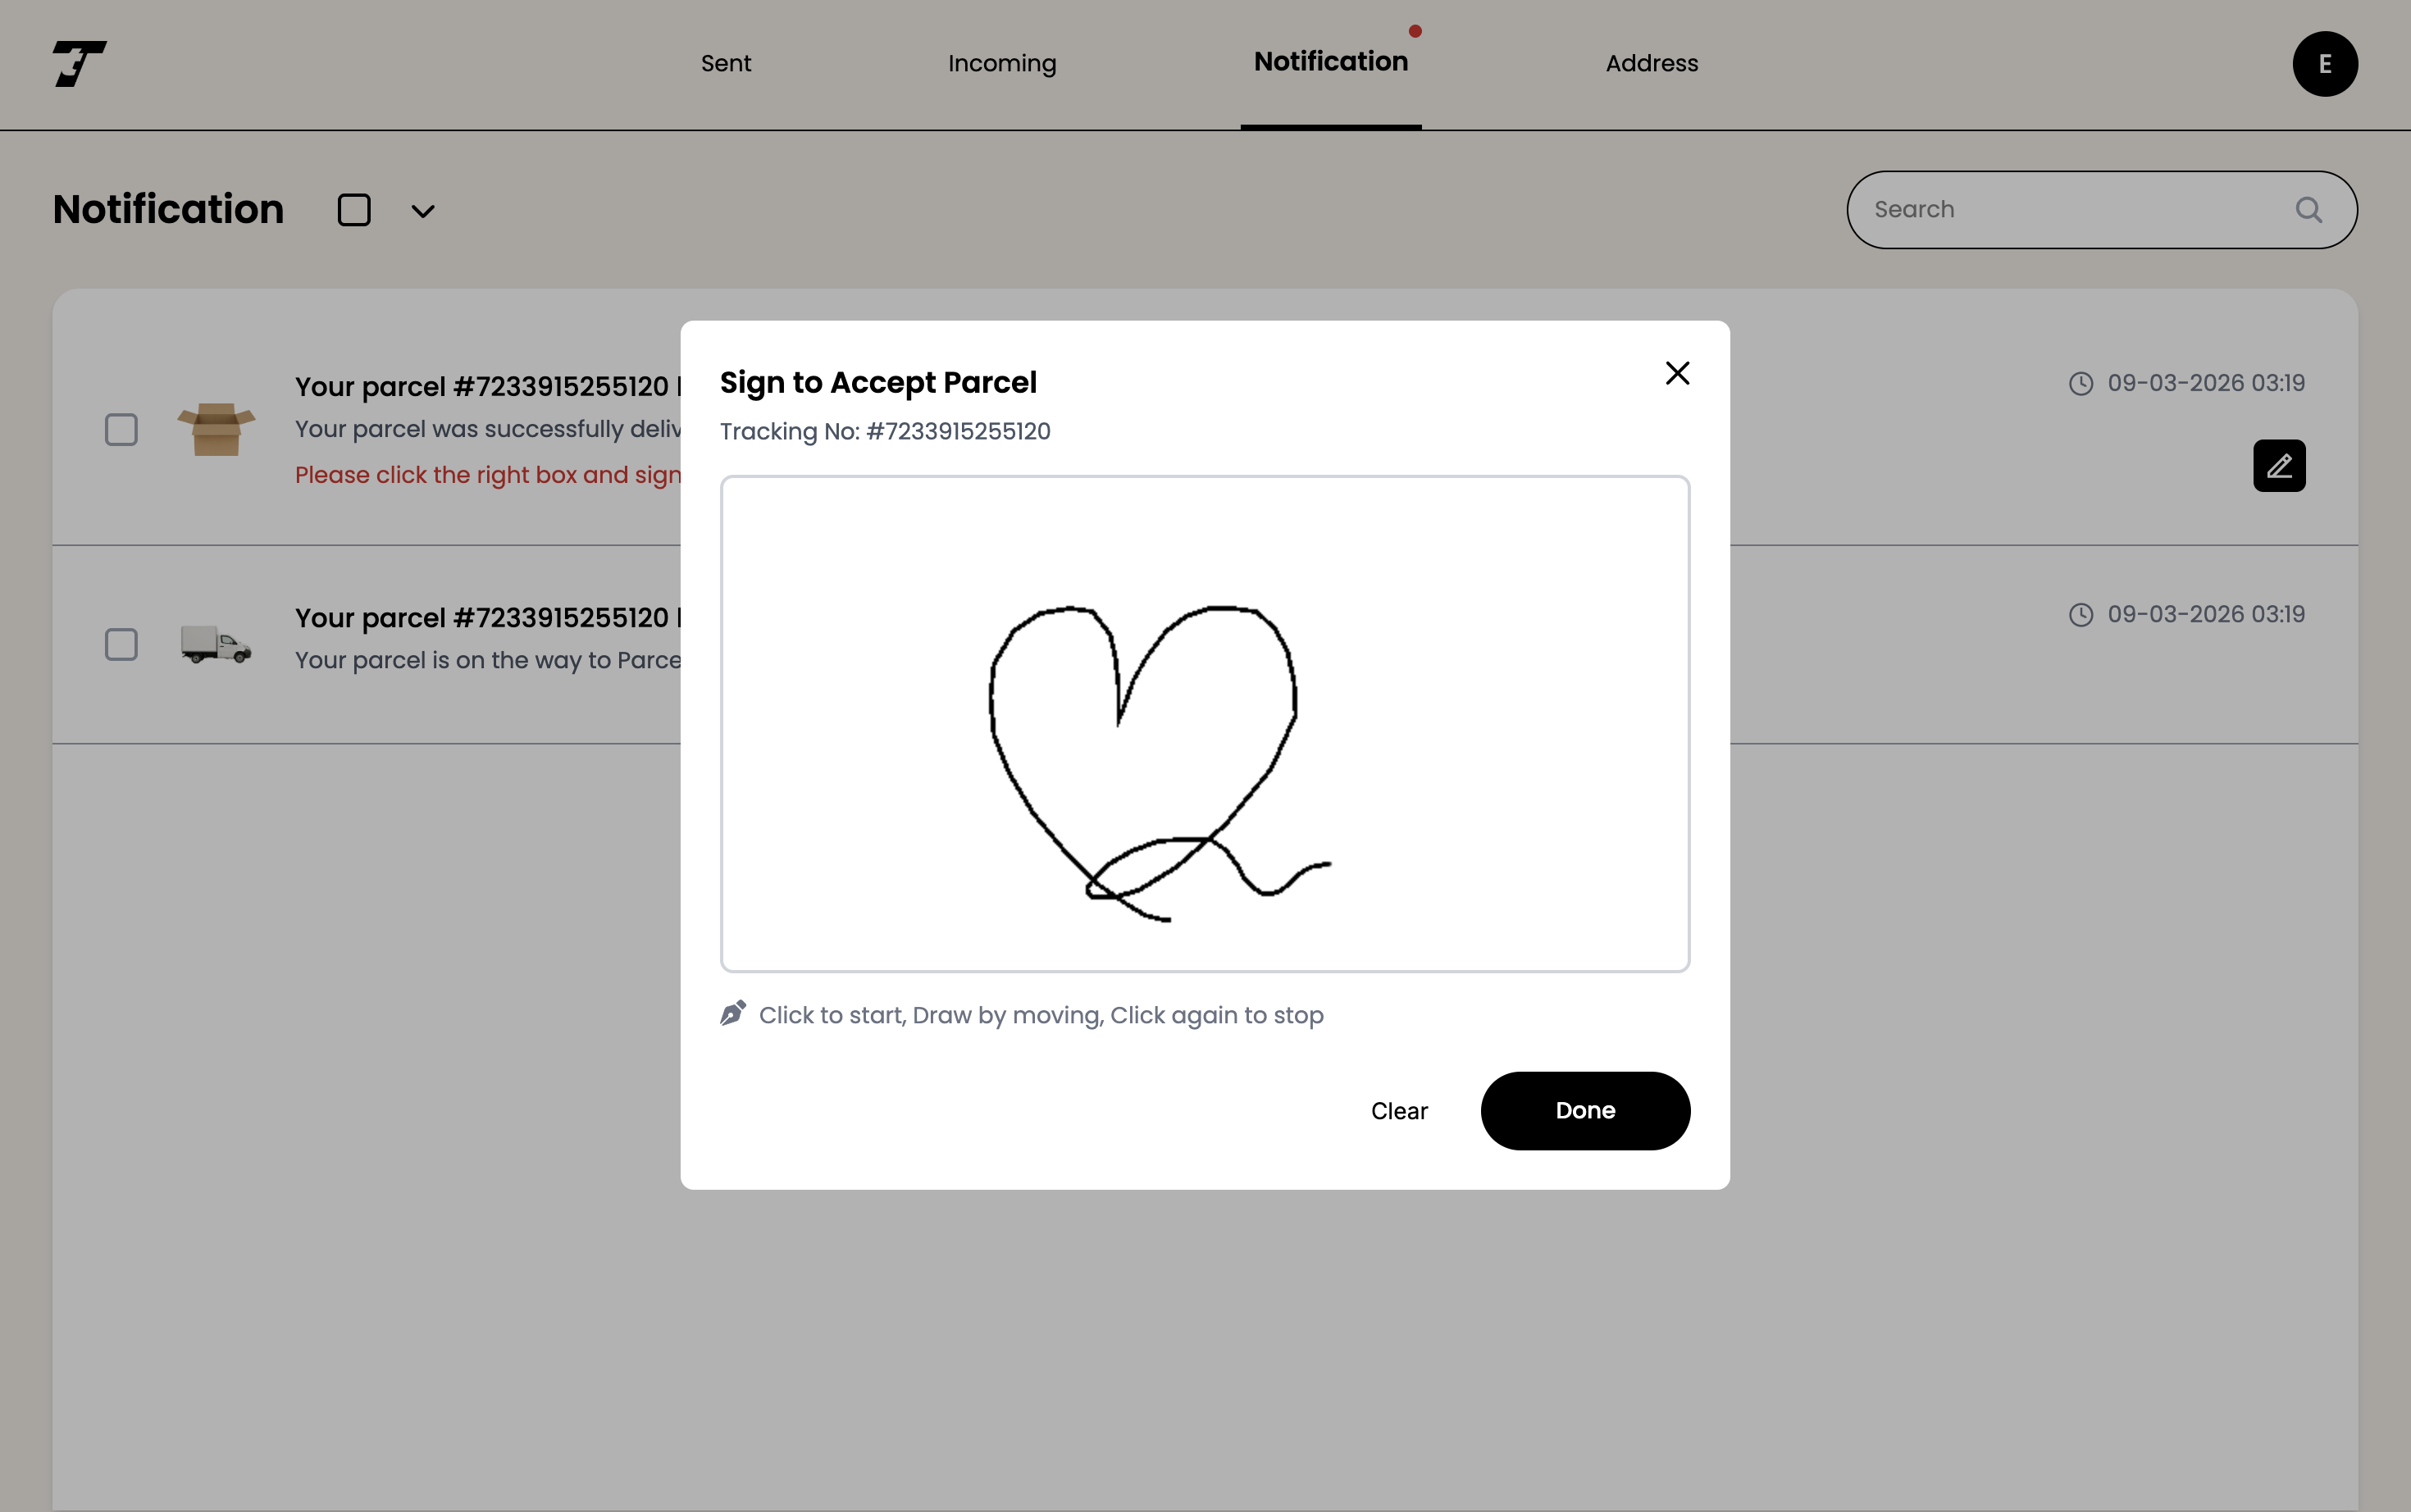
\includegraphics[width=0.8\textwidth]{digitalsignature.png}
    \caption{หน้าลายมือชื่อดิจิทัลสำหรับเซ็นรับพัสดุ}
    \label{fig:ui_user_signature}
\end{figure}
\end{minipage}

\vspace{1em}
\begin{minipage}{\linewidth}
\noindent \textbf{12. หน้าสรุปข้อมูลการขนส่ง} \\
หน้าต่างสรุปข้อมูลแบบเบ็ดเสร็จเมื่อการขนส่งเสร็จสิ้น โดยจะแสดงข้อมูลอุณหภูมิตั้งแต่เริ่มต้นจนถึงปลายทางในรูปแบบกราฟเชิงเวลา พร้อมทั้งแสดงสถานะการยืนยันความถูกต้องของข้อมูล (Verification) ผ่านบล็อกเชน
\begin{figure}[H]
    \centering
    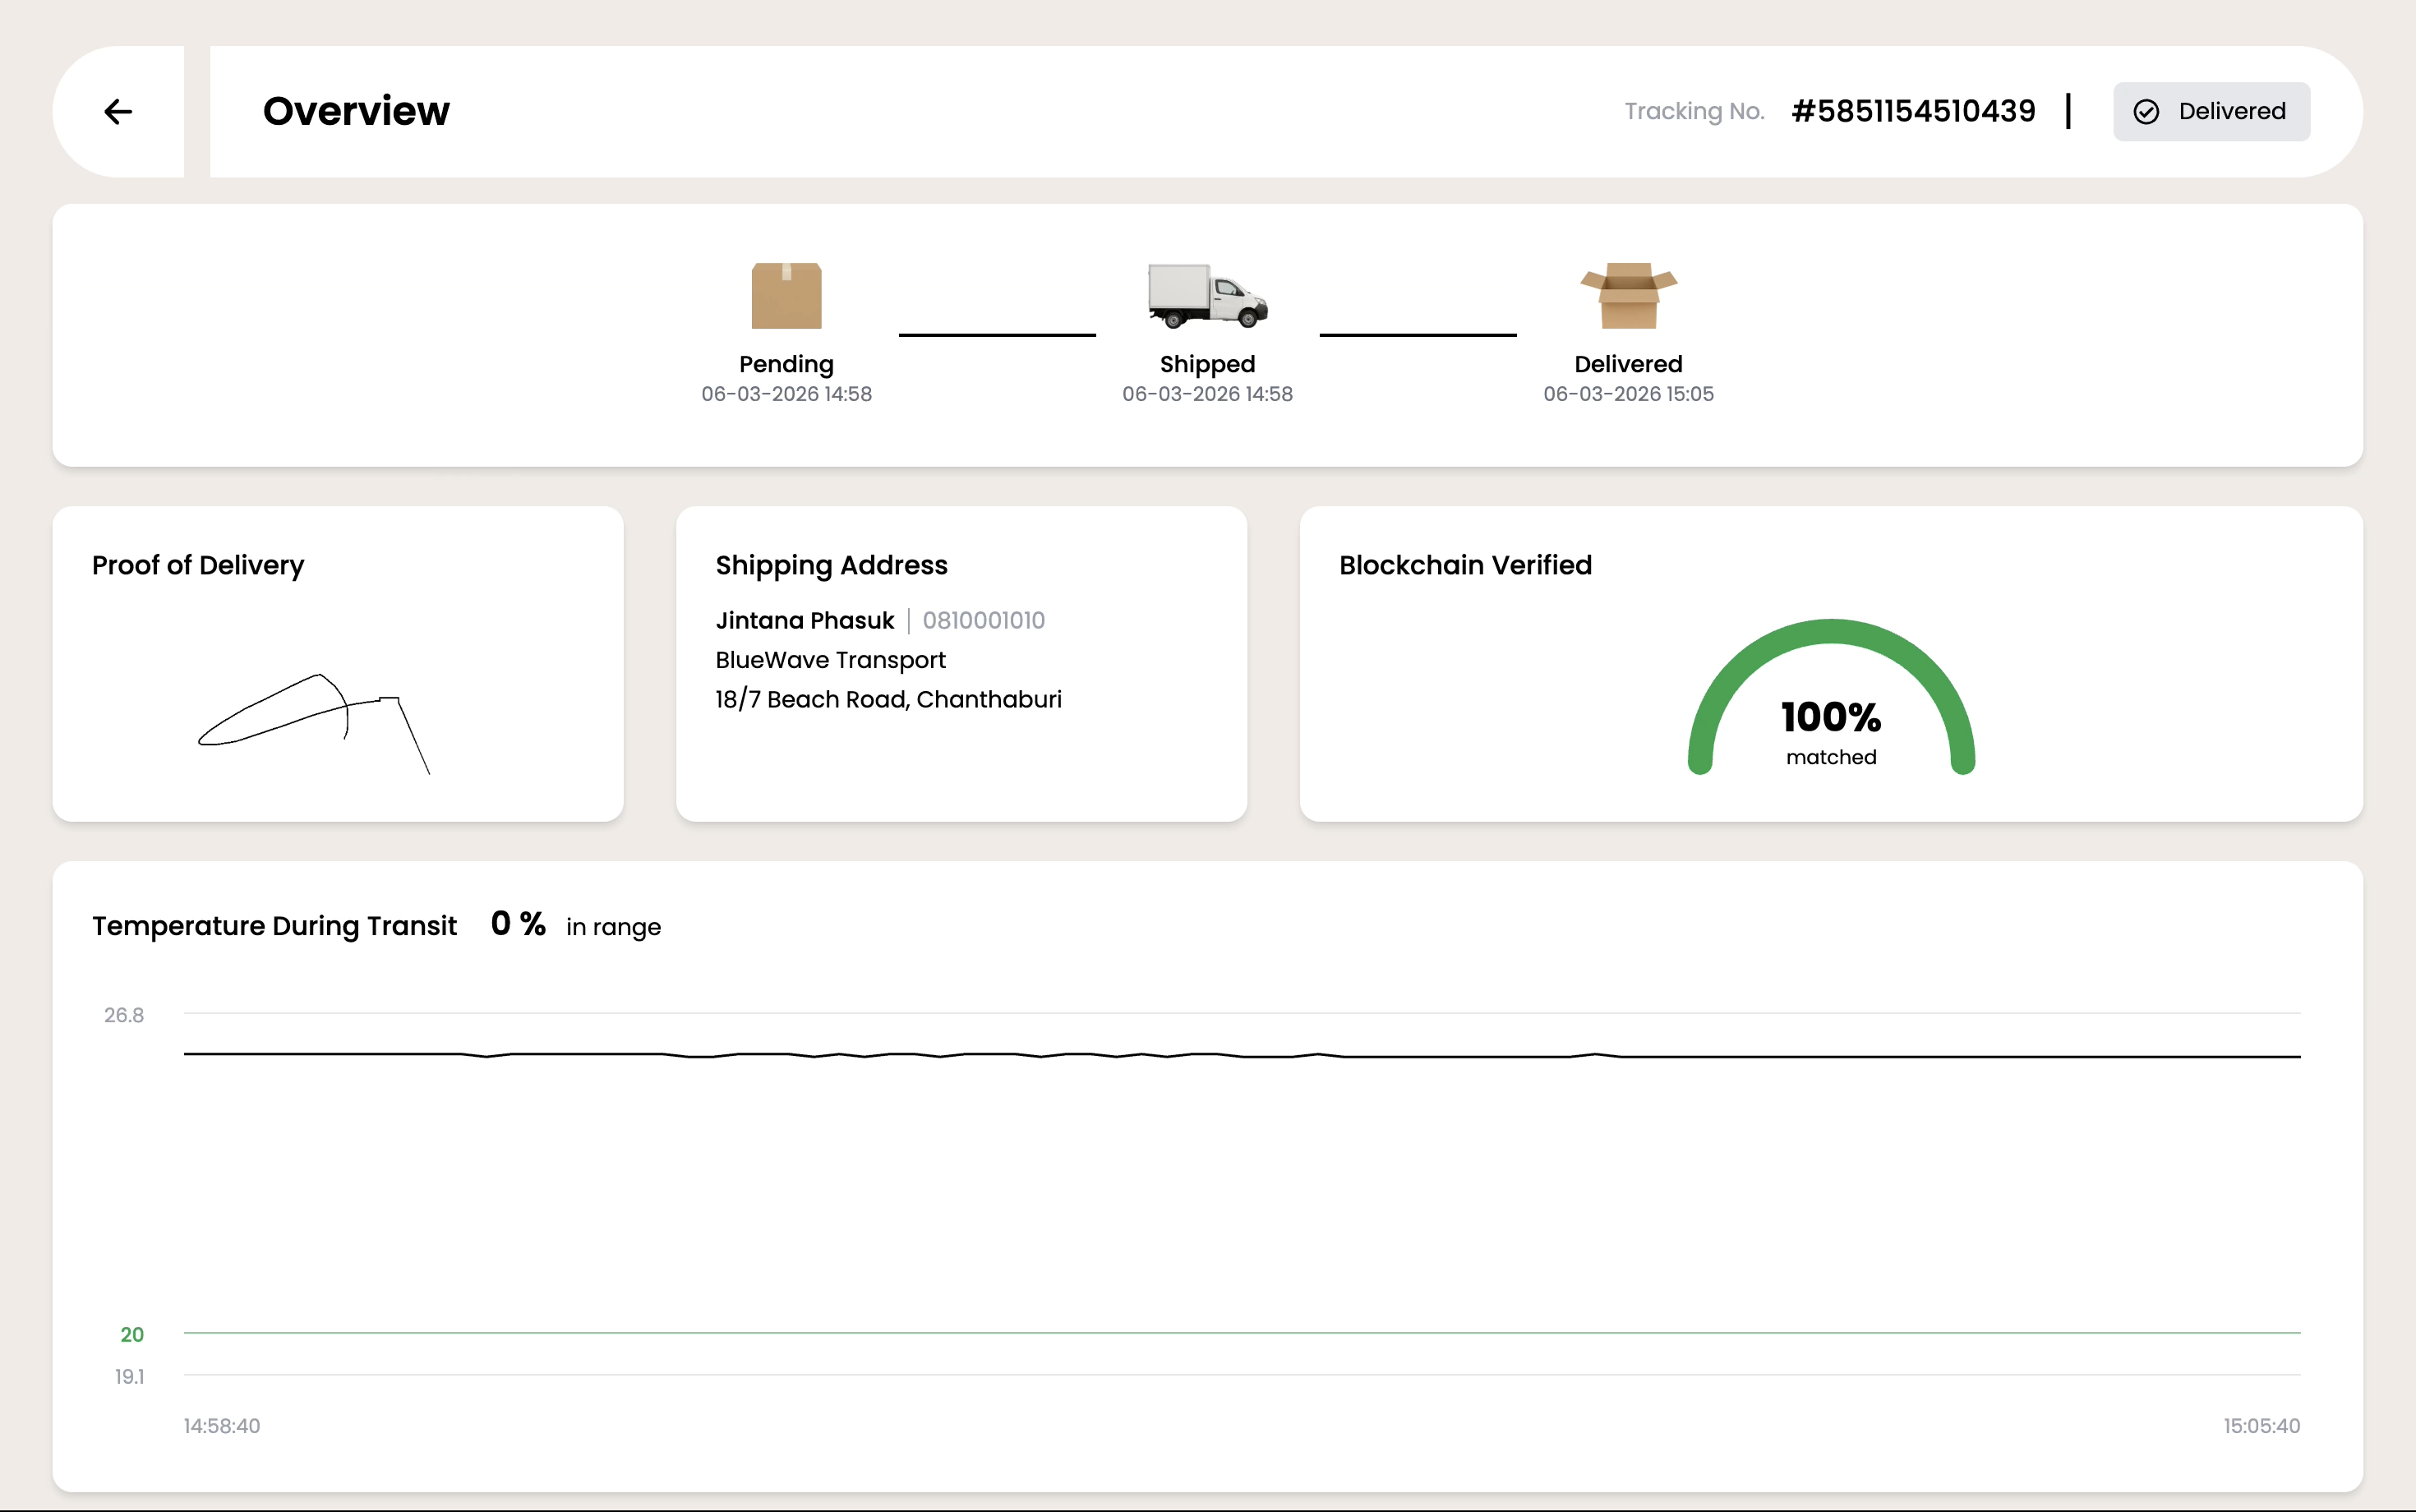
\includegraphics[width=0.8\textwidth]{overview.png}
    \caption{หน้าสรุปข้อมูลการขนส่งและการยืนยันความถูกต้องผ่านบล็อกเชน}
    \label{fig:ui_user_overview}
\end{figure}
\end{minipage}


\subsection{ส่วนของผู้ดูแลระบบ}
ส่วนนี้ถูกออกแบบมาสำหรับเจ้าหน้าที่ดูแลระบบเพื่อบริหารจัดการพนักงานขับรถและการจัดส่งพัสดุในภาพรวม ประกอบด้วยหน้าต่างการทำงานดังนี้:

\vspace{1em}
\begin{minipage}{\linewidth}
\noindent \textbf{1. หน้าเพิ่มข้อมูลคนขับรถ} \\
สำหรับเพิ่มรายชื่อและรายละเอียดของคนขับรถคนใหม่เข้าสู่ระบบ เพื่อเตรียมความพร้อมในการจัดส่งพัสดุ
\begin{figure}[H]
    \centering
    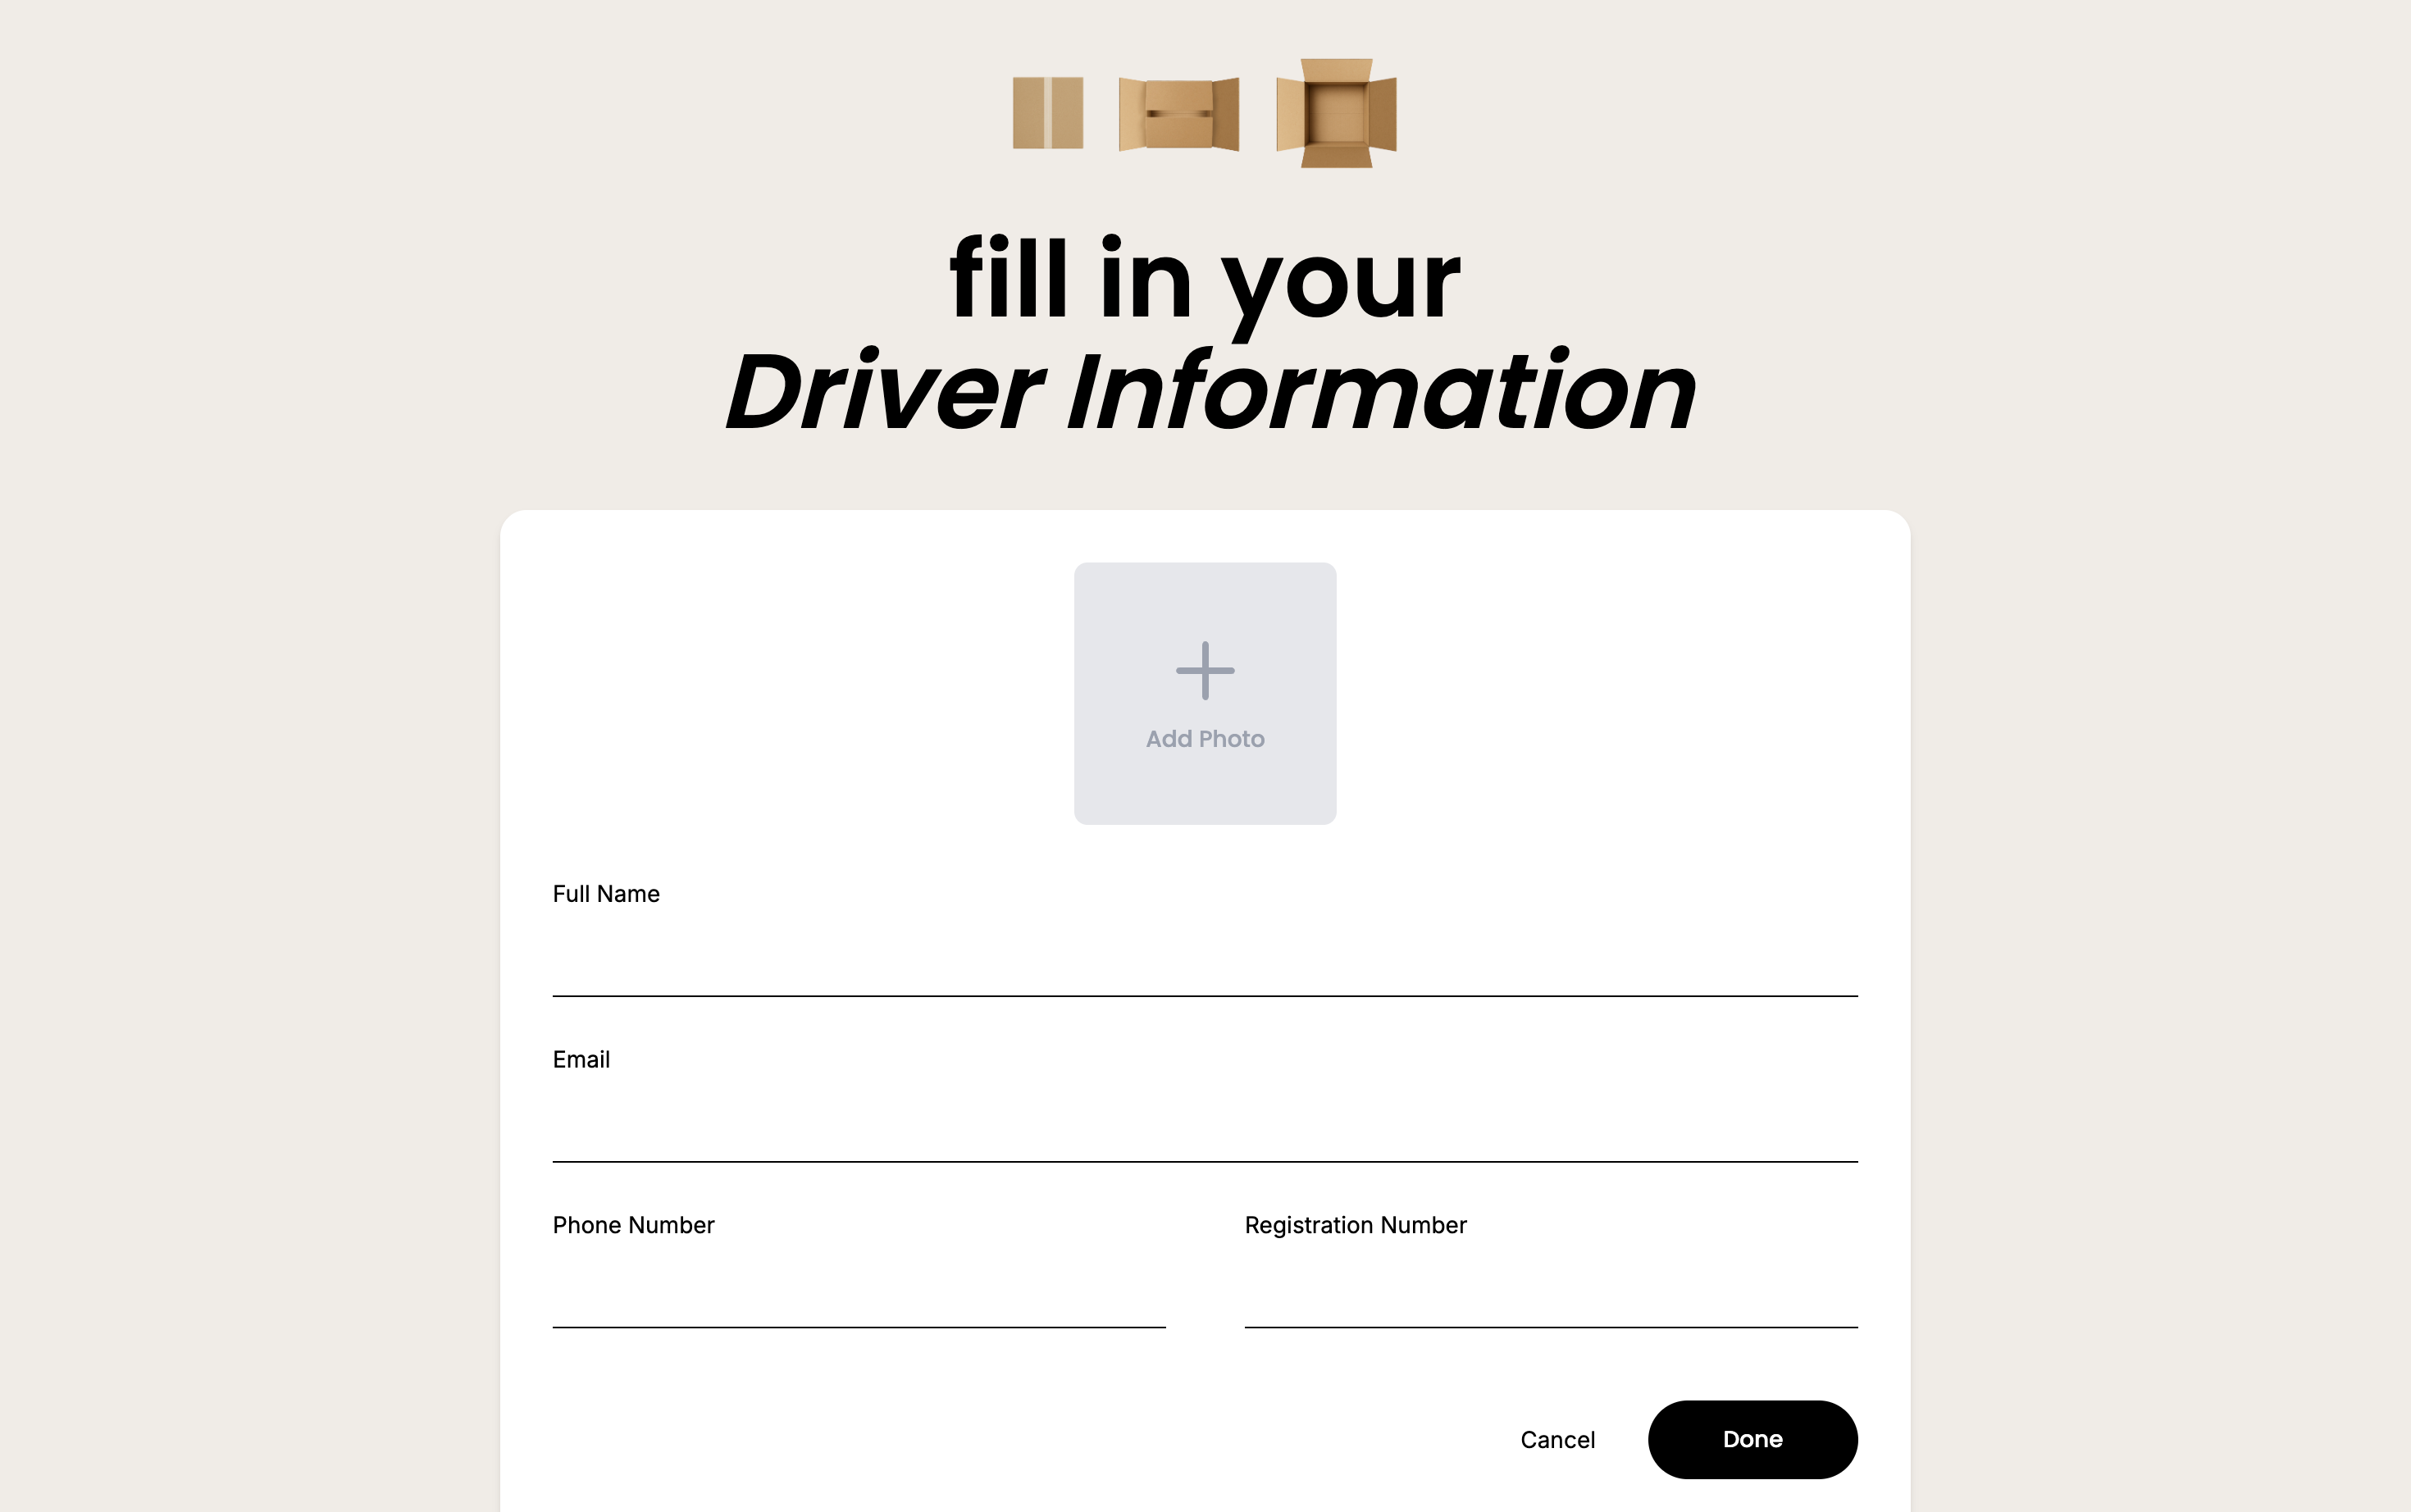
\includegraphics[width=0.8\textwidth]{admin_add_driver.png}
    \caption{หน้าเพิ่มข้อมูลคนขับรถ}
    \label{fig:ui_admin_add_driver}
\end{figure}
\end{minipage}

\vspace{1em}
\begin{minipage}{\linewidth}
\noindent \textbf{2. หน้าแสดงข้อมูลคนขับและพัสดุที่กำลังจัดส่ง} \\
สำหรับดูรายชื่อคนขับทั้งหมด พร้อมทั้งตรวจสอบพัสดุที่แต่ละคนกำลังรับผิดชอบจัดส่งอยู่ในขณะนั้น
\begin{figure}[H]
    \centering
    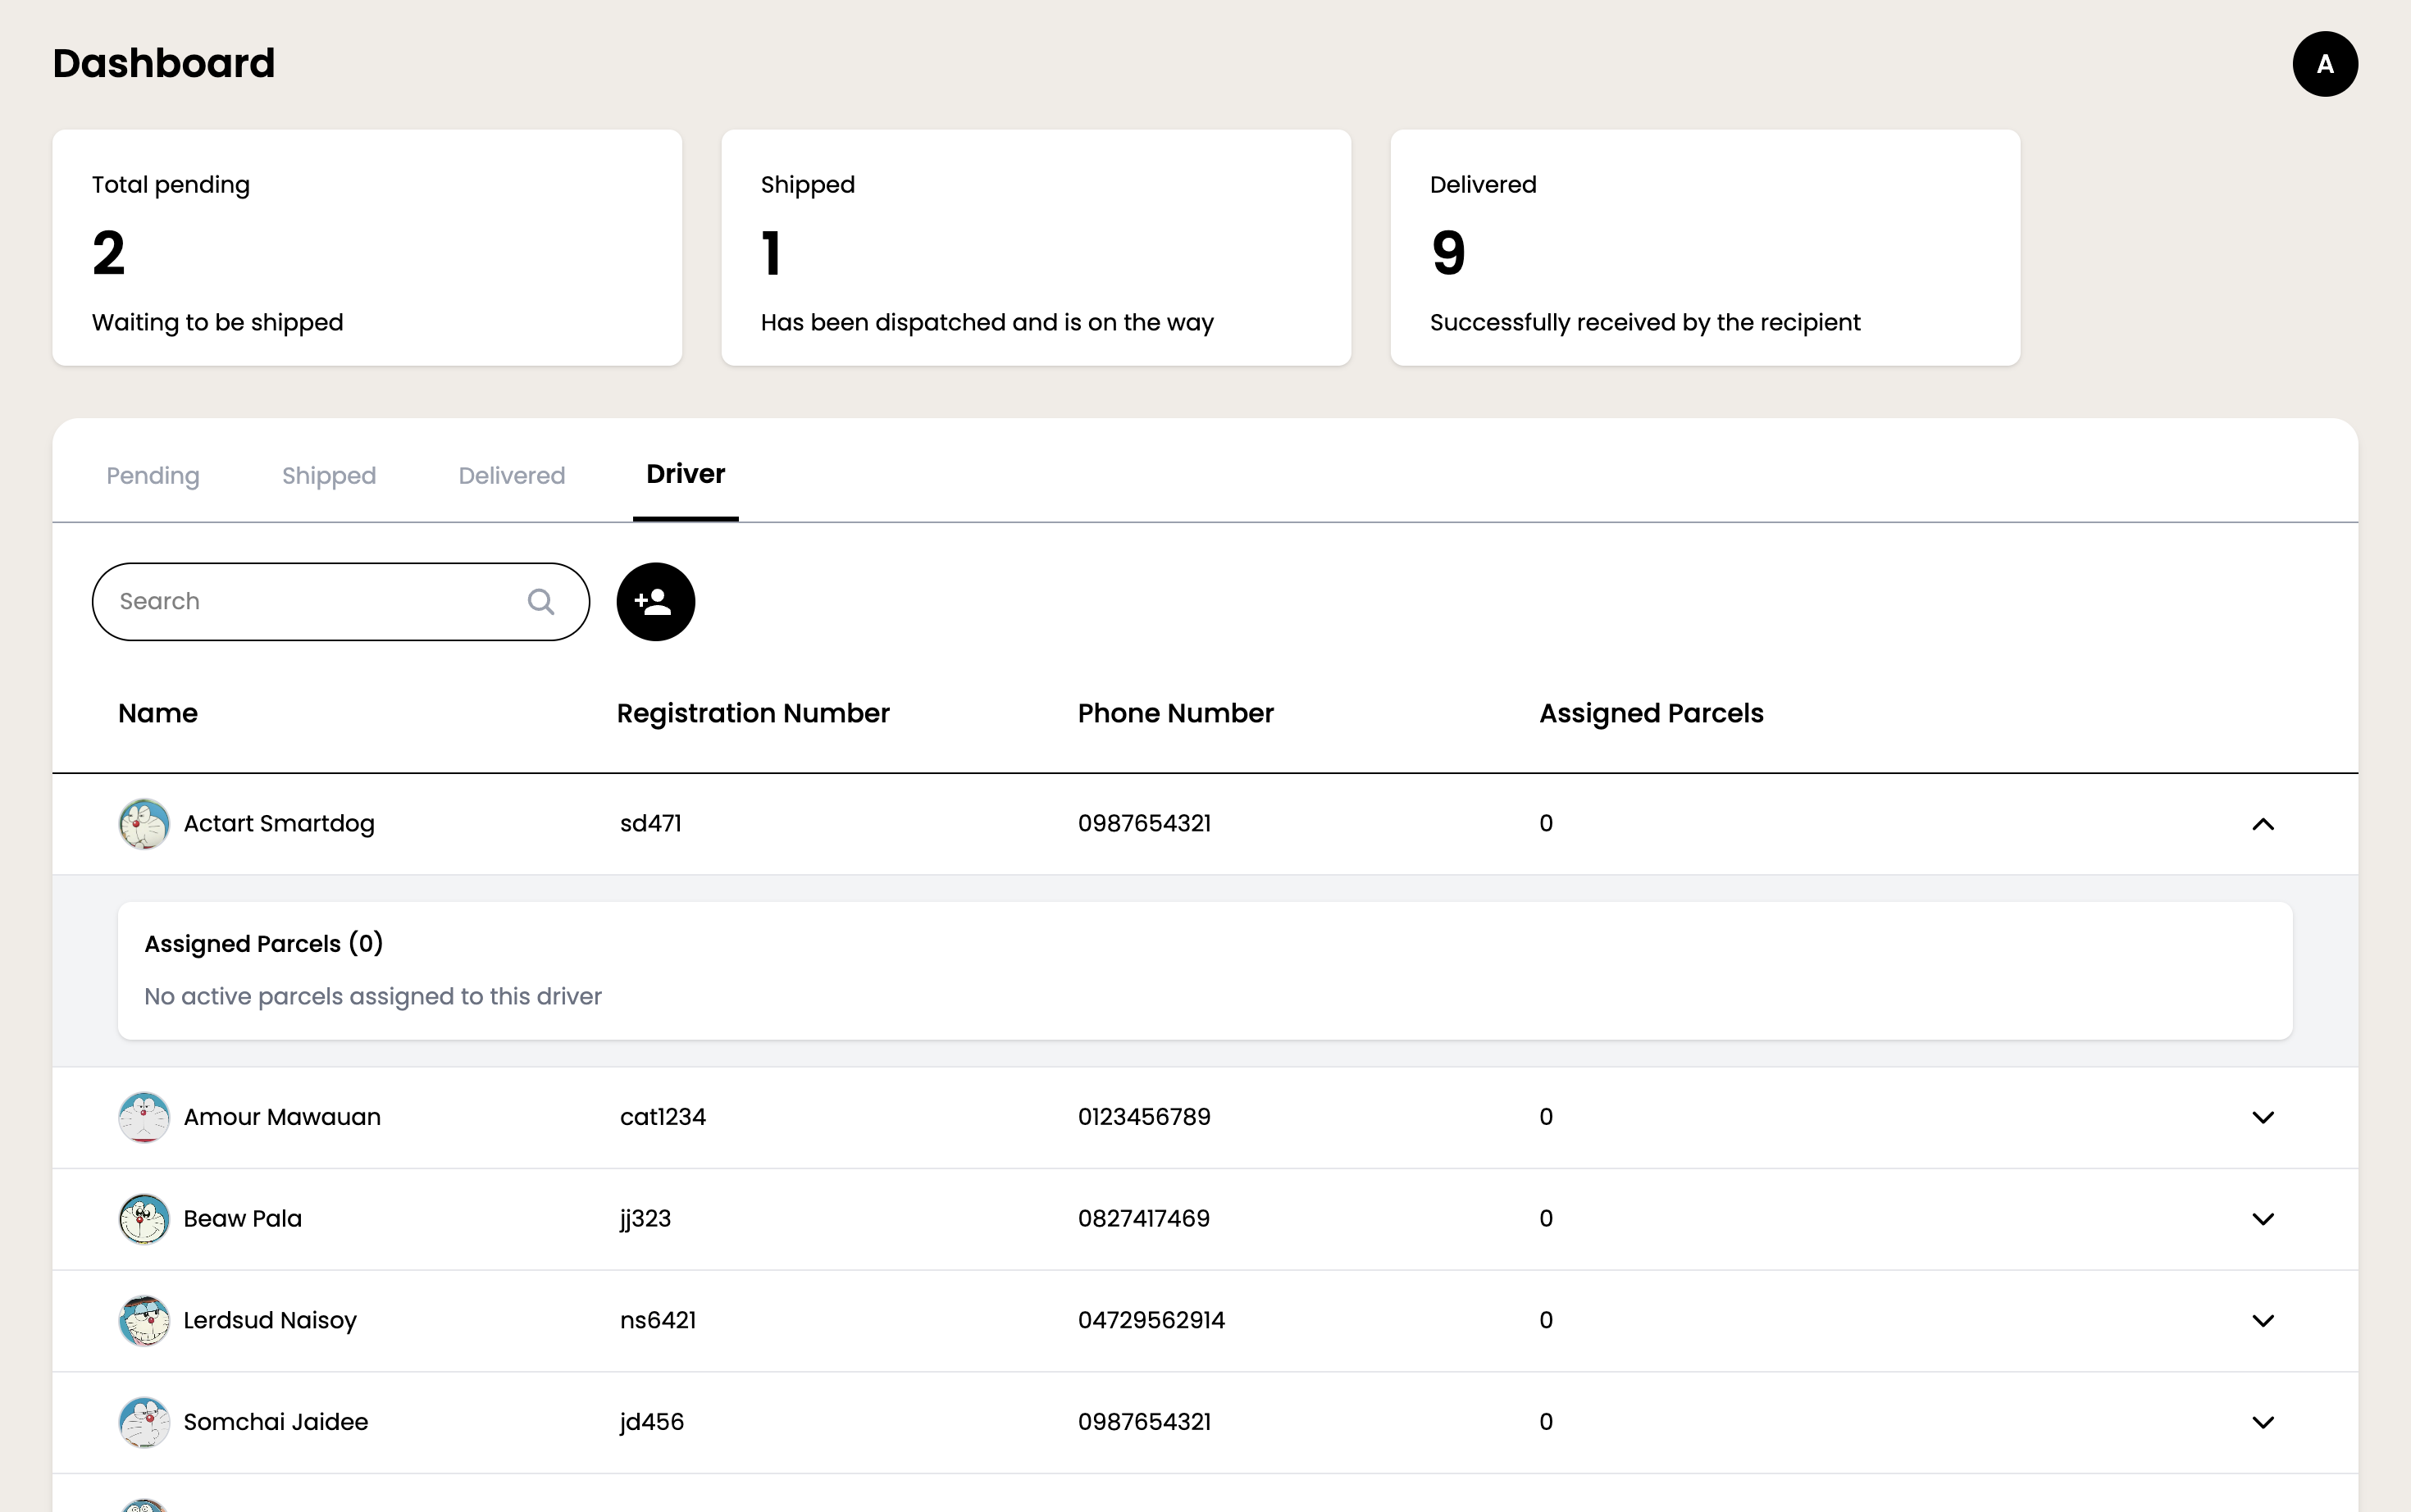
\includegraphics[width=0.8\textwidth]{admin_driver_list.png}
    \caption{หน้าแสดงข้อมูลคนขับและพัสดุที่กำลังจัดส่ง}
    \label{fig:ui_admin_driver_list}
\end{figure}
\end{minipage}

\vspace{1em}
\begin{minipage}{\linewidth}
\noindent \textbf{3. หน้าพัสดุที่รอการจัดสรรคนขับ} \\
สำหรับแสดงรายการพัสดุที่เข้าสู่ระบบ และกำลังรอให้ผู้ดูแลระบบเลือกคนขับรถที่เหมาะสมเพื่อเริ่มต้นการจัดส่ง
\begin{figure}[H]
    \centering
    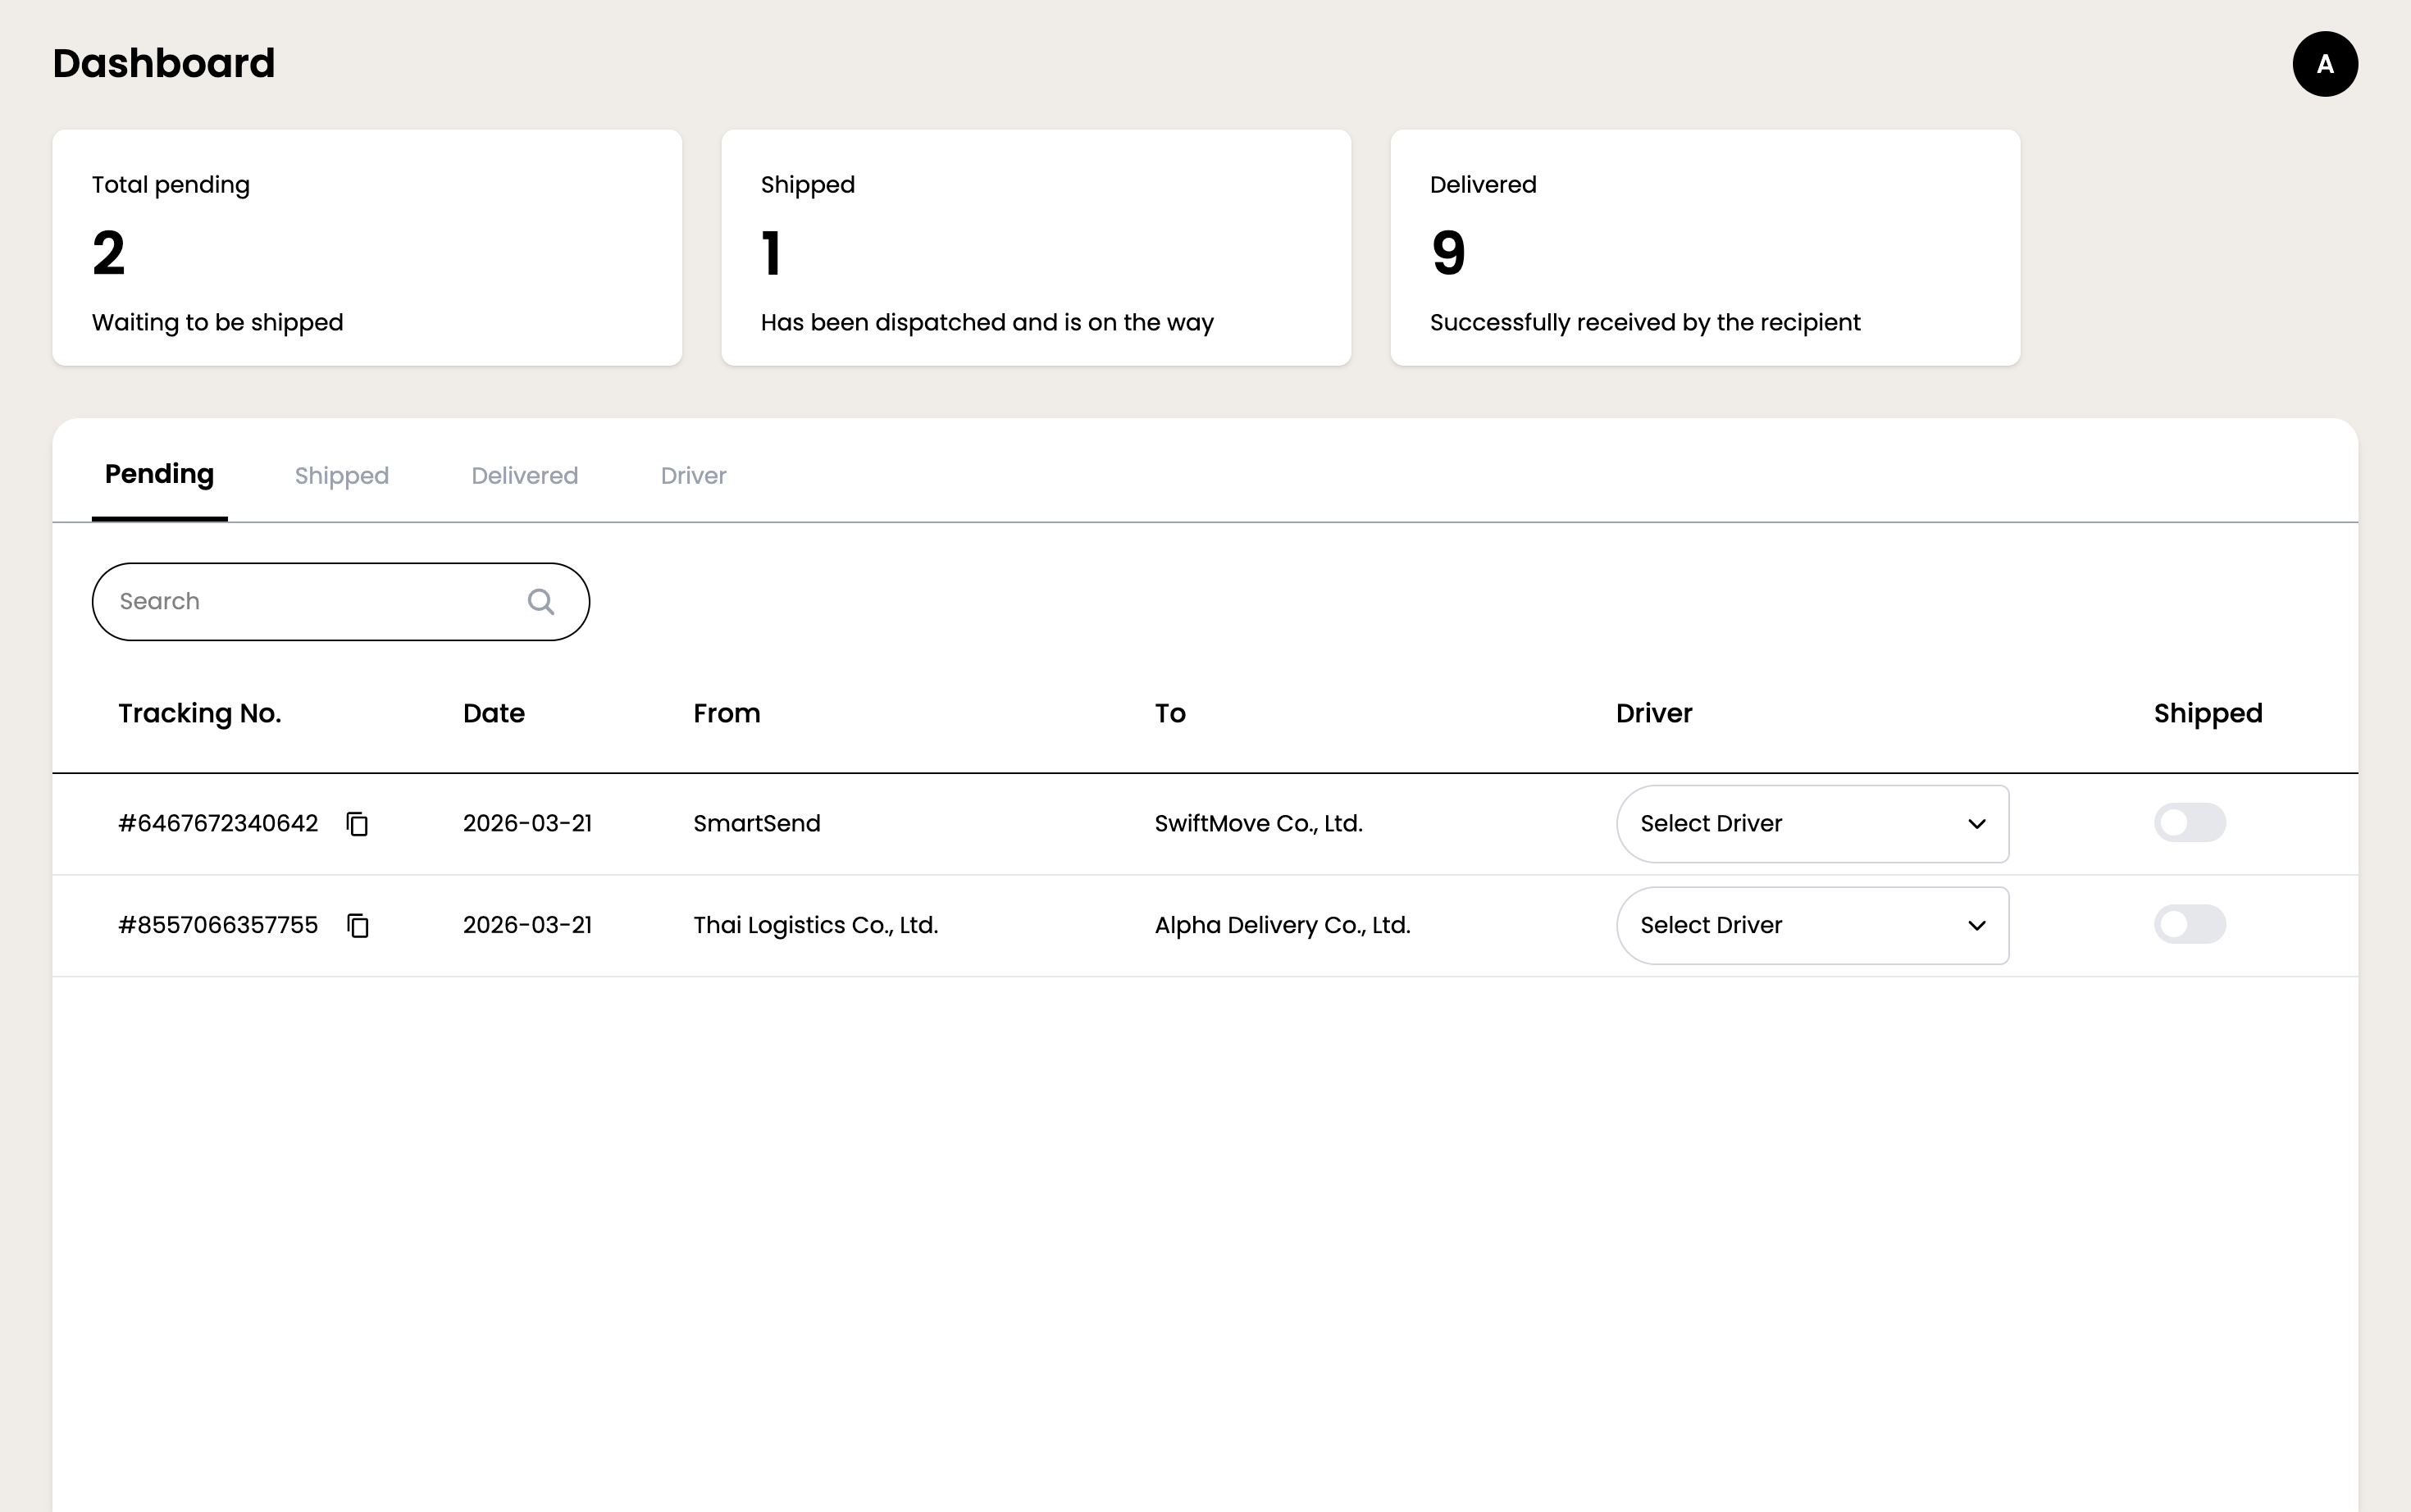
\includegraphics[width=0.8\textwidth]{admin_pending_parcels.png}
    \caption{หน้าพัสดุที่รอเลือกคนขับเพื่อเริ่มการจัดส่ง}
    \label{fig:ui_admin_pending_parcels}
\end{figure}
\end{minipage}

\vspace{1em}
\begin{minipage}{\linewidth}
\noindent \textbf{4. หน้าอัปเดตสถานะการจัดส่ง} \\
สำหรับให้ผู้ดูแลระบบเข้ามาปรับเปลี่ยนสถานะของพัสดุในระบบ เช่น เปลี่ยนจากสถานะอยู่ระหว่างการจัดส่ง (Shipped) เป็นจัดส่งสำเร็จแล้ว (Delivered)
\begin{figure}[H]
    \centering
    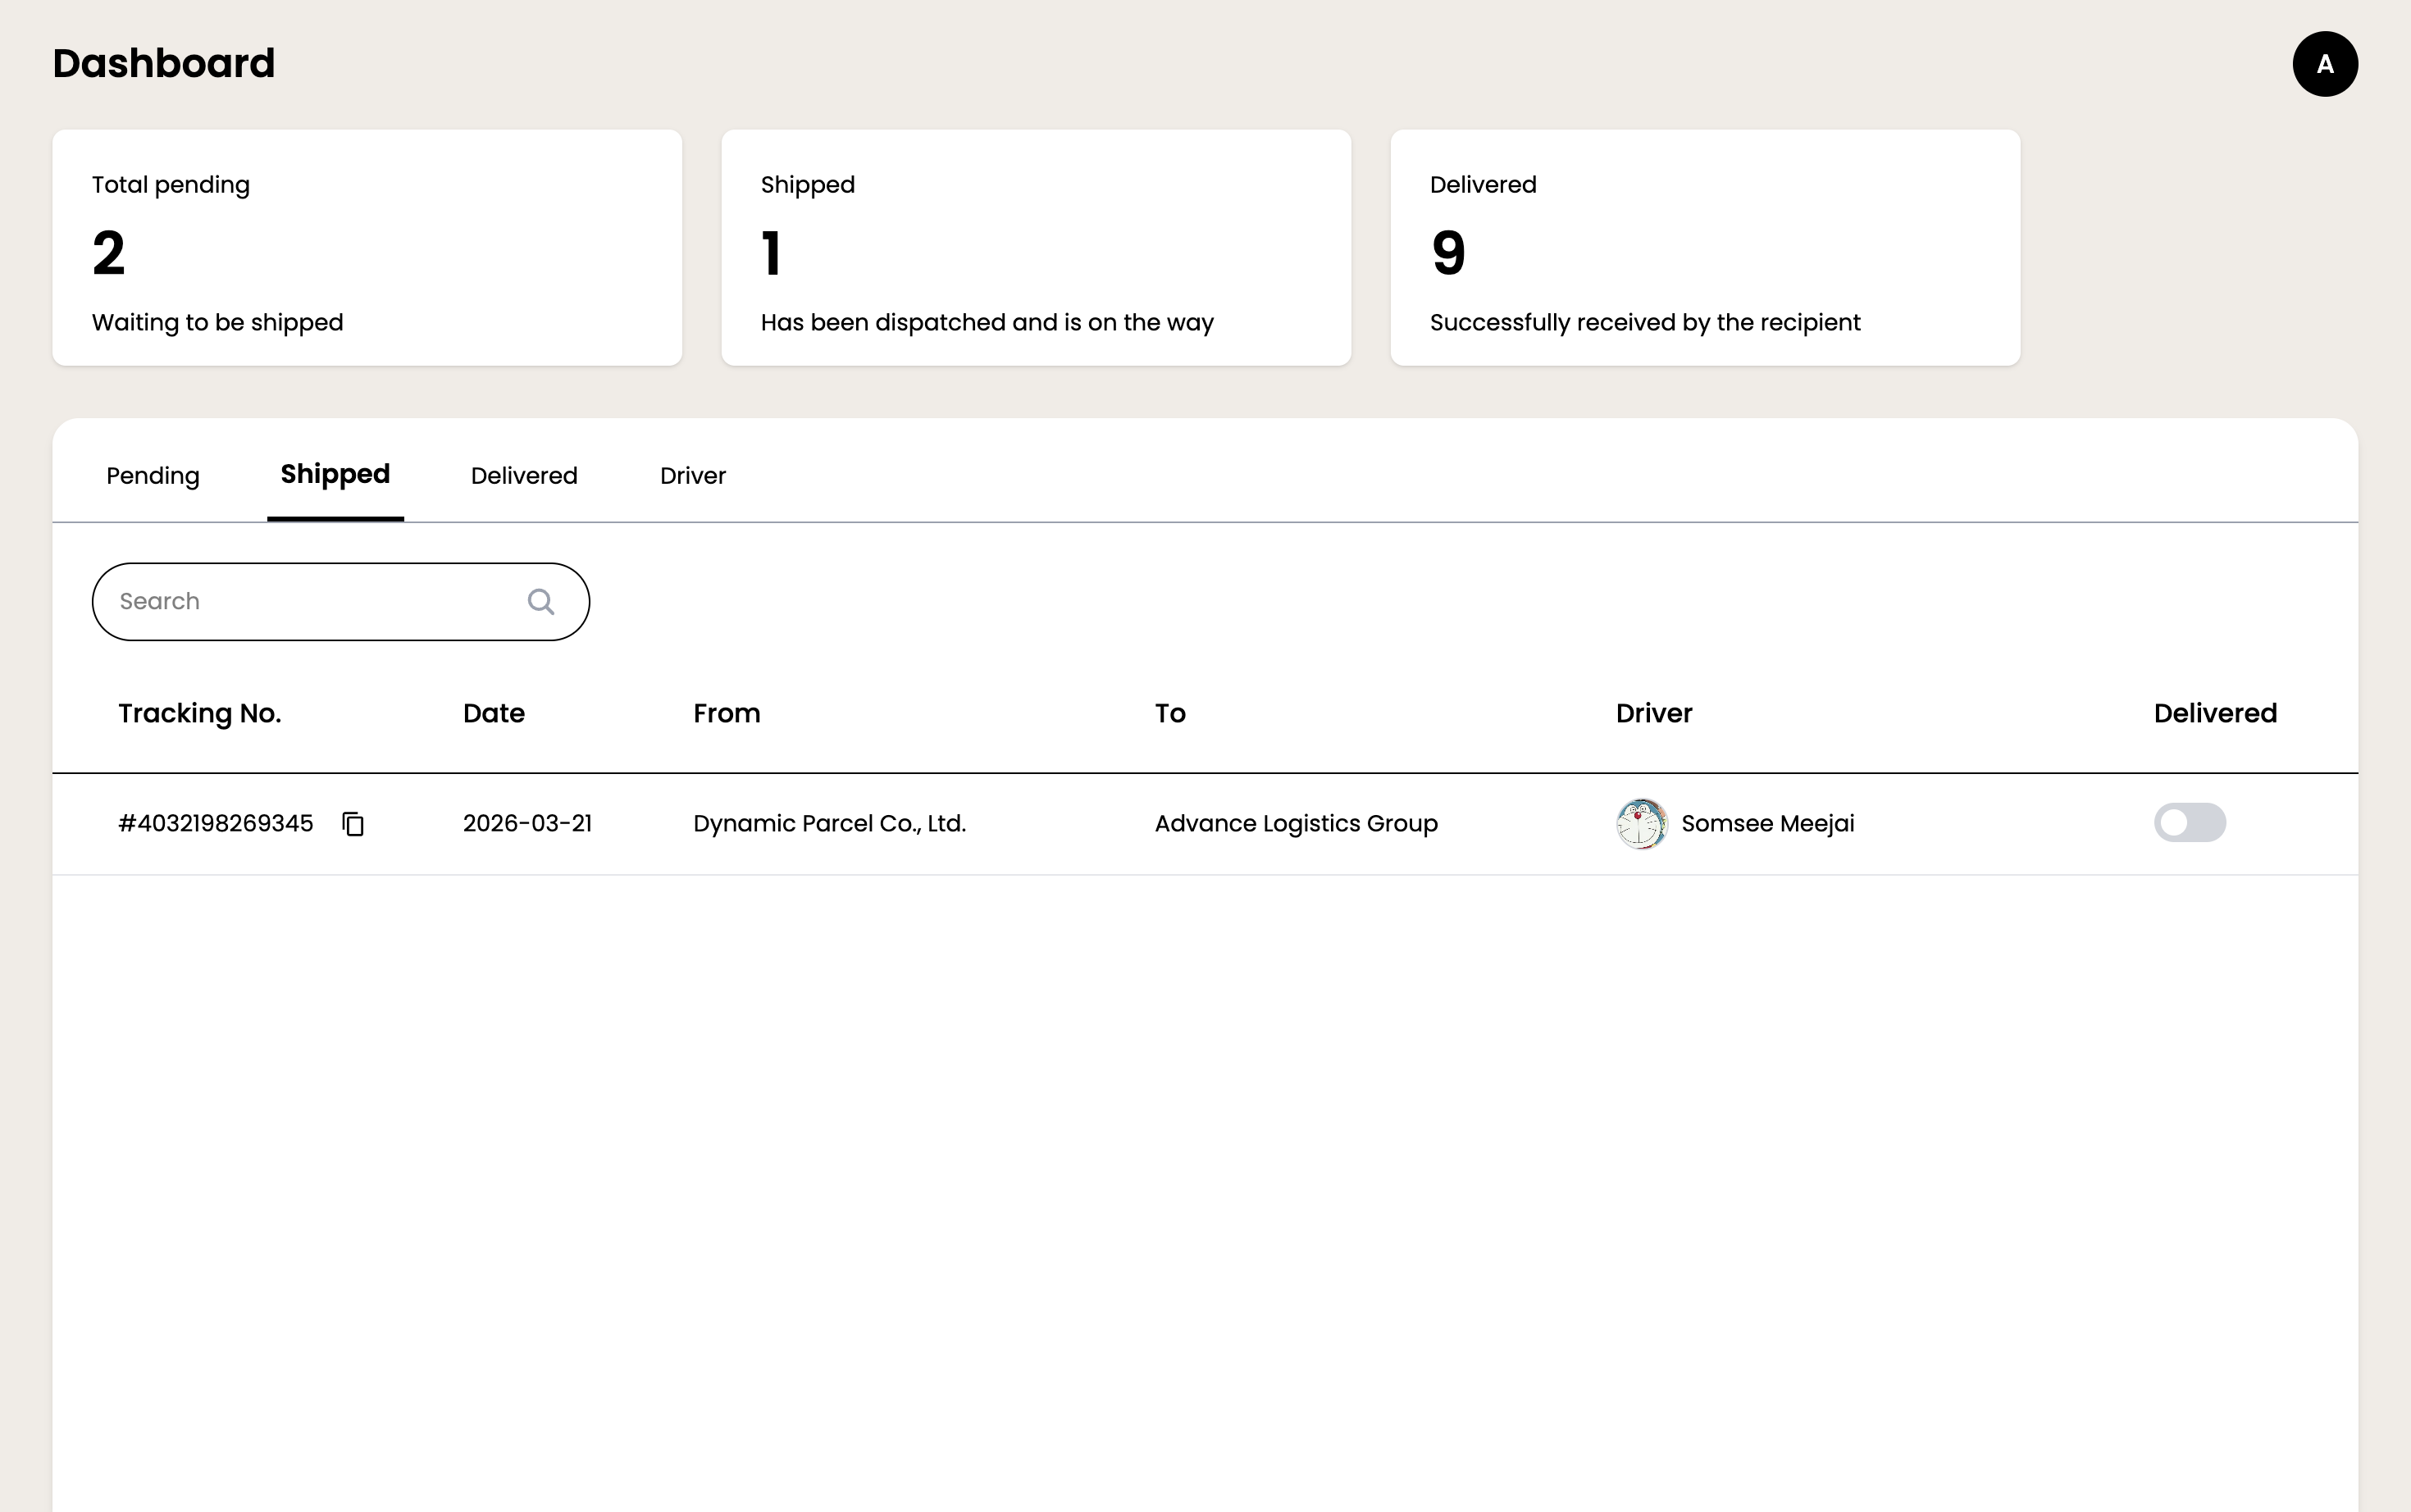
\includegraphics[width=0.8\textwidth]{admin_update_status.png}
    \caption{หน้าเปลี่ยนสถานะพัสดุ}
    \label{fig:ui_admin_update_status}
\end{figure}
\end{minipage}

\vspace{1em}
\begin{minipage}{\linewidth}
\noindent \textbf{5. หน้าประวัติพัสดุที่จัดส่งเสร็จสิ้น} \\
สำหรับดูภาพรวมและตรวจสอบข้อมูลย้อนหลังของพัสดุทั้งหมดที่มีการจัดส่งเสร็จสิ้นสมบูรณ์แล้วในระบบ
\begin{figure}[H]
    \centering
    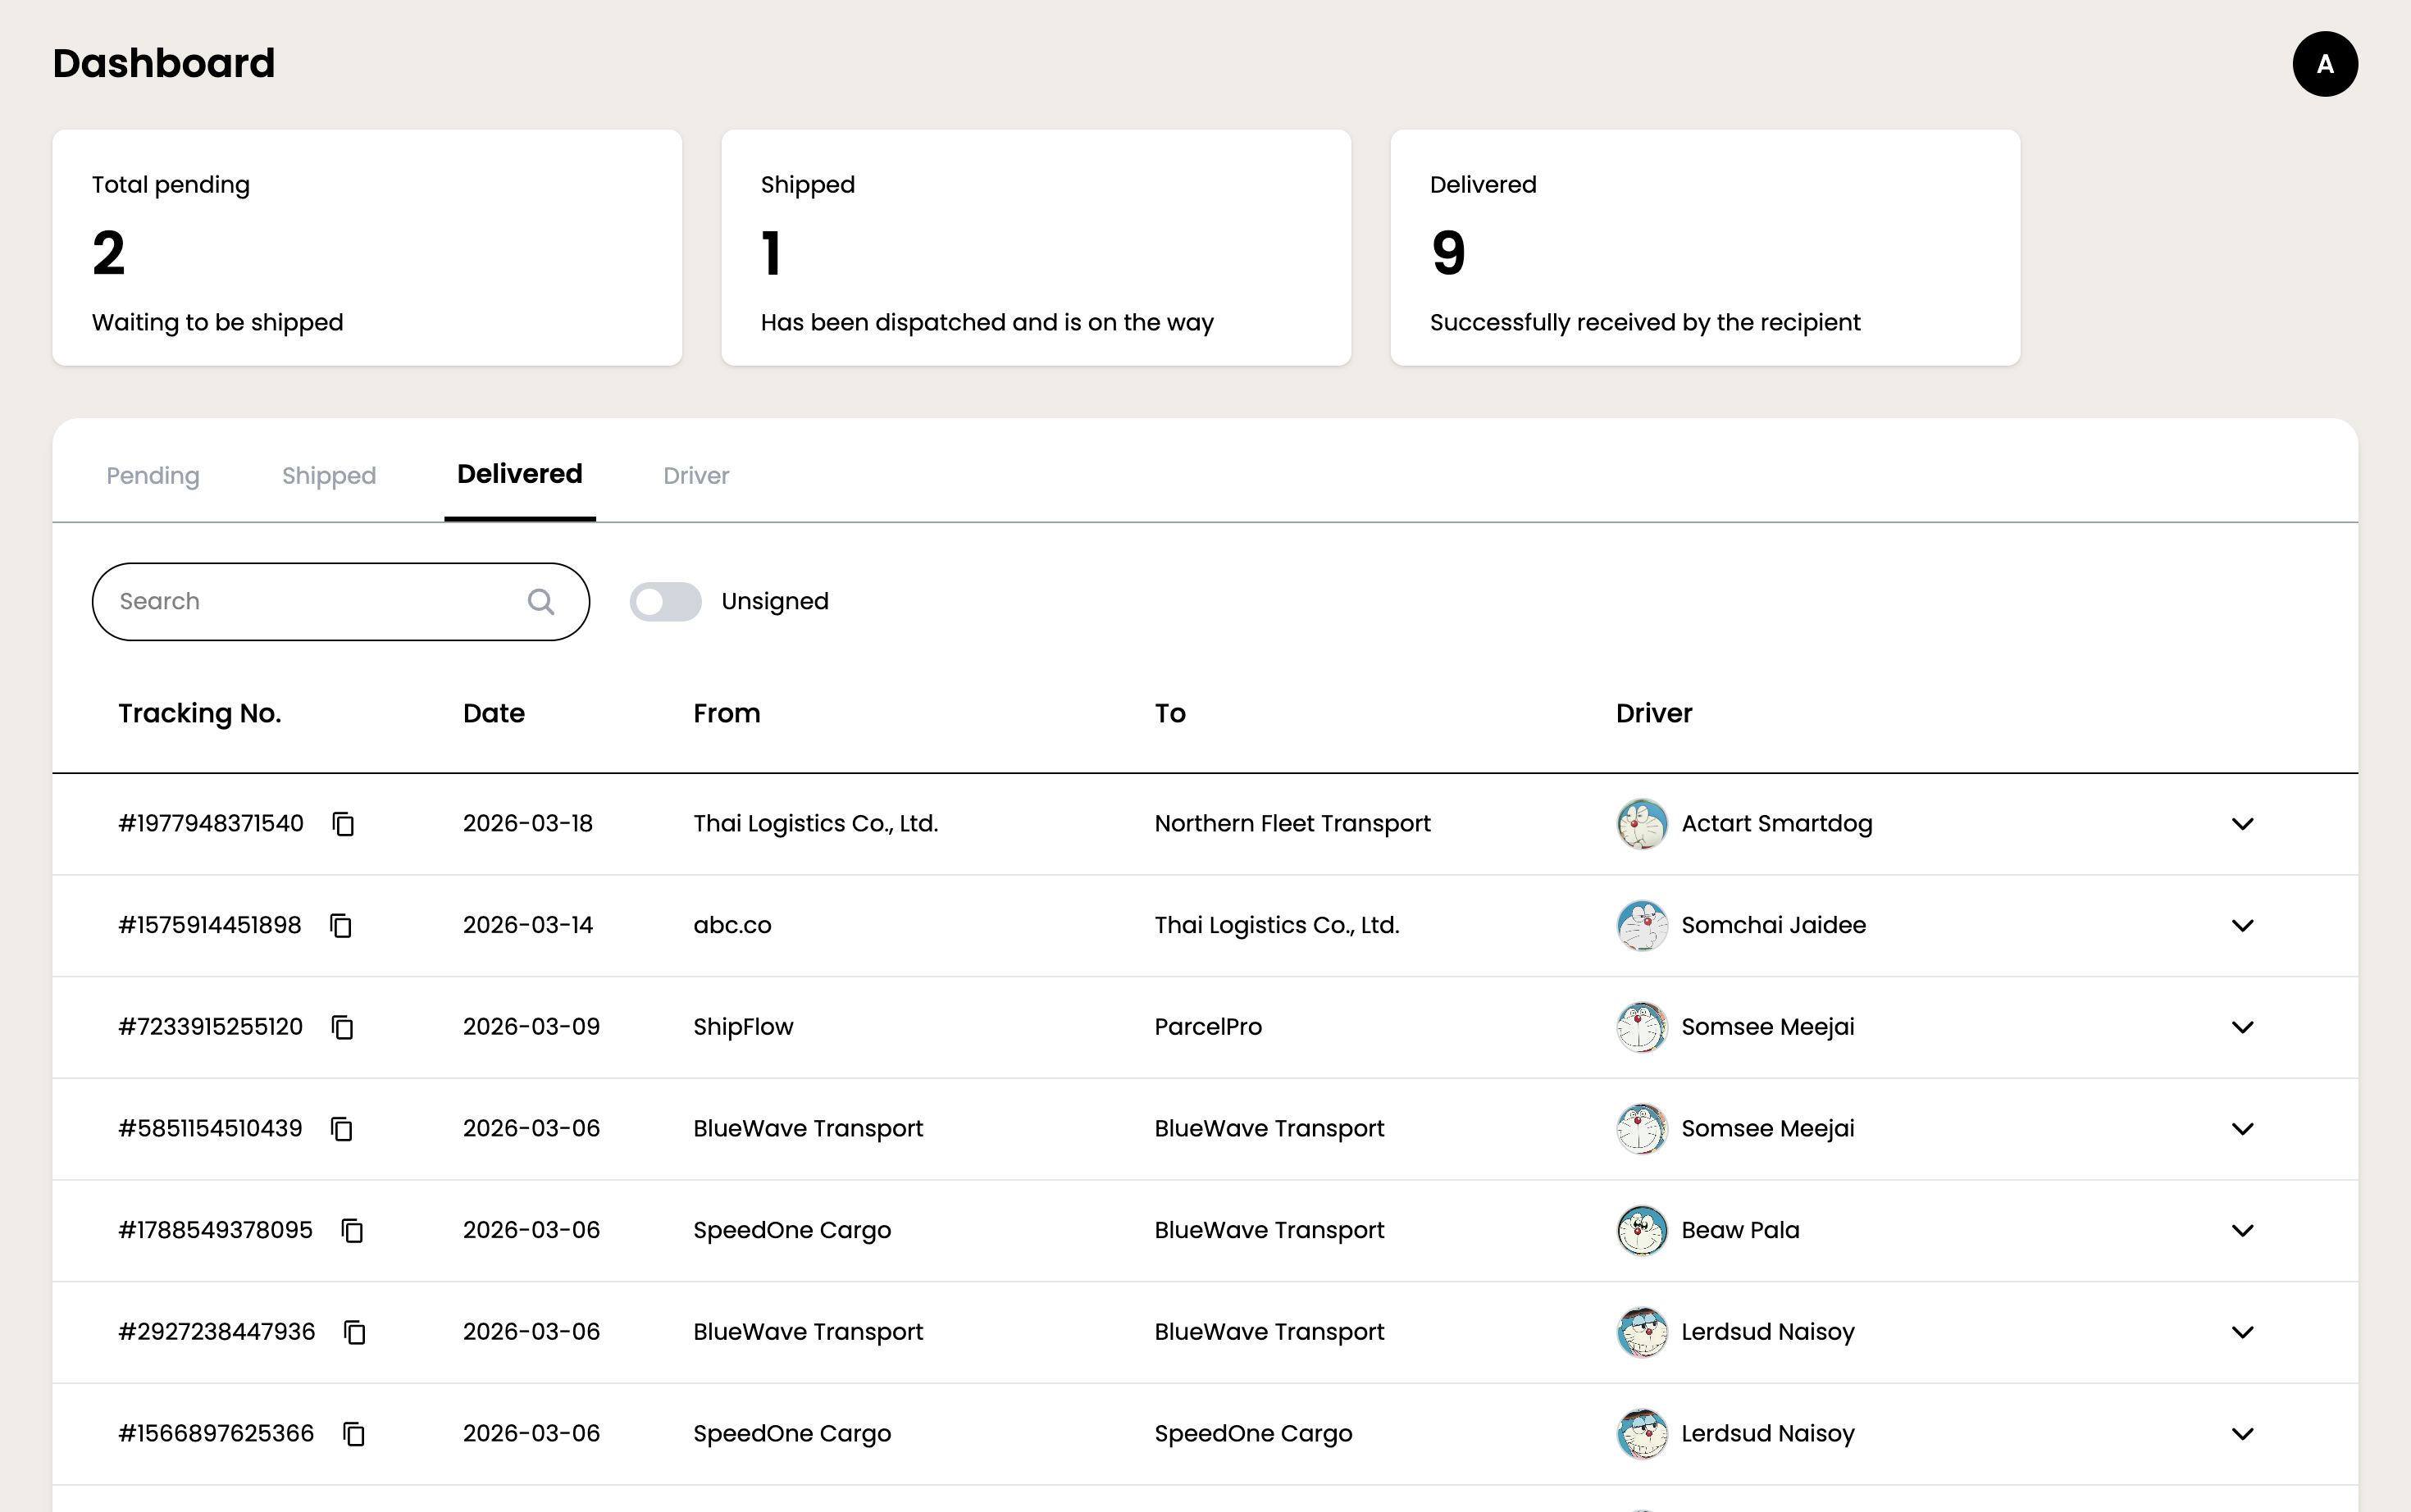
\includegraphics[width=0.8\textwidth]{admin_delivery_history.png}
    \caption{หน้าประวัติพัสดุที่เคยจัดส่งเสร็จแล้วทั้งหมด}
    \label{fig:ui_admin_delivery_history}
\end{figure}
\end{minipage}
\chapter{\ifproject%
% \ifenglish Experimentation and Results\else การทดลองและผลลัพธ์\fi
% \else%
\ifenglish System Evaluation\else การประเมินระบบ\fi
\fi}

\section{การประเมินประสิทธิภาพของอุปกรณ์ไอโอที}

ในปัจจุบัน อุปกรณ์ไอโอทีได้รับความนิยมอย่างแพร่หลาย โดยเฉพาะในด้านการตรวจวัดสิ่งแวดล้อม เช่น การวัดอุณหภูมิ ความชื้นและคุณภาพอากาศเพื่อให้มั่นใจว่าอุปกรณ์สามารถทำงานได้อย่างมีประสิทธิภาพ การประเมินประสิทธิภาพของอุปกรณ์จึงเป็นสิ่งสำคัญ 
การศึกษานี้มีวัตถุประสงค์เพื่อประเมินประสิทธิภาพของเซนเซอร์วัดอุณหภูมิที่เชื่อมต่อกับ บอร์ด KidBright โดยพิจารณาจากปัจจัยสำคัญ ได้แก่ ความแม่นยำในการวัด ความเร็วในการตอบสนอง และความเสถียรของระบบ 
การทดสอบเซนเซอร์วัดอุณหภูมิที่เชื่อมต่อกับบอร์ด KidBright ในครั้งนี้ใช้วิธีการดังต่อไปนี้ 

\begin{enumerate}
    \item การทดสอบความแม่นยำ 
    \begin{itemize}
        \item ใช้เซนเซอร์วัดอุณหภูมิร่วมกับบอร์ด KidBright ในการเก็บค่าข้อมูลอุณหภูมิทุกๆ 1 วินาที 
    \end{itemize}
    \item การทดสอบความเร็วในการตอบสนอง 
    \begin{itemize}
        \item นำเซนเซอร์จากอุณหภูมิห้องไปยังแหล่งความเย็น (เช่น น้ำเย็น) และจับเวลาในการเปลี่ยนค่าของเซนเซอร์ 
        \item ทดสอบซ้ำหลายครั้ง 
    \end{itemize}
    \item การทดสอบความเสถียร 
    \begin{itemize}
        \item เก็บค่าข้อมูลเป็นระยะเวลา 4 ชั่วโมง และวิเคราะห์ว่าค่าที่ได้มีความผันผวนมากน้อยเพียงใด 
    \end{itemize}
    \item การทดสอบการใช้พลังงาน
    \begin{itemize}
        \item วัดกระแสไฟฟ้าที่เซนเซอร์และบอร์ด KidBright ใช้งาน โดยใช้เครื่องวัดพลังงานไฟฟ้า 
    \end{itemize}
\end{enumerate}

\section{การประเมินประสิทธิภาพของ Hyperledger Fabric} 

Hyperledger Fabric เป็นหนึ่งในแพลตฟอร์มบล็อกเชนที่ได้รับความนิยมในอุตสาหกรรม โดยมีคุณสมบัติสำคัญ เช่น ความสามารถในการควบคุมสิทธิ์การเข้าถึงข้อมูล ความปลอดภัย และการบันทึกข้อมูลแบบไม่สามารถแก้ไขได้ (Immutable Ledger) ซึ่งเหมาะสำหรับการใช้งานด้านไอโอทที 
การศึกษานี้มีวัตถุประสงค์เพื่อ ประเมินประสิทธิภาพของ Hyperledger Fabric ในการจัดเก็บข้อมูลอุณหภูมิจากเซนเซอร์ที่เชื่อมต่อกับบอร์ด KidBright ในแบบเรียลไทม์ โดยวัดประสิทธิภาพในด้าน ความเร็วในการเขียนข้อมูล, ความเร็วในการอ่านข้อมูล, ความสามารถในการรองรับธุรกรรมพร้อมกัน และความถูกต้องของข้อมูล 
การทดสอบ Hyperledger Fabric ในการจัดเก็บข้อมูลอุณหภูมิจากเซนเซอร์ที่เชื่อมต่อกับบอร์ด KidBright ในแบบเรียลไทม์ ในครั้งนี้ใช้วิธีการดังต่อไปนี้

\begin{enumerate}
    \item การตั้งค่าระบบทดสอบ 
    \begin{itemize}
        \item ใช้บอร์ด KidBright เชื่อมต่อกับเซนเซอร์วัดอุณหภูมิ (DS18B20) ส่งข้อมูลอุณหภูมิไปยัง Hyperledger Fabric ผ่าน MQTT หรือ HTTP API 
    \end{itemize}
    \item การทดสอบความเร็วในการเขียนข้อมูล 
    \begin{itemize}
        \item วัดระยะเวลาที่ใช้ตั้งแต่การส่งข้อมูลจาก KidBright จนถึงการบันทึกสำเร็จในบล็อกเชน 
    \end{itemize}
    \item การทดสอบความเร็วในการอ่านข้อมูล 
    \begin{itemize}
        \item ส่งคำขอดึงข้อมูลอุณหภูมิจาก Hyperledger Fabric และวัดระยะเวลาที่ใช้ 
    \end{itemize}
    \item การทดสอบความสามารถในการรองรับธุรกรรมพร้อมกัน (Throughput Test) 
    \begin{itemize}
        \item ใช้ Hyperledger Caliper ในการจำลองการส่งข้อมูลจากเซนเซอร์หลายตัว 
        \item วัดค่า TPS สูงสุดที่ระบบสามารถรองรับได้ 
    \end{itemize}
    \item การทดสอบความถูกต้องของข้อมูล 
    \begin{itemize}
        \item เปรียบเทียบค่าที่ได้รับจาก Hyperledger Fabric กับค่าจริงที่ส่งจากบอร์ด KidBright 
        \item ตรวจสอบว่ามีความคลาดเคลื่อนของข้อมูลหรือไม่ 
    \end{itemize}
\end{enumerate} 

\ifproject
% \chapter{\ifenglish Conclusions and Discussions\else บทสรุปและข้อเสนอแนะ\fi}

\section{\ifenglish Conclusions\else สรุปผล\fi}

ปริญญานิพนธ์ฉบับนี้ได้นำเสนอการพัฒนา "ระบบจัดการห่วงโซ่อุปทานด้วยบล็อกเชนและไอโอที " โดยมีวัตถุประสงค์เพื่อยกระดับความปลอดภัยและความน่าเชื่อถือของข้อมูลอุณหภูมิในกระบวนการขนส่ง จากผลการดำเนินงานสามารถสรุปได้ว่า ระบบที่พัฒนาขึ้นสามารถทำงานได้บรรลุตามวัตถุประสงค์ทุกประการ 

ระบบสามารถอ่านค่าอุณหภูมิผ่านอุปกรณ์ตรวจวัดและส่งข้อมูลตามเวลาจริงผ่านโปรโตคอลการสื่อสาร โดยมีความหน่วงเวลาเฉลี่ยเพียง 1.2 วินาที ข้อมูลทั้งหมดถูกบันทึกลงในเครือข่ายบล็อกเชนแบบอนุญาต ซึ่งรับประกันความสมบูรณ์ของข้อมูลได้ร้อยละ 100 โดยไม่มีการสูญหายหรือถูกดัดแปลงแก้ไข นอกจากนี้หน้ากระดานสรุปข้อมูลยังสามารถแสดงผลข้อมูลย้อนหลังและแจ้งเตือนเมื่ออุณหภูมิออกนอกเกณฑ์ที่กำหนดได้อย่างแม่นยำ

\textbf{ข้อจำกัดของระบบ} \\
แม้ระบบจะสามารถทำงานได้ตามเกณฑ์มาตรฐาน แต่ยังมีข้อจำกัดบางประการที่พบจากการพัฒนาและทดสอบ ดังนี้
\begin{enumerate}
    \item \textbf{ข้อจำกัดด้านเครือข่ายของอุปกรณ์ฮาร์ดแวร์:} อุปกรณ์ไอโอที ที่ใช้ในโครงงานนี้ยังคงพึ่งพาการเชื่อมต่อผ่านระบบเครือข่ายไร้สาย เป็นหลัก ทำให้ไม่เหมาะกับการนำไปติดตั้งบนยานพาหนะขนส่งที่ต้องเคลื่อนที่ตลอดเวลาในพื้นที่ที่ไม่มีสัญญาณ
    \item \textbf{ข้อจำกัดด้านโครงสร้างพื้นฐานของบล็อกเชน:} ในช่วงการพัฒนาและทดสอบนี้ เครือข่ายบล็อกเชนถูกจำลองและติดตั้งรวมอยู่บนเครื่องแม่ข่ายคลาวด์เพียงโหนดเดียว แม้ในเชิงตรรกะจะมีการแยกองค์กร แต่ในเชิงกายภาพยังถือว่ามีโครงสร้างพื้นฐานแบบรวมศูนย์ ระดับหนึ่ง ซึ่งในสภาพแวดล้อมจริงควรแยกโหนดไปตามองค์กรต่าง ๆ
    \item \textbf{ข้อจำกัดด้านการแจ้งเตือน:} ระบบแจ้งเตือนในปัจจุบันเป็นการทำงานแบบตรวจสอบตามเงื่อนไขที่กำหนด เมื่ออุณหภูมิเกินค่าที่กำหนดจึงจะทำการแจ้งเตือน แต่ยังไม่มีระบบการวิเคราะห์เชิงคาดการณ์ล่วงหน้า
\end{enumerate}

\section{\ifenglish Challenges\else ปัญหาที่พบและแนวทางการแก้ไข\fi}

ในการทำโครงงานนี้ พบว่าเกิดปัญหาหลัก ๆ และได้ดำเนินการแก้ไข ดังนี้

\begin{enumerate}
    \item \textbf{ปัญหาข้อมูลตกค้างในระบบจัดการคอนเทนเนอร์}
    \begin{itemize}
        \item ปัญหาที่พบ: ในระหว่างการพัฒนาและเริ่มต้นเครือข่ายบล็อกเชนใหม่ มักพบข้อผิดพลาดทำให้ไม่สามารถสร้างช่องทางการสื่อสาร หรือบันทึกข้อมูลได้ เนื่องจากมีข้อมูลบัญชีธุรกรรมเดิมตกค้างอยู่ในระบบ
        \item แนวทางการแก้ไข: พัฒนาชุดคำสั่งสำหรับการล้างข้อมูลระดับลึก โดยบังคับหยุดและลบคอนเทนเนอร์ เครือข่าย และข้อมูลที่ตกค้าง รวมถึงลบโฟลเดอร์เก็บข้อมูลประจำตัวทิ้งทั้งหมด เพื่อให้ระบบสามารถสร้างข้อมูลการระบุตัวตนและบล็อกเริ่มต้นใหม่ได้อย่างสมบูรณ์
    \end{itemize}
    \item \textbf{ปัญหาการเข้าถึงไฟล์ใบรับรองอิเล็กทรอนิกส์}
    \begin{itemize}
        \item ปัญหาที่พบ: เมื่อมีการตั้งค่าเครือข่ายบล็อกเชนใหม่ ชื่อไฟล์ของใบรับรองอิเล็กทรอนิกส์ และกุญแจส่วนตัวสำหรับการทำธุรกรรมมักจะถูกสุ่มสร้างใหม่ ทำให้ชุดคำสั่ง Node.js เดิมที่ระบุชื่อไฟล์แบบตายตัวไม่สามารถค้นหาไฟล์พบ
        \item แนวทางการแก้ไข: ปรับปรุงชุดคำสั่งในส่วนของซอฟต์แวร์ชั้นกลาง โดยเขียนฟังก์ชันการค้นหาอัตโนมัติ เพื่อให้ระบบเข้าไปอ่านไฟล์แรกสุดที่พบในโฟลเดอร์เก็บกุญแจและใบรับรองโดยอัตโนมัติ ทำให้ระบบเชื่อมต่อข้อมูลประจำตัวได้เสมอโดยไม่ต้องแก้ไขชุดคำสั่งใหม่ทุกครั้ง
    \end{itemize}
    \item \textbf{ปัญหาความเสถียรของการเชื่อมต่ออินเทอร์เน็ต}
    \begin{itemize}
        \item ปัญหาที่พบ: หากสัญญาณเครือข่ายไร้สายขัดข้องหรือขาดหายชั่วคราว อุปกรณ์ตรวจวัดจะไม่สามารถส่งข้อมูลไปยังตัวกลางรับส่งข้อความได้
        \item แนวทางการแก้ไข: ได้ออกแบบระบบให้รองรับการกู้คืนอัตโนมัติ โดยเมื่อสัญญาณกลับมาเป็นปกติ ระบบจะสามารถเชื่อมต่อและกลับมาทำงานต่อได้เองภายใน 60 วินาที โดยไม่จำเป็นต้องให้ผู้ใช้งานทำการเริ่มต้นระบบใหม่ด้วยตนเอง
    \end{itemize}
\end{enumerate}

\section{\ifenglish Suggestions and further improvements\else ข้อเสนอแนะและแนวทางการพัฒนาต่อ\fi}

ข้อเสนอแนะเพื่อพัฒนาโครงงานนี้ต่อไป มีดังนี้

\begin{enumerate}
    \item \textbf{การปรับปรุงส่วนติดต่อผู้ใช้งานและประสบการณ์ผู้ใช้งาน:} อ้างอิงจากผลการประเมินของผู้ใช้งาน ควรเพิ่มการรองรับภาษาไทยควบคู่กับภาษาอังกฤษในหน้ากระดานสรุปข้อมูล ปรับขนาดของกล่องแสดงผลข้อมูลอุณหภูมิให้มีขนาดใหญ่ขึ้นเพื่อให้มองเห็นได้ชัดเจน และปรับพื้นที่การจัดวางให้ดูทันสมัยและมีเอกลักษณ์มากยิ่งขึ้น
    \item \textbf{การพัฒนาด้านฮาร์ดแวร์เพื่อการติดตามแบบเคลื่อนที่:} ควรเปลี่ยนไปใช้โมดูลการสื่อสารผ่านเครือข่ายโทรศัพท์เคลื่อนที่ เช่น NB-IoT หรือ 4G/5G แทนการใช้เครือข่ายไร้สาย รวมทั้งเพิ่มอุปกรณ์ระบุตำแหน่ง เพื่อให้สามารถติดตามข้อมูลอุณหภูมิควบคู่ไปกับตำแหน่งพิกัดของรถขนส่งได้ตามเวลาจริง
    \item \textbf{การประยุกต์ใช้ปัญญาประดิษฐ์:} ควรนำข้อมูลประวัติอุณหภูมิที่ถูกบันทึกไว้อย่างปลอดภัยในบล็อกเชน มาใช้เป็นชุดข้อมูลสำหรับฝึกสอนโมเดลการเรียนรู้ของเครื่อง เพื่อพัฒนาระบบการวิเคราะห์เชิงคาดการณ์ ซึ่งจะช่วยแจ้งเตือนก่อนที่อุณหภูมิจะสูงถึงจุดวิกฤต
    \item \textbf{การขยายเครือข่ายบล็อกเชนในระดับกลุ่มองค์กร:} เพื่อให้เกิดการกระจายศูนย์ อย่างแท้จริง ควรพัฒนาโครงงานต่อโดยการจัดเตรียมเครื่องแม่ข่ายคลาวด์แยกกันสำหรับแต่ละองค์กรในห่วงโซ่อุปทาน (เช่น โหนดของฟาร์ม โหนดของบริษัทขนส่ง โหนดของร้านค้าปลีก) และให้แต่ละโหนดทำการตรวจสอบและรับรองธุรกรรมร่วมกัน
    \item \textbf{การรองรับการขยายขนาดเครือข่ายบล็อกเชน:} ในอนาคตหากมีองค์กรเข้าร่วมในห่วงโซ่อุปทานเพิ่มมากขึ้น ควรพิจารณาปรับเปลี่ยนสถาปัตยกรรมการจัดการคอนเทนเนอร์ จากเดิมที่ปฏิบัติงานบนเครื่องแม่ข่ายเดี่ยว ไปสู่การใช้ระบบบริหารจัดการคอนเทนเนอร์ระดับอุตสาหกรรม เช่น คูเบอร์เนทีส เพื่อให้สามารถขยายหรือลดขีดความสามารถของโหนดในเครือข่ายบล็อกเชนได้อย่างยืดหยุ่น และสามารถรองรับการทำงานข้ามผู้ให้บริการระบบคลาวด์แบบพหุคูณได้อย่างมีประสิทธิภาพ
    \item \textbf{การจัดการการนำเข้าข้อมูลปริมาณมหาศาลจากอุปกรณ์ไอโอที:} เมื่อจำนวนอุปกรณ์ตรวจวัดเพิ่มขึ้นสู่ระดับอุตสาหกรรม ควรมีการยกระดับระบบตัวกลางรับส่งข้อความ ไปสู่บริการระดับองค์กรที่รองรับสภาพพร้อมใช้งานสูง รวมถึงการจัดสมดุลภาระงาน ที่ฝั่งซอฟต์แวร์ชั้นกลาง เพื่อกระจายภาระการประมวลผลและป้องกันปัญหาคอขวด ของข้อมูลก่อนนำส่งเข้าสู่ระบบบล็อกเชน
    \item \textbf{การบริหารจัดการข้อมูลนอกเครือข่ายบล็อกเชน:} เพื่อป้องกันมิให้ขนาดของบัญชีธุรกรรมขยายตัวเกินความจำเป็นเมื่อเวลาผ่านไป ควรปรับสถาปัตยกรรมไปสู่ระบบจัดเก็บข้อมูลแบบผสมผสาน โดยนำข้อมูลอุณหภูมิที่มีขนาดใหญ่และข้อมูลรายละเอียดเชิงลึกไปจัดเก็บไว้ในฐานข้อมูลนอกเครือข่ายบล็อกเชน และบันทึกเฉพาะค่าแฮชของข้อมูลเหล่านั้นลงบนเครือข่ายบล็อกเชน ซึ่งวิธีการนี้จะช่วยเพิ่มความเร็วในการสืบค้นข้อมูลย้อนหลัง โดยยังคงรักษาคุณสมบัติการป้องกันการดัดแปลงแก้ไขข้อมูลไว้ได้อย่างครบถ้วน
\end{enumerate}
\fi

% ---------------- ส่วนบรรณานุกรม ----------------
% คอมเมนต์ \bibliography{sampleReport} ไว้เพราะคุณใช้การพิมพ์ Manual ด้านล่าง
% \bibliography{sampleReport} 

\noindent [1] Benchmarking Hyperledger Fabric 2.5 Performance. Available: \url{https://www.lfdecentralizedtrust.org/blog/2023/02/16/benchmarking-hyperledger-fabric-2-5-performance}\\

\noindent [2] What is Hyperledger Fabric? Available:
\url{https://www.ibm.com/think/topics/hyperledger?}\\

\noindent [3] Hyperledger Fabric – LF Decentralized Trust. Available: 
\url{https://www.lfdecentralizedtrust.org/projects/fabric?utm}\\

\noindent [4] Cold Chain Logistics ระบบขนส่งควบคุมอุณหภูมิ เพื่อธุรกิจอาหารไทย. Available: \url{https://www.cogistics.co.th/th/blog/knowledge/cold-chain-logistics}\\

\noindent [5] การขนส่งอาหารแบบควบคุมอุณหภูมิ (Cold Chain Logistics). Available: 
\url{https://beginrabbit.com/2020/04/14/การขนส่งอาหารแบบควบคุม}\\

\noindent [6] เคล็ดลับการเลือกกล่องใส่อาหารแช่เย็น - แช่แข็ง. Available:
\url{https://iel.co.th/กล่องใส่อาหาร}\\

\noindent [7] DS18B20 Full Waterproof Temperature Sensor. Available: 
\url{https://www.cybertice.com/product/2992/ds18b20-full-waterproof-temperature-sensor}\\

\noindent [8] คู่มือการใช้งาน KidBright. Available:
\url{https://pubhtml5.com/ndjq/igib/}\\

\noindent [9] What is AWS? (Amazon Web Services). Available: 
\url{https://aws.amazon.com/what-is-aws/}\\

\noindent [10]  Amazon EC2 (Elastic Compute Cloud). Available: 
\url{https://aws.amazon.com/ec2/}\\

\noindent [11] What is Cloud Computing? - Amazon Web Services. Available: 
\url{https://aws.amazon.com/what-is-cloud-computing/}

% ---------------- ส่วนภาคผนวก และ ประวัติผู้เขียน ----------------
\ifproject
\normalspacing

% เปิดใช้งานภาคผนวก (ดึงไฟล์จาก chapters/appendix.tex)
\appendix
% บทนี้จะถูกเปลี่ยนเป็น "ภาคผนวก ก, ข, ..." อัตโนมัติเมื่อรันผ่านไฟล์หลัก
\chapter{ที่เก็บซอร์สโค้ดและขั้นตอนการติดตั้งเพื่อใช้งานระบบ}

\section{ที่เก็บซอร์สโค้ดของโครงงาน}
โครงงานนี้ได้แบ่งการพัฒนาออกเป็น 2 ส่วนหลัก ได้แก่ ส่วนของเว็บแอปพลิเคชัน สำหรับจัดการข้อมูล และส่วนของอุปกรณ์ไอโอที สำหรับตรวจจับอุณหภูมิ โดยสามารถเข้าถึงซอร์สโค้ดได้ดังนี้:

\begin{itemize}
    \item \textbf{Web Application (Frontend/Backend):} \\
    \url{https://github.com/bambiiisadeer/TempTrack.git}
    \item \textbf{IoT Devices (Microcontroller \& Sensors):} \\
    \url{https://github.com/phuennae/TempTrack_IoTs.git}
\end{itemize}

\section{ขั้นตอนการติดตั้งเพื่อใช้งานระบบ}
ในการติดตั้งและเตรียมความพร้อมของระบบโครงงานบน Cloud Server (AWS EC2 - Ubuntu) ได้แบ่งขั้นตอนการติดตั้งตามองค์ประกอบหลักของระบบออกเป็น 5 ส่วน ดังนี้

\subsection{การติดตั้งและรันระบบเว็บแอปพลิเคชัน}
% --- พื้นที่เว้นไว้ให้ผู้เขียนเติมรายละเอียดการรัน Web App (รอข้อมูลจากเพื่อน) ---
(อยู่ระหว่างการรวบรวมรายละเอียดขั้นตอนการตั้งค่าและรัน Web Application)

\vspace{2em}

\subsection{การติดตั้งและตั้งค่า MQTT Broker บน AWS EC2}
ในการรับส่งข้อมูลอุณหภูมิจากอุปกรณ์ IoT ไปยังเซิร์ฟเวอร์ โครงงานนี้ใช้โปรโตคอล MQTT โดยทำการติดตั้ง Mosquitto Broker บนเซิร์ฟเวอร์ตามขั้นตอนดังนี้:

\begin{verbatim}
# 1. อัปเดตแพ็กเกจของระบบ
sudo apt-get update

# 2. ติดตั้ง Mosquitto Broker และ Client
sudo apt-get install mosquitto mosquitto-clients -y

# 3. ตั้งค่าให้ Mosquitto ทำงานอัตโนมัติเมื่อเปิดเซิร์ฟเวอร์
sudo systemctl enable mosquitto
sudo systemctl start mosquitto
\end{verbatim}
\textit{*หมายเหตุ: จำเป็นต้องเปิดพอร์ต 1883 ในหน้า Security Group ของ AWS EC2 เพื่อรับข้อมูลจากภายนอก}

\vspace{2em}

\subsection{การติดตั้งและตั้งค่าเครือข่าย Hyperledger Fabric บน AWS EC2}
การรันเครือข่ายบล็อกเชนจำเป็นต้องติดตั้ง Docker และเครื่องมือสภาพแวดล้อมพื้นฐาน ดังนี้:

\begin{verbatim}
# 1. ติดตั้งเครื่องมือพื้นฐานและ Docker
sudo apt-get install curl git jq docker.io docker-compose -y
sudo usermod -aG docker $USER

# 2. ดาวน์โหลดสคริปต์และติดตั้งไบนารีของ Hyperledger Fabric
curl -sSLO https://raw.githubusercontent.com/hyperledger/fabric/main/scripts/install-fabric.sh
chmod +x install-fabric.sh
./install-fabric.sh docker samples binary
\end{verbatim}

\vspace{2em}

\subsection{การเตรียมอุปกรณ์ไอโอทีและการอัปโหลดโค้ด}
ก่อนเริ่มการส่งข้อมูลเข้าสู่ระบบ จำเป็นต้องอัปโหลดโค้ดลงสู่บอร์ดไมโครคอนโทรลเลอร์ โดยต้องตั้งค่าตัวแปรเพื่อให้บอร์ดเชื่อมต่อกับเซิร์ฟเวอร์ได้ถูกต้อง ดังนี้:

\begin{itemize}
    \item \textbf{WiFi Configuration:} แก้ไขค่า \texttt{ssid} และ \texttt{password} ในซอร์สโค้ดให้ตรงกับ WiFi ในพื้นที่ติดตั้ง
    \item \textbf{Server Configuration:} แก้ไขหมายเลข IP Address (Public IP) ของ AWS EC2 Server ในโค้ดส่วนของ MQTT Broker ให้ถูกต้อง
    \item \textbf{Code Uploading:} ใช้โปรแกรม Arduino IDE ในการเบิร์นโค้ด (Burn) ลงสู่บอร์ดเพื่อให้บอร์ดเริ่มทำงานและส่งข้อมูลอุณหภูมิ
\end{itemize}

\vspace{2em}

\subsection{การรันเซอร์วิสเชื่อมต่อข้อมูล IoT เข้าสู่บล็อกเชน}
เมื่อเตรียมระบบพื้นฐานและอุปกรณ์ IoT เรียบร้อยแล้ว ให้รันสคริปต์ตัวกลาง (Bridge) เพื่อดึงข้อมูลจาก MQTT เข้าสู่บล็อกเชน ดังนี้:

\begin{verbatim}
# 1. ติดตั้งไลบรารีที่จำเป็นสำหรับ Node.js
npm install

# 2. รันสคริปต์หลักเพื่อเริ่มกระบวนการรับและบันทึกข้อมูล
node server.js
\end{verbatim}

หากการตั้งค่าในหัวข้อก่อนหน้าถูกต้อง ระบบจะแสดงผลลัพธ์การรับข้อมูล (Recv) และสถานะการบันทึกสำเร็จ (Saved to Blockchain) ดังรูปที่ \ref{fig:backend_terminal}

\begin{figure}[H]
    \centering
    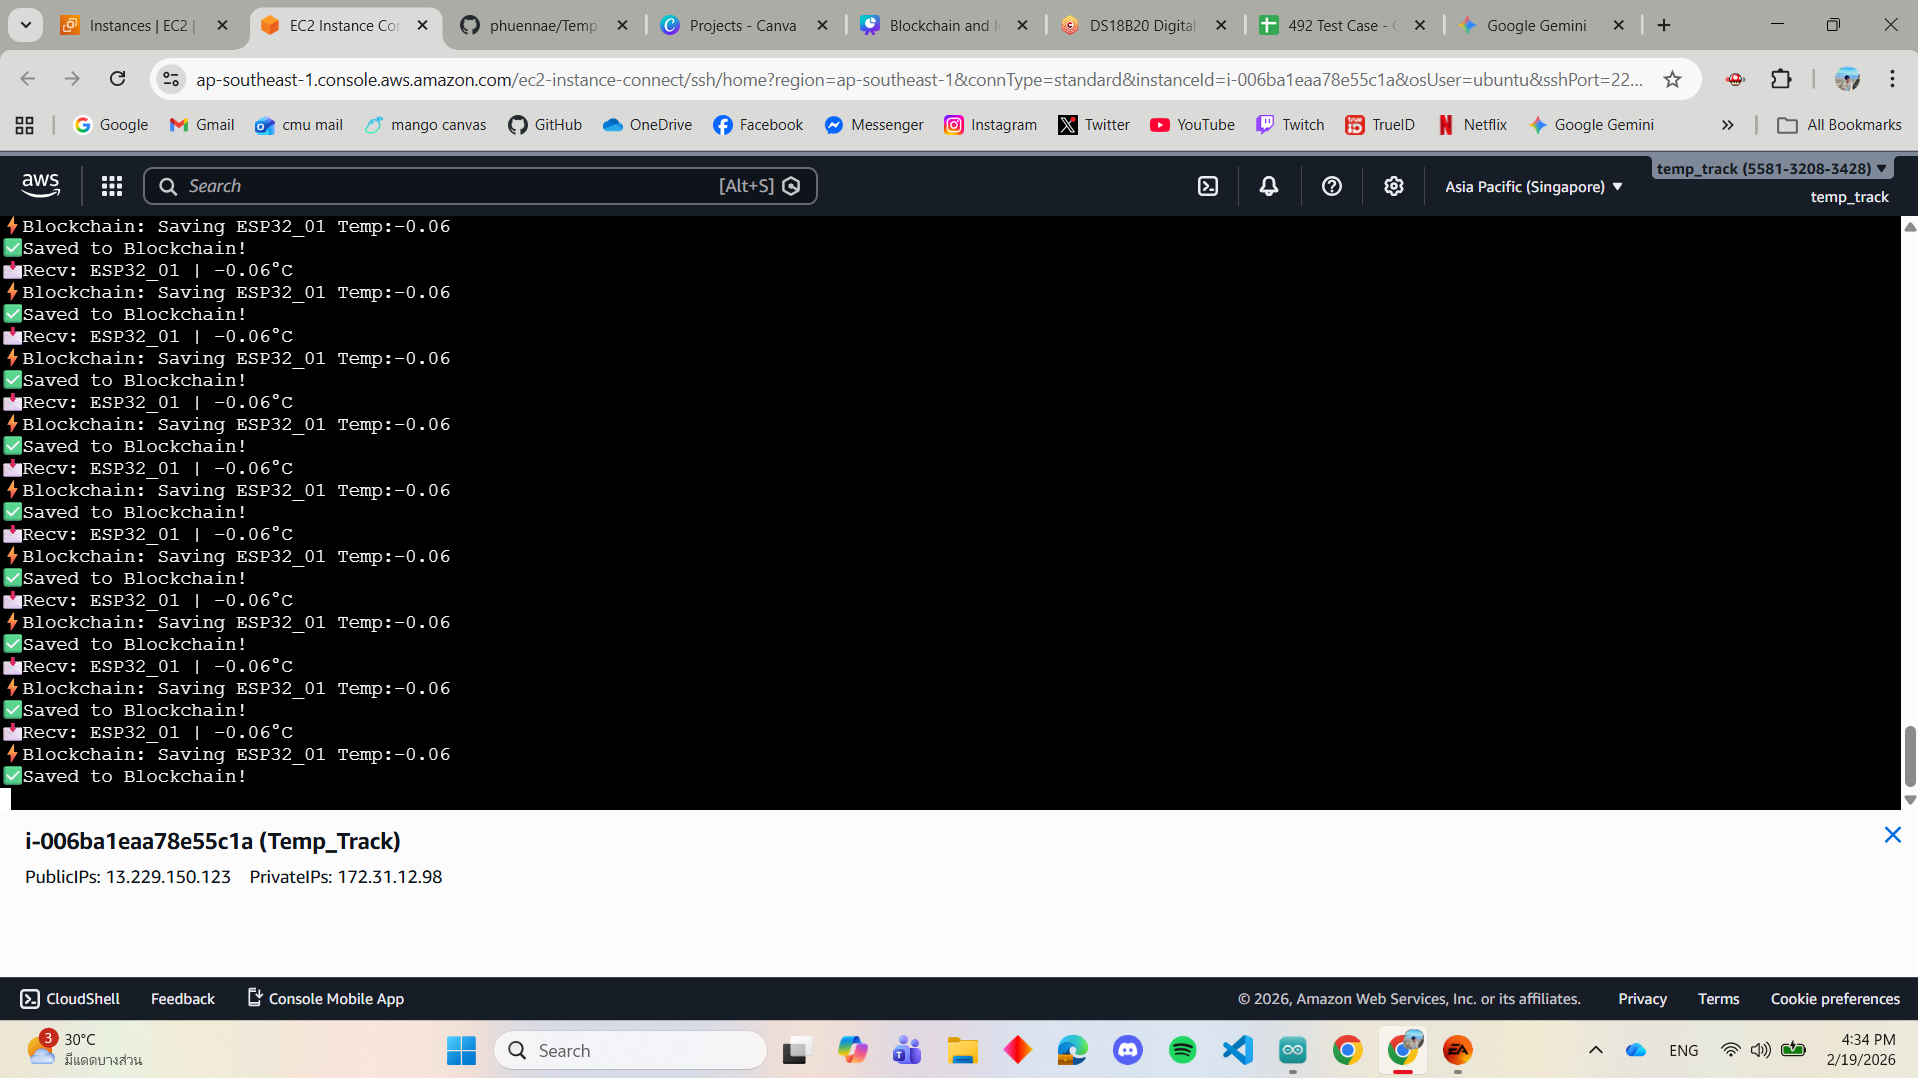
\includegraphics[width=0.85\textwidth]{AWS EC2 Server Terminal.png} 
    \caption{หน้าจอแสดงผลการทำงานขณะระบบรับข้อมูลและบันทึกลงบล็อกเชนสำเร็จ}
    \label{fig:backend_terminal}
\end{figure}


\chapter{รายละเอียดฮาร์ดแวร์และการต่อวงจร}

\section{การต่อวงจรเซ็นเซอร์อุณหภูมิและบอร์ดควบคุม}
ในส่วนนี้แสดงแผนผังการต่อสายระหว่างบอร์ดไมโครคอนโทรลเลอร์กับเซ็นเซอร์วัดอุณหภูมิ DS18B20

\begin{figure}[H]
     \centering
     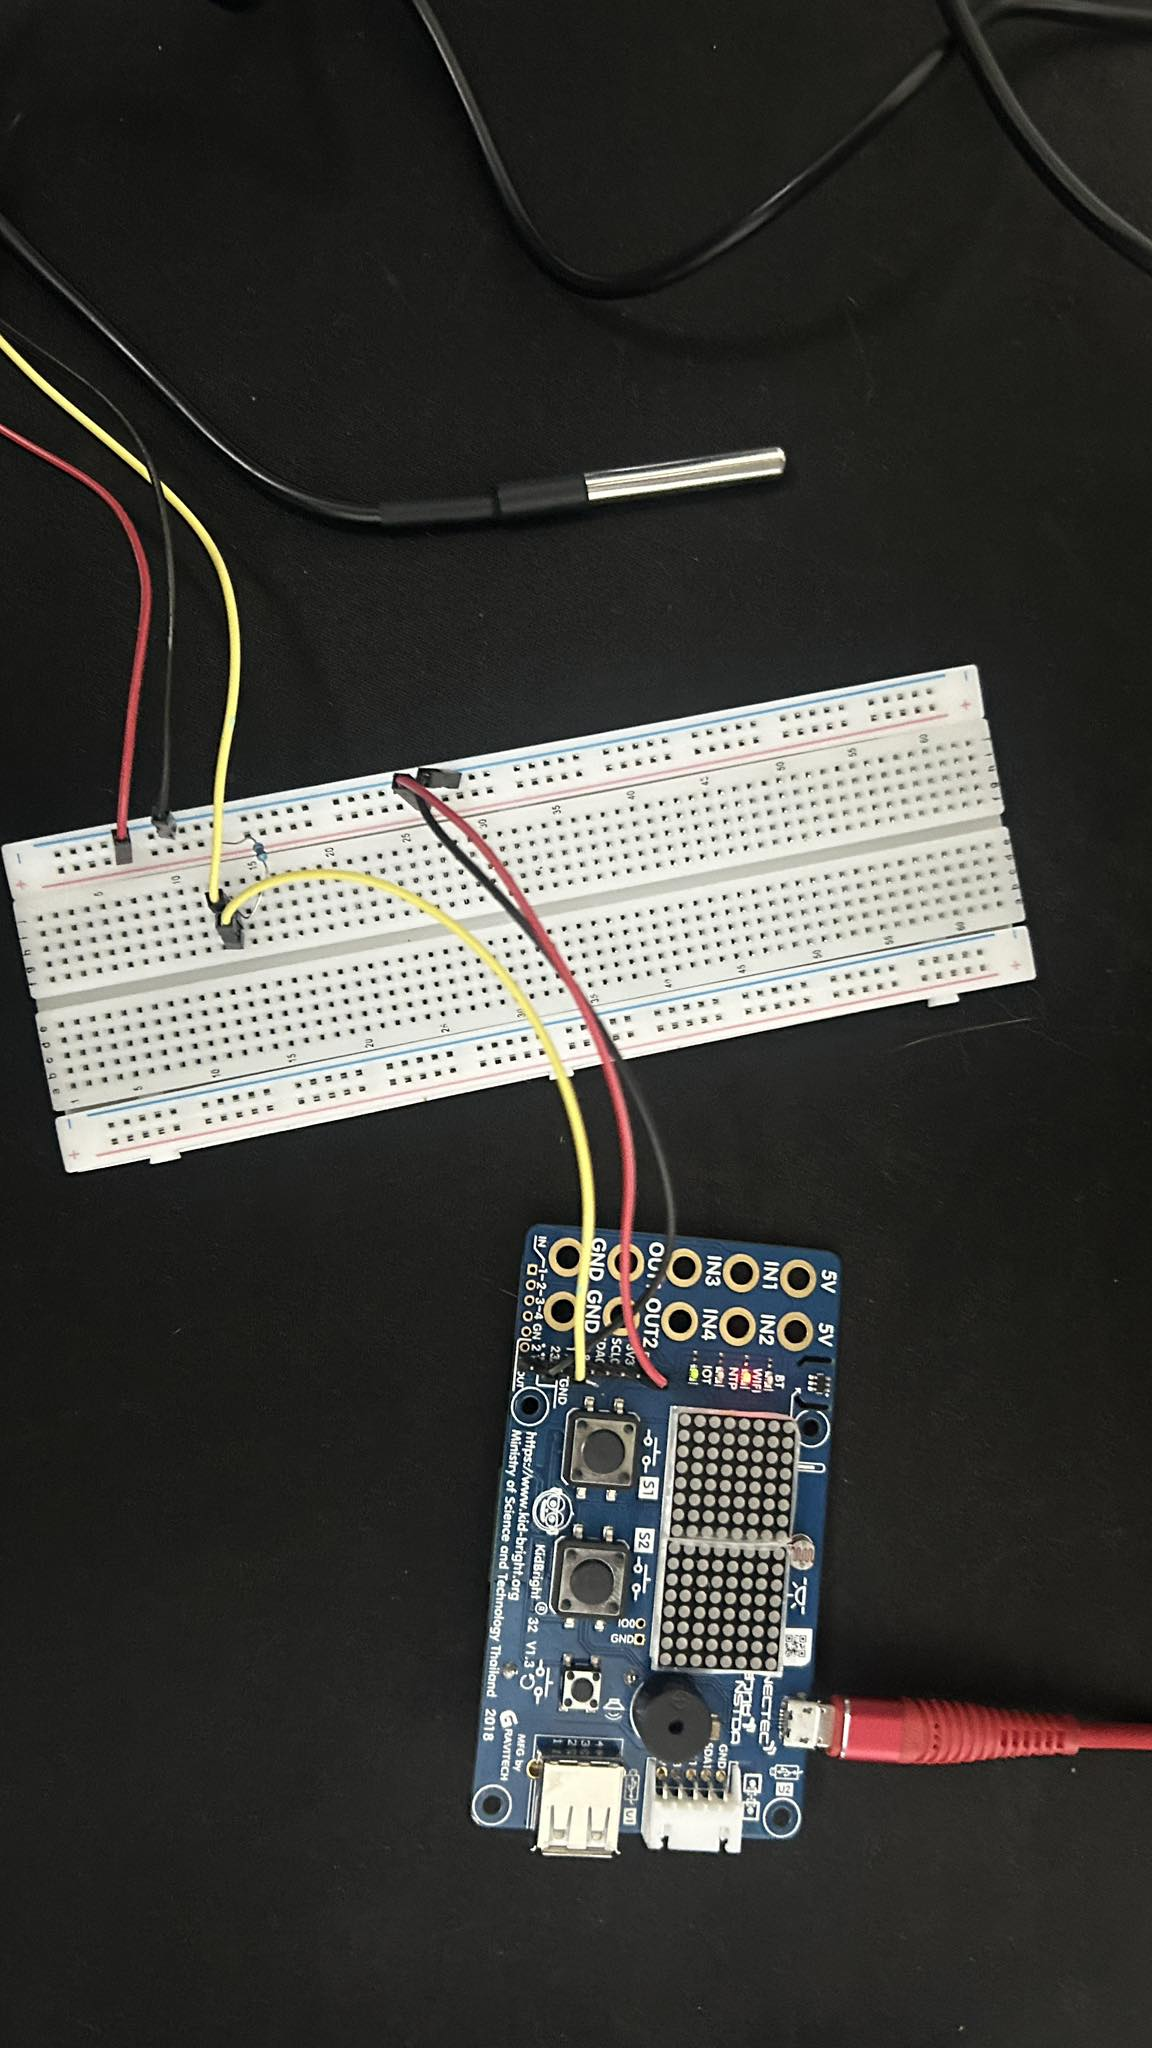
\includegraphics[angle=-90, width=0.9\textwidth]{492 wiring diagram.jpg}
     \caption{แผนผังการต่อวงจรฮาร์ดแวร์ของโปรเจกต์ TempTrack}
 \end{figure}


\chapter{โครงสร้างซอร์สโค้ด}

\section{โครงสร้างซอร์สโค้ดฝั่ง IoT}
หน้าที่ของไฟล์หลักในฝั่ง IoT มีรายละเอียดดังนี้:
\begin{itemize}
    \item[] \textbf{\texttt{DS18B20\_example.ino}} : โค้ดทดสอบการอ่านค่าอุณหภูมิเบื้องต้น
    \item[] \textbf{\texttt{Temptrack\_MQTT.ino}} : โค้ดหลักที่ใช้อ่านอุณหภูมิและส่งผ่าน MQTT
\end{itemize}

\section{ซอร์สโค้ดส่วนเชื่อมต่อข้อมูล (MQTT to Blockchain Bridge)}
ในไฟล์ \texttt{server.js} มีลอจิกสำคัญในการดักฟังข้อมูลและสั่งบันทึกลงบล็อกเชน พร้อมทั้งแสดงสถานะการทำงาน (Log) ออกทางหน้าจอ ดังนี้:

\begin{verbatim}
client.on('message', async (topic, message) => {
    const data = JSON.parse(message.toString());
    console.log(`Recv: ${data.sensor_id} | ${data.temp}`);

    try {
        await contract.submitTransaction('CreateRecord', data.temp);
        console.log('Saved to Blockchain!');
    } catch (e) {
        console.log('Error: ', e);
    }
});
\end{verbatim}

\section{โครงสร้างซอร์สโค้ดฝั่ง Web Application}
(อยู่ระหว่างการรวบรวมรายละเอียดโครงสร้างไฟล์ฝั่ง Web Application)

\newpage

%% Display glossary (optional) -- need glossary option.
% \ifglossary\glossarypage\fi

% %% Display index (optional) -- need idx option.
% \ifindex\indexpage\fi

% เปิดใช้งานประวัติผู้เขียน
\begin{biosketch}

% ==================== คนที่ 1 ====================
\begin{center}
  % เปลี่ยนชื่อไฟล์รูปในปีกกาให้ตรงกับรูปของนันท์นภัส
  
\includegraphics[width=1.5in]{meow1.jpg} 
\end{center}
\vspace{1em}

\noindent \textbf{ชื่อ-นามสกุล} นางสาวนันท์นภัส ศิริธนาโชคไพศาล \\
\textbf{รหัสนักศึกษา} 650610776 \\
\textbf{การศึกษา} ปริญญาตรี สาขาวิศวกรรมคอมพิวเตอร์ คณะวิศวกรรมศาสตร์ มหาวิทยาลัยเชียงใหม่ \\
\textbf{E-mail} nunnapats2940@gmail.com

\vspace{3em} % เว้นระยะห่างก่อนขึ้นคนต่อไป (หรือเปลี่ยนเป็น \newpage ถ้าอยากให้ขึ้นหน้าใหม่เลย)

% ==================== คนที่ 2 ====================
\begin{center}
  % เปลี่ยนชื่อไฟล์รูปในปีกกาให้ตรงกับรูปของปิ่นนารี
  
\includegraphics[width=1.5in]{meow2.jpg} 
\end{center}
\vspace{1em}

\noindent \textbf{ชื่อ-นามสกุล} นางสาวปิ่นนารี พร้อมมิตร \\
\textbf{รหัสนักศึกษา} 650610785 \\
\textbf{การศึกษา} ปริญญาตรี สาขาวิศวกรรมคอมพิวเตอร์ คณะวิศวกรรมศาสตร์ มหาวิทยาลัยเชียงใหม่ \\
\textbf{E-mail} pprommitr@gmail.com
\vspace{3em} 

% ==================== คนที่ 3 ====================
\begin{center}
  % เปลี่ยนชื่อไฟล์รูปในปีกกาให้ตรงกับรูปของผืนป่า
  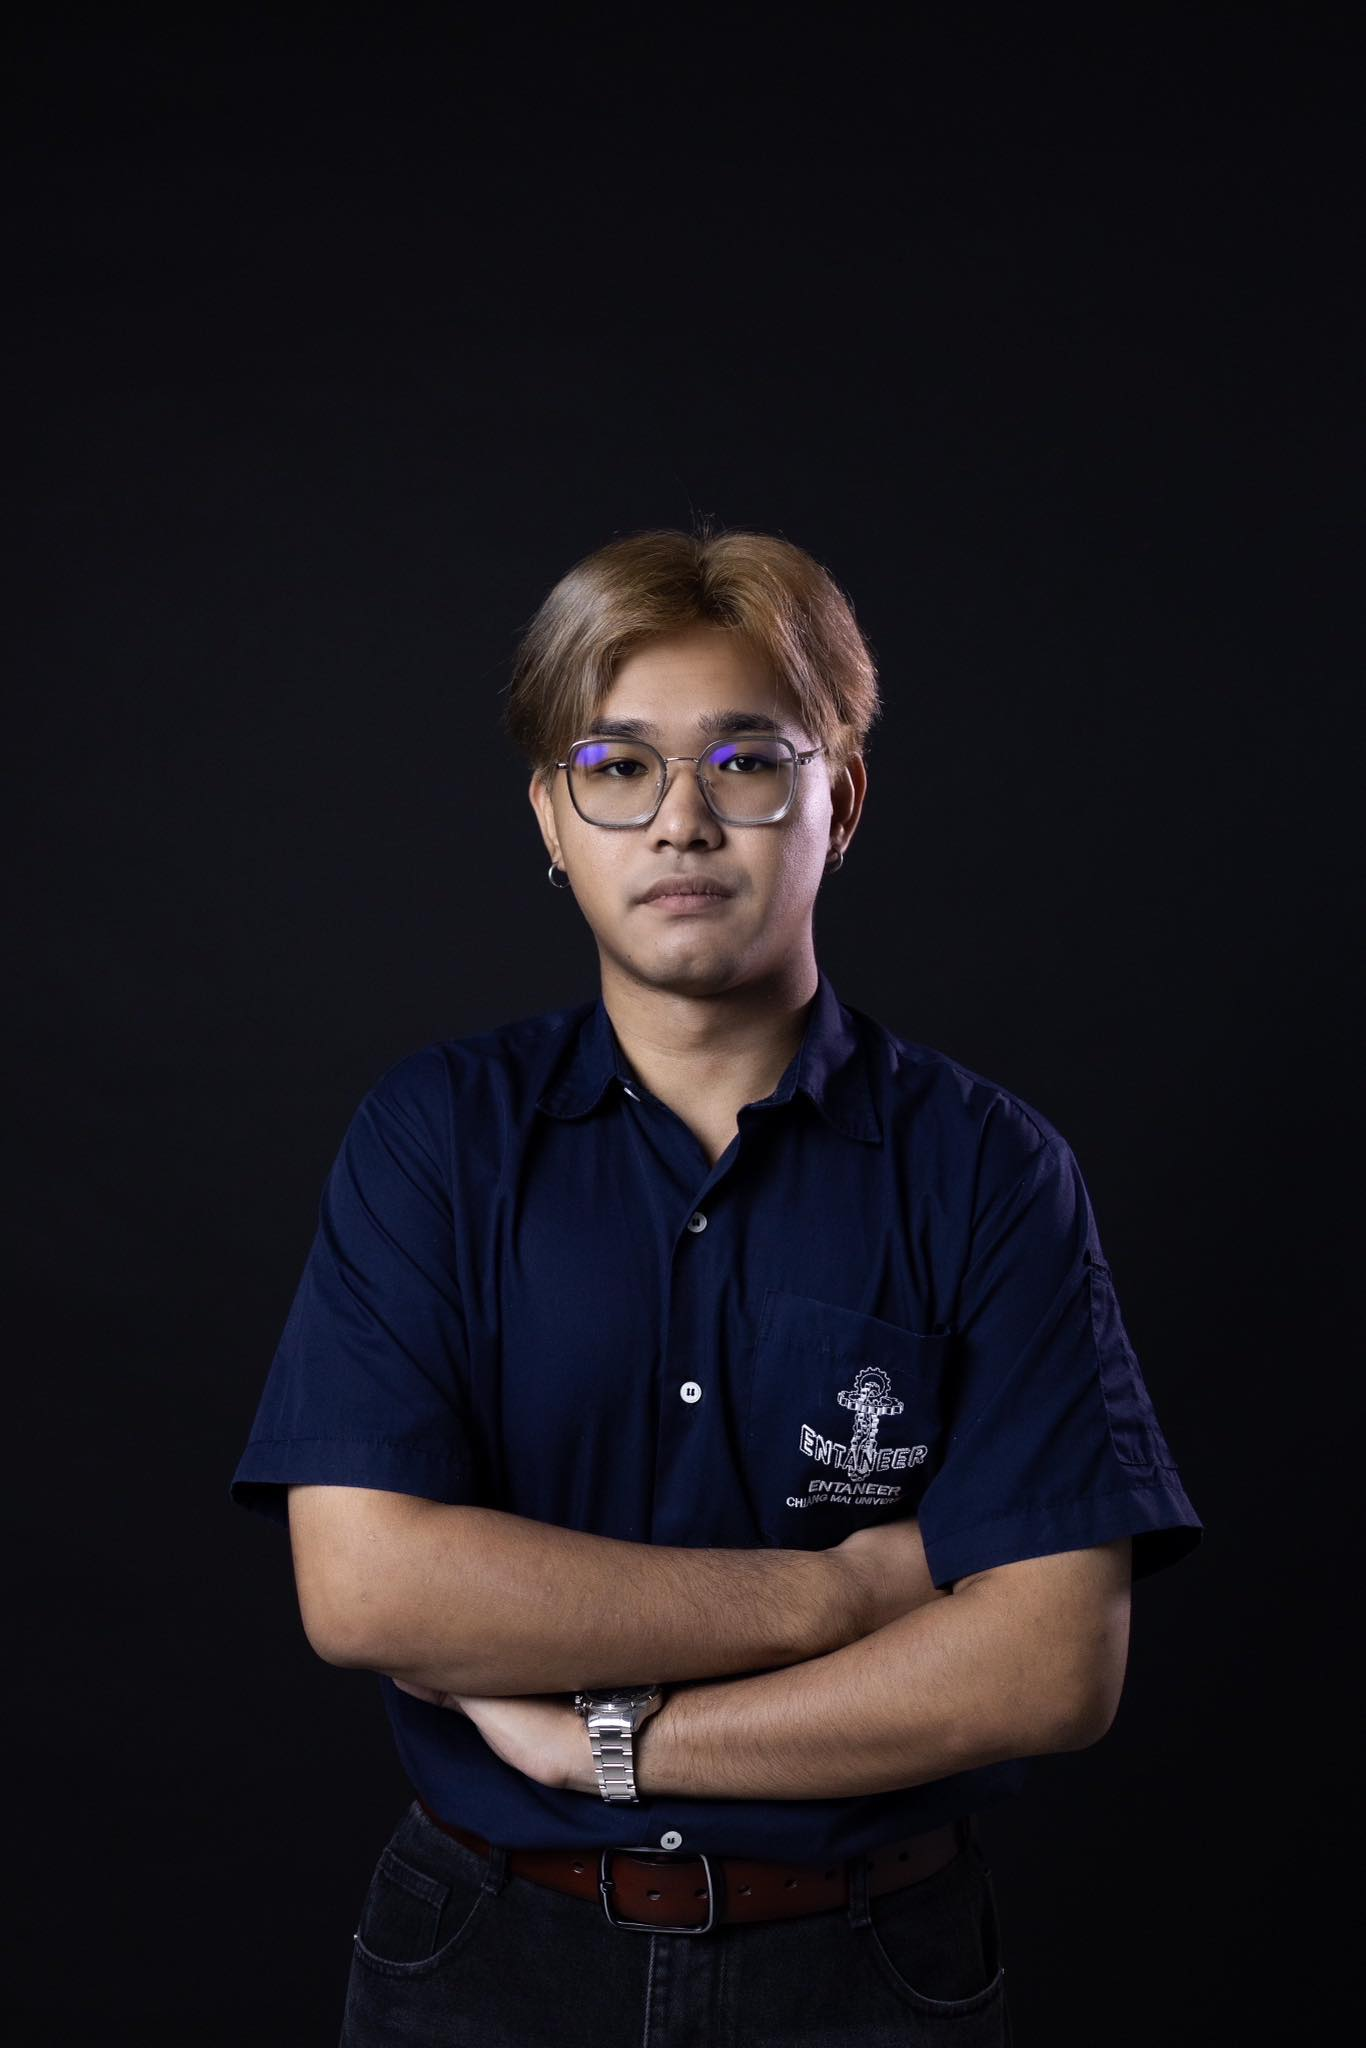
\includegraphics[width=1.5in]{phuenpa.jpg} 
\end{center}
\vspace{1em}

\noindent \textbf{ชื่อ-นามสกุล} นายผืนป่า จำปาศรี \\
\textbf{รหัสนักศึกษา} 650612090 \\
\textbf{การศึกษา} ปริญญาตรี สาขาวิศวกรรมคอมพิวเตอร์ คณะวิศวกรรมศาสตร์ มหาวิทยาลัยเชียงใหม่ \\
\textbf{E-mail} phuenpach@gmail.com
\end{biosketch}
\fi  

\end{document}